%%%%%%%%%%%%%%%%%%%%%%% file template.tex %%%%%%%%%%%%%%%%%%%%%%%%%
%
% This is a general template file for the LaTeX package SVJour3
% for Springer journals.          Springer Heidelberg 2010/09/16
%
% Copy it to a new file with a new name and use it as the basis
% for your article. Delete % signs as needed.
%
% This template includes a few options for different layouts and
% content for various journals. Please consult a previous issue of
% your journal as needed.
%
%%%%%%%%%%%%%%%%%%%%%%%%%%%%%%%%%%%%%%%%%%%%%%%%%%%%%%%%%%%%%%%%%
%
\RequirePackage{fix-cm}
%
%\documentclass{svjour3}                     % onecolumn (standard format)
%\documentclass[smallcondensed]{svjour3}     % onecolumn (ditto)
\documentclass[smallextended]{svjour3}       % onecolumn (second format)
%\documentclass[twocolumn]{svjour3}          % twocolumn
%
\smartqed  % flush right qed marks, e.g. at end of proof
%
\usepackage{graphicx}
\usepackage{amsmath,amssymb,url,times}%,subfigure}% amsthm is the one!
\usepackage{caption,subcaption,hyperref}
\usepackage{color,comment}
\usepackage{curves,pgfgantt}
\usepackage[linesnumbered,ruled,vlined]{algorithm2e} 
\usepackage{hyperref}
% \usepackage{mathptmx}      % use Times fonts if available on your TeX system
%
% insert here the call for the packages your document requires
%\usepackage{latexsym}
% etc.
%
% please place your own definitions here and don't use \def but
% \newcommand{}{}
%
% Insert the name of "your journal" with
 \journalname{Journal of Intelligent \& Robotic Systems}

\newtheorem{prop}{Proposition}
\newcommand{\norm}[1]{\ensuremath{\left\| #1 \right\|}}
\newcommand{\abs}[1]{\ensuremath{\left| #1 \right|}}
\newcommand{\bracket}[1]{\ensuremath{\left[ #1 \right]}}
\newcommand{\braces}[1]{\ensuremath{\left\{ #1 \right\}}}
\newcommand{\parenth}[1]{\ensuremath{\left( #1 \right)}}
\newcommand{\ip}[1]{\ensuremath{\langle #1 \rangle}}
\newcommand{\refeqn}[1]{(\ref{eqn:#1})}
\newcommand{\reffig}[1]{Figure \ref{fig:#1}}
\newcommand{\tr}[1]{\mbox{tr}\ensuremath{\negthickspace\bracket{#1}}}
\newcommand{\trs}[1]{\mbox{tr}\ensuremath{\!\bracket{#1}}}
\newcommand{\deriv}[2]{\ensuremath{\frac{\partial #1}{\partial #2}}}
\newcommand{\G}{\ensuremath{\mathsf{G}}}
\newcommand{\SO}{\ensuremath{\mathsf{SO(3)}}}
\newcommand{\T}{\ensuremath{\mathsf{T}}}
\renewcommand{\L}{\ensuremath{\mathsf{L}}}
\newcommand{\so}{\ensuremath{\mathfrak{so}(3)}}
\newcommand{\SE}{\ensuremath{\mathsf{SE(3)}}}
\newcommand{\se}{\ensuremath{\mathfrak{se}(3)}}
\renewcommand{\Re}{\ensuremath{\mathbb{R}}}
\newcommand{\Sph}{\ensuremath{\mathsf{S}}}
\newcommand{\aSE}[2]{\ensuremath{\begin{bmatrix}#1&#2\\0&1\end{bmatrix}}}
\newcommand{\ase}[2]{\ensuremath{\begin{bmatrix}#1&#2\\0&0\end{bmatrix}}}
\newcommand{\D}{\ensuremath{\mathbf{D}}}
\renewcommand{\d}{\ensuremath{\mathbf{d}}}
\newcommand{\pair}[1]{\ensuremath{\left\langle #1 \right\rangle}}
\newcommand{\met}[1]{\ensuremath{\langle\!\langle #1 \rangle\!\rangle}}
\newcommand{\Ad}{\ensuremath{\mathrm{Ad}}}
\newcommand{\ad}{\ensuremath{\mathrm{ad}}}
\newcommand{\g}{\ensuremath{\mathfrak{g}}}
\newcommand{\argmin}{\operatornamewithlimits{argmin}}
\newcommand{\argmax}{\operatornamewithlimits{argmax}}
\graphicspath{{../../Fig/}}
\newcommand{\WriteBlue}[1]{{\color{blue}\protect #1}}

\begin{document}

\title{Bayesian Mapping-Based Autonomous Exploration and Patrol of 3D Structured Indoor Environments with Multiple Flying Robots}
%\title{Multi-Vehicle Cooperative Exploration and Patrol of Uncertain 3D Environments}

%\titlerunning{Short form of title}        % if too long for running head

\author{Evan Kaufman \and Kuya Takami \and \\ Zhuming Ai \and Taeyoung Lee}%


% Expanded:
\institute{E. Kaufman \at
              Dept. of Mechanical and Aerospace Engineering \\
		 The George Washington University \\
		 Washington DC 20052 \\
              Tel.: 216-346-0946\\
              \email{evankaufman@gwu.edu} 
           \and
           K. Takami \at
              Dept. of Mechanical and Aerospace Engineering \\
		 The George Washington University \\
		 Washington DC 20052 \\
              Tel.: 414-212-5155\\
              \email{kuya@gwu.edu} 
           \and
           T. Lee \at
              Dept. of Mechanical and Aerospace Engineering \\
		 The George Washington University \\
		 Washington DC 20052 \\
              Tel.: 202-994-8710\\
		 Fax: 202-994-0238\\
              \email{tylee@gwu.edu}
           \and
           Z. Ai \at
              Information Management \& Decision Architectures
              \\ U.S. Naval Research Laboratory \\
              Washington, DC 20375
}

% Condensed:
\institute{E. Kaufman, K. Takami, and T. Lee \at
              Dept. of Mechanical and Aerospace Engineering \\
		 The George Washington University \\
		 Washington DC 20052 \\
              Tel.: 202-994-8710\\
              \email{\{evankaufman,kuya,tylee\}@gwu.edu} 
           \and
           Z. Ai \at
              Information Management \& Decision Architectures
              \\ U.S. Naval Research Laboratory \\
              Washington, DC 20375
}




\date{Received: date / Accepted: date}


\maketitle

\begin{abstract}
Mobile robots are frequently faced with mapping and exploring uncertain environments in surveillance, military, and convenience tasks. Often times, human teleoperation is either inconvenient or infeasible for these kinds missions. Furthermore, these tasks can be improved by cooperative multi-agent systems, where coordinating robotic efforts can be complicated and computationally-expensive. This paper presents a stochastic framework for autonomous exploration and patrol with multiple cooperating robots. The first contribution extends the authors' prior work in single-robot exact occupancy grid mapping and autonomous exploration in a 2D environment to mapping and exploring in a 3D environment. The proposed 3D occupancy grid map is computed efficiently using an inverse sensor model that accounts for the sensor uncertainty, where we propose how several measurement sources may be fused together by considering depth readings individually. This approach is scalable to larger and more complex scenarios for real-time mapping. Furthermore, this paper shows how important aspects of a 3D map representing a structured environment are projected onto a 2D occupancy grid map, where an autonomous exploration algorithm is designed to select robotic motions that maximize map information gain. The mapping and exploration algorithms are demonstrated with an experiment where a quadrotor autonomously maps and explores an initially-uncertain environment. The second contribution is a novel approach to multi-vehicle cooperative patrol of environments based on map uncertainty. We propose a cooperative autonomous exploration algorithm, which applies a bidding-based framework to coordinate robotic efforts for improving occupancy grid map information gain. Since these exploration approaches are based on probabilistic knowledge about the map, the 3D occupancy grid map is systematically degraded over time to encourage the robots to revisit regions as time passes, thereby patrolling the environment. Furthermore, using a Bayesian framework and receding horizons, the algorithm is robust to dynamic obstacles within the mapping space. The efficacy of the proposed multi-vehicle cooperative patrol is illustrated with a simulation involving three robots patrolling a large floor plan with a non-cooperative person walking around the space.
\keywords{Cooperative Patrol \and Multi-Vehicle Autonomous Exploration \and 3D Occupancy Grid Mapping}
\end{abstract}

\section{Introduction}
\label{intro}

Occupancy grid mapping is a popular choice for representing the environment surrounding robots. Accurate map generation provides important information for applications such as search-and-rescue, surveillance, and robotic cleaning. Occupancy grid maps can further assist in autonomous exploration, where robots safely explore new territories while avoiding collisions. Additionally, several robotic tasks, particularly surveillance and cleaning, require periodic visitation to various regions of the mapped environment, motivating a means for autonomous patrol.

This paper addresses three key aspects to multi-vehicle mapping and patrol of uncertain environments. First, a novel exact solution to occupancy grid mapping previously-proposed by the authors is extended to a 3D representation. Important occupancy information from this 3D map is projected onto a 2D occupancy grid map, where an autonomous exploration algorithm is designed to maximize map information gain based on a measure known as Shannon's entropy. The second key aspect addresses multiple vehicles cooperating together in mapping and exploration. A bidding-based cooperative autonomous exploration strategy is proposed to coordinate robotic efforts to maximize global map information. Finally, we propose a novel method of multi-vehicle coordinated patrol based on the multi-vehicle autonomous exploration and map degradation.

\subsection{Probabilistic Occupancy Grid Mapping and Autonomous Exploration in 3D}

Mapping is an important and well-studied topic in robotics for understanding an environment, avoiding collisions, and efficiently planning robotic motions.
A popular approach to mapping is defining a grid-based map representation, e.g.,~\cite{WolSuk05,MeyBeiBur12,TanThoWolBus14}, because these representations are computationally tractable and simple to understand.

However, these conventional grid-based mapping representations commonly approximate occupancy probabilities of the grid cells. The \emph{inverse sensor model}, which determines the map occupancy probabilities based on depth sensor measurements, is approximated with a simplified function, providing an inexact solution. As such, the prior belief of the environment and the stochastic properties of the sensor are not properly accounted. Another popular approach is based on simulated learning trials~\cite{Thr01,ThrBurFox05,SouMaiGon12} to determine an inverse sensor model. This approach is complicated and inexact due to sensitivity of simulation errors. In short, none of the existing approaches use the sensor properties to directly obtain a Bayesian solution to occupancy probability.

The approximate nature of the occupancy probability, either by a simplified function or a learned solution, motivates an exact Bayesian solution to the inverse sensor model. In this paper, we propose a computationally-efficient algorithm to obtain this solution, which serves to generate probabilities in a 3D environment following the framework of~\cite{KauLeeAiMos16,KauTakAiLee17}. This approach approach integrates stochastic properties of all sensors and the prior map estimate, following a Bayesian framework, to obtain the exact 3D occupancy probabilities~\cite{KauTakAiLee18}. As such, it provides a unified framework for sensor fusion between multiple sensors with various properties, such as sensor accuracy and fields of view. 


The 3D occupancy grid map provides key information to produce the policies that govern robotic motion, referred to as autonomous exploration. Among several approaches to determine these map-based motions in real-time, the most popular approach is known as frontier-based exploration. Using frontiers for autonomous exploration was proposed for 2D environments in~\cite{Yam97,Yam98} and extended to 3D with a visibility metric in~\cite{SawKriSri09} and~\cite{ZhuDinLinWu15,SenWan16,KleDor13} using the Octomap representation. The main idea of this approach is that robots move toward the boarder between certain and uncertain spaces to push back the boundary of known space. However, these systematic actions are not based on any consideration of the future probabilistic map uncertainty.

An alternative approach that addresses the probabilistic map properties is based on Shannon's entropy~\cite{StaGriBur05}. This metric provides a measure of uncertainty, which is used to acquire expected map information gain in~\cite{KauAiLee16,KauTakAiLee17}. Furthermore, entropy-based autonomous exploration approaches can be extended to 3D in a numerically efficient manner~\cite{KauTakAiLee18}. Due to several challenges with obtaining expected information gain of 3D measurement scans, particularly with the extended computational load, we propose a numerically efficient scheme that projects stochastic properties of the 3D probabilistic occupancy grid to 2D spaces for optimal information gain and collision avoidance. This approach is appropriate for floor plans with typically low variation along the vertical direction by exploiting just the important characteristics of 3D maps within a 2D plane. This process is designed for real-time implementation by combining 3D mapping and 2D exploration in a computationally-efficient manner.

In this paper, we present a flight experiment for the proposed single-vehicle exploration scheme. Multiple tasks, such as flight control, sensor data acquisition, mapping, exploration, and communications are executed simultaneously in a ROS environment using Python/C++. These tasks are verified with a quadrotor unmanned aerial vehicle holding an ASUS Xtion infrared depth sensor and Hokuyo laser scanner operated by the NVidia Jetson computing module. 


\subsection{Multi-Vehicle Cooperative Autonomous Exploration}

Exploration with multiple robots can be beneficial in large or complicated environments to complete the task quickly and efficiently. Here, we propose a bidding-based autonomous exploration scheme to maximize global map information. The main idea is a central executive predicts how robotic actions are expected to improve map information gain cooperatively in a probabilistic fashion. A series of auctions determines where robots should travel. During each auction, robots submit bids based on how their sensors are expected to improve the quality of the occupancy grid map. Between auctions, bids are modified to reflect the impact of other robot members on the map. Because this approach is directly based on cooperative improvement of map information, considering coverage overlap among the robots, such as the work in~\cite{SimApfBurFoxMooThrYou00}, becomes unnecessary. This multi-vehicle exploration optimization is further augmented with travel time considerations and collision avoidance among robots. In short, the proposed multi-vehicle exploration scheme employs a bidding-based framework that maximizes map information while considering multiple vehicles cooperating together, and cell degradation promotes repeatedly visiting regions for patrol.

Furthermore, this bidding-based exploration approach is integrated with a receding horizon framework to optimize map information and collision-avoidance in a dynamic environment. The receding horizon framework serves to update the exploration strategy with a possibly-changing occupancy grid map, which directly impacts the viability of pose candidates. Additionally, a receding horizon provides an optimal feedback policy that can handle dynamic obstacles, improving collision-avoidance with cooperative robots and other moving obstacles, which is essential for patrolling dynamic environments.


\subsection{Multi-Vehicle Cooperative Autonomous Patrol}

Robotic surveillance and cleaning are examples of tasks that require periodic observations of the same regions. Several patrolling approaches have been proposed in recent years to address this need. A popular approach is decomposing the reachable space into Voronoi diagrams~\cite{KolCar08,PorRoc10,PipChrWei13}. In~\cite{KolCar08}, edges between nodes of the Voronoi graph are heavily sensed to track intruders. In~\cite{PorRoc10}, regions of the Voronoi diagram are assigned to different robots, and issues with robots having underperforming surveillance capabilities are addressed in~\cite{PipChrWei13}. These approaches assume the map is well-known in advance, and require a Voronoi graph be generated from the map.

Other patrol approaches create new metrics about the environment. Cell periodicity is estimated in~\cite{KraFenCieDonDuc14,KraFenHanDuc16} by predicting and observing the long-term dynamics of objects at the same locations on an occupancy grid. This work is extended to exploring and navigating a human-populated environment for long-term autonomy. A bio-inspired approach is proposed in~\cite{ZhaXia11}, where robots cooperate by dropping digital pheromones based on the importance of events, where the pheromones weaken over time to prioritize future tasks. Another approach is formulating patrol as an optimization problem with respect to robot idleness in~\cite{YanZha16}.

In this paper, the proposed approach to coordinated patrol is based on cooperative multi-vehicle autonomous exploration and map degradation, which is different from prior work in two key ways. First, the patrol is based on map uncertainty, where the environment can be initially-uncertain. Second, the proposed approach is independent of external variables or structures such as Voronoi diagrams, cell periodicity estimates, digital pheromones, or idleness estimates. Instead, the proposed patrol approach is based on predicting future occupancy grid cell uncertainties. All grid cells are subjected to a continuous-time Markov degradation process. Highly certain cells subject to this Bayesian process slowly increase in uncertainty over time. Then, the multi-vehicle exploration scheme assigns cooperating robots to revisit these cells. Thus, degradation promotes periodic observations of different regions of the map.

We present a numerical simulation of three quadrotors mapping and patrolling a floor plan of a building, which is initially uncertain. The robots must safely patrol this space while a human walks independently around the environment.

In short, the contributions of this paper are as follows. First, we propose a computation technique to extend 2D mapping and autonomous exploration to a 3D environment in real-time. Then, we propose a bidding-based cooperative exploration with multiple vehicles. The exploration is developed in a receding horizon framework for dynamic environments. Finally, we develop a stochastic framework for patrol. These are demonstrated with an experiment and a simulation.


\section{Problem Formulation}
\label{sec:ProbDef}

This sections summarizes the key equations providing the exact solutions to occupancy grid mapping and expected entropy change proposed in~\cite{KauLeeAiMos16,KauTakAiLee17,KauTakAiLee18,KauAiLee16}.

\subsection{Probabilistic Occupancy Grid Mapping}
\label{subsec:POGM}
An occupancy grid map $m$ is composed of $n_m$ grid cells, where each grid cell is a cube with fixed edge length $\alpha$. Occupancy grid cells are considered static binary random variables, i.e., the $i$-th grid cell $\mathbf{m}_i=1$ if occupied or $\mathbf{m}_i=0$ if free (unoccupied). For convenience, we define its complement as $\bar{\mathbf{m}}_i=1-\mathbf{m}_i$ such that $P(\bar{\mathbf{m}}_i)=1-P(\mathbf{m}_i)$. Since we assume grid cell occupancies are mutually independent, $2^{n_m}$ map combinations are possible.

The occupancy grid map cell probabilities are repeatedly updated by a range sensor. Through the $t$-th time step, we assume the history of poses $X_{1:t}$ and measurement scans $Z_{1:t}$ are given. The $t$-th pose $X_t=\braces{x_t,R_t}$ consists of position $x_t\in\Re^3$ and attitude $R_t\in\SO=\braces{R\in\Re^{3\times3}|R^\T R=I,\det{R}=1}$. However, measurements are subject to random noise; let individual measurement ray $z\in Z_t$ be characterized by the \emph{forward sensor model}, which is a probability density $p(z|X_t,m)$, known either from the sensor manufacturer or obtained empirically. The goal of probabilistic occupancy grid mapping is using the stochastic properties of the forward sensor model to obtain the \emph{inverse sensor model}, $P(m|z,X_{1:t},Z_{1:t-1})$.

\sloppy
The inverse sensor model problem was solved in~\cite{KauLeeAiMos16,KauTakAiLee17} to provide a real-time solution that uses the forward sensor model directly with map invariance. The process is fairly straightforward: define a reduced map $r\subset m$ of $n_r$ grid cells along $z$, indexed by increasing distance. Let $\mathbf{r}_{k+}$ correspond to the $k$-th cell being the closest occupied space. Then, the inverse sensor model is
\begin{align}
\label{eqn:RayISMAnswer}
P(\mathbf{r}_{k}|z,X_{1:t},Z_{1:t-1})&=\eta\tilde P(\mathbf{r}_{k}|z,X_{1:t},Z_{1:t-1}),
\end{align}
where $\eta$ is the normalizer,
\begin{align}
\label{eqn:allEta}
\eta
&=
\bigg[\sum_{i=1}^{n_{r}+1}\bigg\{\prod_{j=0}^{i-1}\bar{\mathbf{P}}_j^-\bigg\} p(z|\mathbf{r}_{i+},X_t)\mathbf{P}_i^-\bigg]^{-1},
\end{align}
such that the summation of any cell probability and its complement is $1$. The unnormalized probability of the inverse sensor model is defined as
\begin{align}
\label{eqn:Unnormalized}
\tilde P(\mathbf{r}&_{k}|z,X_{1:t},Z_{1:t-1})\nonumber\\
&=\mathbf{P}_k^-
\bigg[\sum_{i=1}^{k-1}\bigg\{\prod_{j=0}^{i-1}\bar{\mathbf{P}}_j^-\bigg\}p(z|\mathbf{r}_{i+},X_t)\mathbf{P}_k^-\bigg]+ \bigg\{\prod_{j=0}^{k-1}\bar{\mathbf{P}}_j^-\bigg\}p(z|\mathbf{r}_{k+},X_t)\mathbf{P}_k^-,
\end{align}
where probability $\mathbf{P}_k^-=P(\mathbf{r}_{k}|X_{1:t-1},Z_{1:t-1})$ and its complement $\bar{\mathbf{P}}_k^-=1-\mathbf{P}_k^-$ are known a priori, we select $P(\bar{\mathbf{r}}_{0}|X_{1:t-1},Z_{1:t-1})=P(\mathbf{r}_{n_r+1}|X_{1:t-1},Z_{1:t-1})=1$ for convenience, and the forward sensor model maximum reading case is $p(z|\mathbf{r}_{(n_r+1)+},X_t)$. The proofs are given in~\cite{KauLeeAiMos16} for \refeqn{RayISMAnswer}--\refeqn{Unnormalized}. Since these equations use several repeated terms, \refeqn{RayISMAnswer} exhibits linear complexity with respect to the number of cells along a measurement ray, amortized to $\mathcal{O}(1)$ for each cell, so the exact inverse sensor model can be applied in real-time.

\subsection{Predictive Entropy-Based Autonomous Exploration}

Here we introduce Shannon's entropy as a measure of probabilistic map uncertainty~\cite{StaGriBur05}, which provides key information for optimal motion planning. Shannon's entropy is defined as
\begin{align}
\label{eqn:ShannonsEntropyCell}
H(P(\mathbf{m}_i))&=-P(\mathbf{m}_i)\log{P(\mathbf{m}_i})-P(\bar{\mathbf{m}}_i)\log{P(\bar{\mathbf{m}}_i}),
\\
\label{eqn:ShannonsEntropyMap}
H(P(m))&=\sum_{i=1}^{n_m}H(P(\mathbf{m}_i)),
\end{align}
for a single grid cell and the entire map, respectively.
Thus, $P(\mathbf{m}_i)=0.5$ maximizes \refeqn{ShannonsEntropyCell}, corresponding to the largest uncertainty; similarly, \refeqn{ShannonsEntropyCell} is minimized as $P(\mathbf{m}_i)$ approaches $0$ or $1$, corresponding to the smallest uncertainty. 

Suppose a future pose candidate and its associated future measurement scan is $X_c=\braces{x_c,R_c}$ and $Z_c$, respectively, where $c\in\mathcal C$ such that $\mathcal C=\braces{1,2,...,n_c}$ accounts for all $n_c$ candidates under consideration for the next robot pose. The current pose of the robot is \emph{not} $X_c$ in general, so changes to the probabilistic map from $X_c$ can only be predicted. 
This is achieved by considering the expected entropy change of individual measurement rays~\cite{KauAiLee16,KauTakAiLee17}. Removing $X_{1:t}$ and $Z_{1:t}$ for simplicity, the expected entropy for candidate ray $z_c$ is
\begin{align}
\label{eqn:DiscExpEntropyRay}
&\text{E}[H(P(m|x_c,z_{c}))]=\sum_{k=1}^{n_{r}+1}\bigg\{H(P(m|x_c,z_{c,k}))P(z_{c,k}|x_c)\bigg\},
\end{align}
where $z_{c,k}$is distance along measurement ray $z_{c}$ from position $x_c$ to the $k$-th grid cell. The first term in \refeqn{DiscExpEntropyRay}, namely $H(P(m|x_c,z_{c,k}))$, is found with the inverse sensor model \refeqn{RayISMAnswer}--\refeqn{Unnormalized} and grid cell entropy \refeqn{ShannonsEntropyCell}--\refeqn{ShannonsEntropyMap}.
The second term is derived from \refeqn{allEta} with
\begin{align}
\label{eqn:ProbMeas}
P(z_{c,k}|x_c)&=\frac{p(z_{c,k}|x_c)}{\sum_{i=1}^{n_{r}+1}p(z_{c,i}|x_c)}=\frac{\eta_{c,k}^{-1}}{\sum_{i=1}^{n_{r}+1}\eta_{c,i}^{-1}},
\end{align}
where $\eta_{c,k}$ refers to the normalizer based on the measurement $z_{c,k}$.
The expected negative entropy change for candidate pose $X_c$ is equivalently the expected information gain,
\begin{align}
\label{eqn:expectedInfoGainRay}
\mathcal I(X_c)&=H(P(m|X_{1:t},Z_{1:t}))-\text{E}\left[H(P(m|X_c,Z_c))\right].
\end{align}
Then, we repeat \refeqn{DiscExpEntropyRay} for several sample measurement rays composing scan $Z_c$~\cite{KauAiLee16}.



\section{Mapping and Exploring in 3D}

In this section, we present computational techniques to implement the probabilistic mapping and exploration schemes discussed in the prior section to a 3D environment in real-time with explicit consideration of the computation time.

\subsection{Mapping in 3D Space}

Grid cells along a measurement ray are updated using the inverse sensor model. Since a measurement ray is assumed to follow a straight line, the inverse sensor model is evaluated only along that vector. Prior research~\cite{KauLeeAiMos16,KauTakAiLee17} is based on 2D distances from the robot to grid cells, which are obtained geometrically through ray casting. This approach is easily extended to 3D space, where the inverse sensor model is applied identically after ray casting. Each measurement ray is considered individually, which simplifies measurement fusion from any number of sensors with differing stochastic properties. Furthermore, multiple sensor scans may update the map in parallel threads, thereby increasing the number of measurements to update the 3D map. In short, extending the exact inverse sensor model from 2D to 3D with multiple sensors involves straightforward geometry for ray casting and processing the sensor readings in parallel.

A robot might be equipped with multiple sensors for several reasons, e.g., different depth accuracy or fields-of-view. For example, consider a robot carying a 2D LIDAR providing highly accurate measurements over a horizontal plane. This sensor might rapidly update the grid cells at the robot height, but neglect spaces above or below the robot. The robot can compensate for these limitations with an IR depth sensor providing measurements with nonzero components in the vertical direction, even if the IR depth sensor accuracy is lower than the LIDAR accuracy. Measurements from both sensors may update the same probabilistic map because each sensor model is explicitly considered in the cell probability calculations. In short, the proposed 3D mapping approach can fuse the impact of measurements on the probabilistic map from different sources because the stochastic properties of measurements are considered according to a Bayesian framework explicitly.


However, several careful considerations are required for 3D implementation. First, increasing the map dimensions from 2D to 3D requires memory reserves to multiply by a factor of the number of cells in the added dimension. Second, rays spanning 3D space tend to intersect more grid cells than rays spanning 2D space, which increases the number of grid cells updated per ray. Computation time for the inverse sensor model is linear with respect to the number of cells considered, so careful considerations on sensor limits and number of rays updated per scan are important.
It is common that computers onboard flying robots lack the processing capabilities to update massive 3D maps quickly due to these limitations. Therefore, a simple solution is to stream the sensor data from an onboard computer to a more powerful computer that runs the mapping.

Additionally, mobile robots, particularly aerial vehicles, frequently make fast movements, which may cause time synchronization issues. The most problematic cases correspond to pose estimates and depth sensor readings not synchronizing. For example, the time stamps from the most recent pose estimate and measurement scan may be significantly different while the robot is rapidly rotating. Combining this pose and scan together violates the assumption that the robot pose is well-known for every measurement scan, i.e., $X_t$ and $Z_t$ are given. Therefore, pose estimates and sensor readings must be paired according to their time stamps. A useful tool to accomplish this requirement is the Message Filters package with the Robot Operating System (ROS), where time stamps are synchronized using recently received data of poses and measurement scans.

\subsection{Autonomous Exploration in 3D Space}

We propose an autonomous exploration strategy that selects motions that move the robot to poses that are expected to maximize information gain. The probabilistic map is used for acquiring entropy as a measure of uncertainty, and for collision avoidance. For these processes, careful consideration must be placed on computation. In particular, the computational complexity for expected entropy of a single measurement ray intersecting $n_r$ cells is $\mathcal O(n_r^2)$~\cite{KauAiLee16}. To address this issue, we propose projecting the 3D map onto a 2D occupancy grid map, which is located at the desired height of exploration. This approach corresponds to vertically-uniform environments such as rooms and hallways without complex geometries. Projecting the occupancy grid map simplifies the exploration through 3D space, and decreases $n_r$, thereby increasing the algorithm speed.


Next we describe how the 2D map projection is defined such that important information about collision and entropy is extracted from the 3D map. Let a 2D projected map be denoted $m_\text{2D}$. The two horizontal dimensions, namely $x$ and $y$, have edge length $\alpha_{xy}=k_{xy}\alpha$, where $k_{x,y}\geq1$ is an integer representing the relative edge length between the 3D map $m$ and the projected map $m_\text{2D}$. The value of $k_{x,y}$ is selected such that the area of each cell in $m_\text{2D}$ is at minimum the footprint size of the robot for simplified collision analysis. The number of cells in the vertical $z$-direction, namely $k_z\geq1$, is selected such that $k_z\alpha$ is at minimum the robot size in the vertical direction, and at maximum $k_z\alpha$ is height of the environment excluding floors and ceilings. 

Here, we show how multiple the 3D cells from map $m$ are used to find the probability of a single cell in $m_\text{2D}$. 
Let the $k$-th cell of the projected map be denoted $\mathbf{m}_{\text{2D},k}$. Let the set $a_k\subset m$ correspond to 3D cells falling within the dimensions $k_{x,y}\times k_{x,y}\times k_z$ centered at the location of $\mathbf{m}_{\text{2D},k}$. Considering that the cells begin with uniform probability $P_\text{init}$ where $0<P_\text{init}<1$, define a threshold $P_\text{thresh}$ such that $P_\text{init}<P_\text{thresh}<1$. Then, the probability of $\mathbf{m}_{\text{2D},k}$ is
\begin{align}
\label{eqn:Proj2DMapComb}
P(\mathbf{m}_{\text{2D},k})= 
\begin{cases}
    \max_{i\in a_k}{P(\mathbf{m}_i)},			&\text{if} \ \max_{i\in a_k}{P(\mathbf{m}_i)}\geq P_\text{thresh}\\
    \min_{i\in a_k}{P(\mathbf{m}_i)},              & \text{otherwise}
\end{cases}.
\end{align}
For example, if the $i$-th cell belonging to $a_k$ is considered occupied, i.e., $P(\mathbf{m}_i)>P_\text{thresh}$, then the projected 2D cell takes on the maximum probability of cells in $a_k$, and therefore is considered occupied. This conservative choice is beneficial for collision-avoidance. Alternatively, if all cell probabilities in $a_k$ fall below $P_\text{thresh}$, and the $i$-th cell probability is $P(\mathbf{m}_i)\approx0$ (typically from measurement rays passing through), then the projected cell takes on the minimum probability of cells in $a_k$, and therefore is considered free.

There are several advantages to this approach. First, the $k$-th cell probability $P(\mathbf{m}_{\text{2D},k})$ remains at $P_\text{init}$ unless the cell is measured at least once. This corresponds to a large expected information gain \refeqn{expectedInfoGainRay} for capturing this unmeasured space. Second, the collision risk is simply calculated, and can be easily modified by changing $P_\text{thresh}$. Additionally, the case when $P(\mathbf{m}_{\text{2D},k})<P_\text{thresh}$ typically implies that this cell is free, thereby increasing the impact cells further away on exploration. Furthermore, this projected map is much simpler to analyze for exploration.


\section{Multi-Vehicle Bidding-Based Autonomous Exploration}
\label{sec:BiddingExploration}

When exploring uncertain environments, robots can generate large maps much faster if they coordinate their efforts. However, the problem of determining a multi-vehicle exploration strategy is complicated and computationally expensive, but must be performed in real-time.

In this section, we formulate a cooperative and autonomous exploration scheme based on sequential auctions for maximizing map information gain. The first auction is based on the expected information gain presented in the prior section, scaled by travel distance. Once the winner of the first auction is determined, the map for bidding is updated based on the expected measurements of the first robot. The second auction for the remaining robots is determined by the information gain from the revised map that is further scaled by the travel distance and a penalty for collision-avoidance. This process is repeated until all robots are assigned tasks. 


\subsection{Objective Function for the First Auction}

Here, we describe how robots participate in the first auction for maximizing map information gain while accounting for travel time. The information gain \refeqn{expectedInfoGainRay} is computed for each candidate pose. Expected information gains may vary among the robots only if they have different sensor configurations. All expected information gains must be computed prior to the first auction.

Next, we describe how travel time is integrated into exploration. Considering that distances from current robot poses to candidate poses may differ greatly, accounting for these varying travel times properly is essential for exploration time efficiency. Travel distances are computed using Dijkstra's search to provide collision-free waypoints for each robot. There are two steps: first, generate a cost map from the robot location to each location on the 2D projected map. This provides the collision-free distances to all reachable locations on the map. Second, the waypoints from a candidate pose to the current robot pose are easily obtained along the cost map using steepest descent. 

Here, we define a bump function to account for varying travel distances from Dijkstra's search. Let the distance along the collision-free path from the $k$-th robot pose, namely $X_k$, to the $c$-th candidate pose, namely $X_c$, be denoted $d(X_k,X_c,m_\text{2D})\geq0$, which is taken from the cost map belonging to $X_k$. A continuous bump function is defined to account for traveling costs, and is composed of two parts.  

The first part of the bump function corresponds to short trajectories. Consider $d_\text{opt}$, the time-optimal distance that a robot may travel at full speed during the time between exploration updates. Here, we consider the case when $d(X_k,X_c,m_\text{2D})\leq d_\text{opt}$, i.e., the robot can completely traverse this distance during the allotted travel time. If $d(X_k,X_c,m_\text{2D})\ll d_\text{opt}$, then the robot is not moving at its full potential. This can be wasteful, because the robot tends to capture larger regions while moving. Therefore, it is desirable for $d(X_k,X_c,m_\text{2D})\rightarrow d_\text{opt}$, which corresponds to maximizing map coverage without time cost. The first part of the bump function is sinusoidal and is optimized at $d_\text{opt}$ to maximize robotic movement as
\begin{align}
\label{eqn:BumpFunIncreasing}
\mathcal B_1(d)=\frac12 f_\text{max}\left(1-\cos{\frac{d\pi}{d_\text{opt}}}\right),
\end{align}
where $f_\text{max}>0$ is the maximum value when $d(X_k,X_c,m_\text{2D})=d_\text{opt}$.

The second part of the bump function is defined over the domain where \\$d(X_k,X_c,m_\text{2D})>d_\text{opt}$ to minimize time required for $X_k$ to arrive at $X_c$, putting a penalty on traversing across the environment. This choice is beneficial to generating accurate local maps before exploring new regions. The second half is defined to be nonzero everywhere and is strictly decreasing as 
\begin{align}
\label{eqn:BumpFunDecreasing}
\mathcal B_2(d)=(f_\text{max}-f_\text{far})\exp\braces{-\beta(d_\text{opt}-d)^2}+f_\text{far},
\end{align}
where $f_\text{max}>f_\text{far}>0$ guarantees $\mathcal B_2>0$ such that $\mathcal B_2\rightarrow f_\text{far}$ as $d(X_k,X_c,m_\text{2D})\rightarrow\infty$ and $\beta>0$ assigns the rate of functional decrease relative to $f_\text{max}$ and $f_\text{far}$. Then, the complete bump function is defined as
\begin{align}
\label{eqn:BumpFun}
\mathcal B(d)=
\begin{cases}
    \mathcal B_1(d),		& \text{if }d\leq d_\text{opt},\\
    \mathcal B_2(d),         & \text{otherwise},
\end{cases}
\end{align}
which is illustrated in Fig. \ref{fig:nonzeroBumpFun}. % In short, the bump function prioritizes short movements to capture the local environment over long traversals for exploration time efficiency.

	\begin{figure}
		\centerline{
			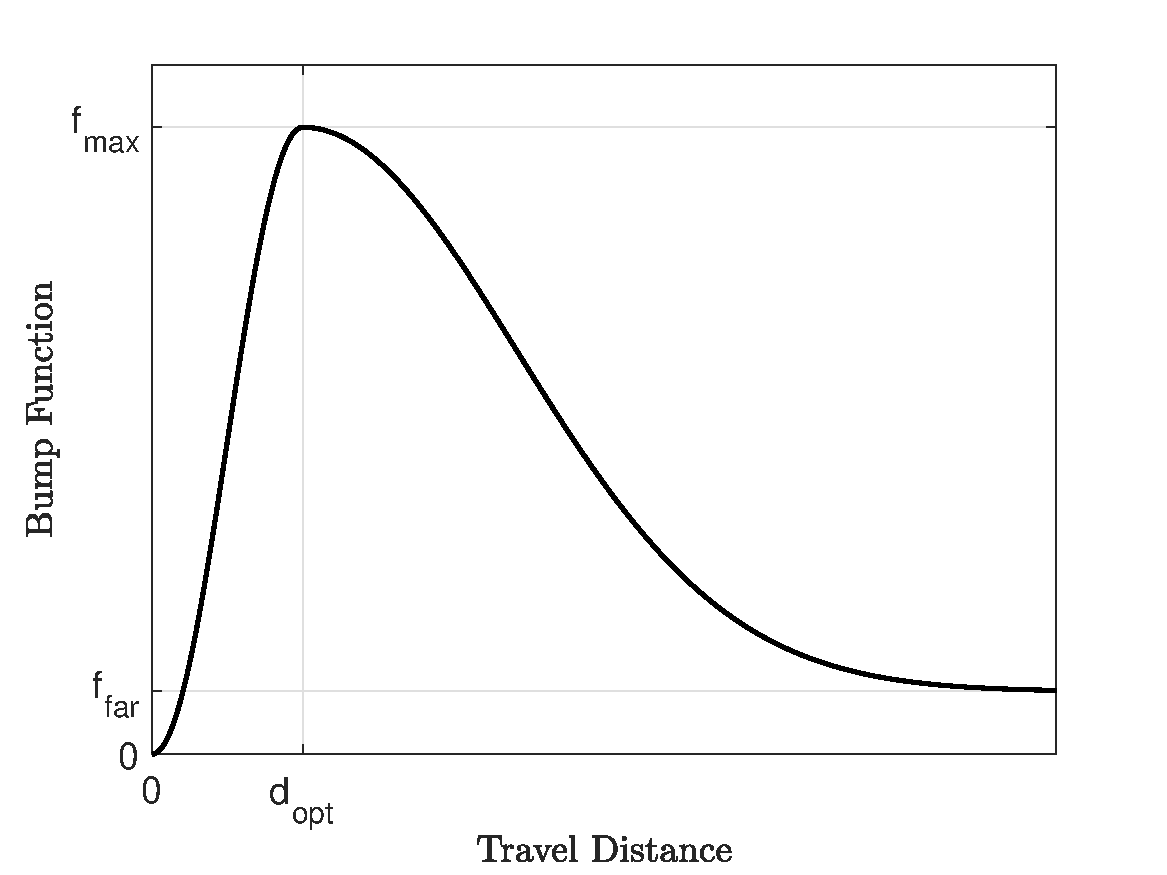
\includegraphics[width=0.9\columnwidth]{NonZeroBump.pdf}
		}
		\caption{The bump function is designed to promote travel distances close to $d_\text{opt}$ by multiplying this function by the expected information gain objective. Travel distances less than $d_\text{opt}$ are below the robot capabilities. Travel distances beyond $d_\text{opt}$ are beyond what the robot can reach within the minimum exploration computation time.}
		\label{fig:nonzeroBumpFun}
	\end{figure}
	
Then, using the information gain from \refeqn{expectedInfoGainRay} and considering the impact from travel distance from \refeqn{BumpFun}, the objective function for a single agent with respect to $X_{c}$ is
\begin{align}
\label{eqn:CandidateBidSingle}
\text{Obj}_\text{single}(X_k,X_c,m_\text{2D})&=\mathcal B(d(X_k,X_c,m_\text{2D}))\mathcal I(X_{c},m_\text{2D}).
%X_{k,c}^*&=\argmax_{X_c}{\ \mathcal B_{k,c}\mathcal I(X_c)},
\end{align}
Then, the optimal pose selection for the $k$-th agent is
\begin{align}
\label{eqn:OptPoseSingle}
X^*_{k}=\argmax_{X_c}\text{Obj}_\text{single}(X_k,X_c,m_\text{2D}).
\end{align}
Therefore, the bump function from \refeqn{BumpFun} prioritizes robotic movement within the local surrounding space before the robot moves across the map to distant regions, while still considering faraway pose candidates.

The first auction includes bids from all robots, and proceeds as follows. Let the set of all $n_R$ robots be denoted $\mathcal R=\braces{R_1,R_2,\dots,R_{n_R}}$ such that the $k$-th robot, namely $R_k$, bids $\text{Obj}_\text{single}(X^*_k,X_c,m_\text{2D})$ from \refeqn{CandidateBidSingle} and \refeqn{OptPoseSingle}. This is repeated for all $k$ such that $R_k\in\mathcal R$. The robot with the largest bid wins the first auction at index $k^*$, and is assigned to travel to $X^*_{k^*}$. Then, the remaining robots must account for the planned trajectory of the robot that won the first auction in subsequent auctions, described next.

\subsection{Subsequent Auctions}

The robots unable to win the first auction are updated to reflect the expected impact of $R_{k^*}$. This robot is expected to modify the probabilistic occupancy grid map, which may significantly change the expected information gains and collision properties of candidate poses nearby $X^*_{k^*}$. The process of auctioning and modifying bids is repeated, removing the winning robot from consideration after each auction, until no robots remain. Between auctions, updating the map with expected measurements from auction-winning robots discourages the remaining robots from entering the same regions and capturing the same cells. As such, there is no need to consider the coverage overlap explicitly: it is avoided in a systematic way as increased coverage overlap would reduce the overall information gain.

% Furthermore, an additional term serves to avoid collisions between robots.

%When agents submit their first candidate bid, namely $\text{Obj}_\text{single}(X^*_k,X_c,m_\text{2D})$ from \refeqn{CandidateBidSingle} and \refeqn{OptPoseSingle}, this serves to maximize the expected information gain of the map while accounting for distance. However, this bid alone disregards the impact of other robots. Hence, using bids generated this way repeatedly would lead to uncoordinated robot efforts.

More specifically, we coordinate robotic efforts by modifying bids to prevent robots from updating the same grid cells and to avoid collisions among robots. The goal is to find the winning bids $\mathcal X^*=\braces{X^*_{1},X^*_{2},\dots,X^*_{n_R}}$ corresponding to each robot from $\mathcal R$. During the auctioning process, let $\mathcal W\subset\mathcal R$ be the set of robots that have already won auctions by producing the largest objective function bid. After the first auction described above, $\mathcal W=\braces{R_{k^*}}$; after all auctions are complete, $\mathcal W=\mathcal R$. Between auctions, the candidate poses are modified for information gain and collision-avoidance, coordinating the multi-vehicle exploration.

% The main idea is that accounting for the expected change in the occupancy grid map from an auction-winning robot provides a multi-vehicle exploration policy that avoids excessive coverage of the same grid cells.

The first step between auctions is to modify the expected map information gain for efficient map coverage.  Once a robot wins a bid, the measurement ray expected values serve to update a temporary copy of $m_\text{2D}$, namely $m_\text{2D,copy}$, and those candidates located in a local neighborhood (twice the radius of a maximum sensor reading) of the winning candidate from the prior auction are recalculated, thereby coordinating total map information gain with auction-winning robots. Using the same local map notation from \refeqn{allEta} and \refeqn{Unnormalized} along a measurement ray, the expected measurement value is
\begin{align}
\label{eqn:ExpectedMeasRay}
\text{E}[z]=\sum_{k=1}^{n_{r}}\bigg\{\prod_{j=0}^{k-1}\bar{\mathbf{P}}_j^-\bigg\}\mathbf{P}_k^-z_k,
\end{align}
where $z_k$ denotes the distance from the robot sensor to the $k$-th cell along the measurement ray. Then $\text{E}[z]$ is substituted into \refeqn{RayISMAnswer}--\refeqn{Unnormalized} to modify $m_\text{2D,copy}$, and expected map information gains are recomputed with \refeqn{ProbMeas} and \refeqn{expectedInfoGainRay}, while the bump function \refeqn{BumpFun} remains the same. In short, the expected changes of $m_\text{2D}$ are integrated into $m_\text{2D,copy}$ for expected information gain estimation between multiple vehicles.

The second step focusses on collision-avoidance between robots based on their proximity. Let $\rho_\text{max}>0$ be a fixed maximum radius to consider collision-avoidance and $\rho_{i,c}\geq0$ be the Euclidean distance from the $i$-th already-assigned pose $X^*_i$ to the $c$-th candidate pose $X_c$, i.e.,
\begin{align}
\rho_{i,c}&=\norm{x^*_i-x_c},
\end{align}
where $x^*_i$ and $x_c$ are the pose locations of $X^*_i$ and $X_c$, respectively. Then the collision-avoidance factor for the $k$-th robot such that $R_k\notin\mathcal W$ is,
\begin{align}
\label{eqn:CollisionAvoidanceAmongRobots}
\mathbf C(X_c)&=
\begin{cases}
    \prod_{i|\mathcal{R}_i\in\mathcal W} \left(\frac{\rho_{i,c}}{\rho_\text{max}}\right)^2,		& \text{if }\rho_{i,c}<\rho_\text{max},\\
    1,              				& \text{otherwise},
\end{cases}
\end{align}
where this product serves to decrease the value of bids for candidate poses in close proximity with already-assigned poses to avoid collisions between robots. The multi-vehicle objective function for the $k$-th robot accounting for collision-avoidance is
\begin{align}
\label{eqn:CandidateBidMulti}
\text{Obj}_\text{multi}&(X_k,X_c,m_\text{2D,copy})
\nonumber\\&=\mathbf C(X_c)\mathcal B(d(X_k,X_c,m_\text{2D}))\mathcal I(X_{c},m_\text{2D,copy}),
\end{align}
where its optimal pose during this auction is
\begin{align}
\label{eqn:OptPoseMulti}
X^*_{k}=\argmax_{X_c}\text{Obj}_\text{multi}&(X_k,X_c,m_\text{2D,copy}),
\end{align}
where $\text{Obj}_\text{multi}(X^*_k,X_c,m_\text{2D,copy})$ is the bid for the $k$-th robot.
Optimal pose selection and bidding is repeated for all robots not belonging to $\mathcal W$. The largest bid among these wins the auction and is tasked with moving to the associated pose candidate, and then this robot is included with $\mathcal W$ to avoid further consideration. Completing $n_R$ auctions produces $\mathcal X^*$.

%In short, the robot with the largest bid wins the first auction, then discounts all candidate poses within a small neighborhood of the auction-winning robot, and this robot is removed from further auctions. This process is repeated, removing a robot from consideration each auction, until just a single robot remains. 

The proposed approach uses auctions and bid modifications based on total map expected information gain and collision-avoidance, promoting exploration of different spaces without explicit consideration of coverage overlaps. For the vehicle that wins the first bid, it moves toward the candidate pose that maximizes its contribution to map information gain with travel cost. The subsequent auctions produce an optimal solution except for the actions of prior auction-winning robots, but these prior actions are explicitly considered. In this sense, we achieve a near-optimal coordinated solution without major computational bottlenecks. 
The pseudocode for the bidding process is shown with Algorithm \ref{alg:bidding}.

\begin{algorithm}
	Function: $Bidding(\mathcal X_r,\mathcal I(X_c)\forall c\in\mathcal C,\rho_\text{max})$\;
	Initialize $k=0$, $\mathcal W=0_{n_R\times1}$, $B=0_{n_R\times1}$\;
	Update candidate expected information gains using \refeqn{DiscExpEntropyRay}\;
	\For{$i=n_R,n_R-1,\ldots,1$}{
		\For{$j=1,2,\ldots,n_R$}{
			\If{$\mathcal W(j)==0$}{
				\If{$i==n_R$}{
					Maximize bid \refeqn{CandidateBidSingle} for $X^*_{j}$ from \refeqn{OptPoseSingle}\;
				}
				\Else{
					Update $\mathcal I(X_c)$ close to $\mathcal X^*(k)$\;
					\For{$c=1,2,\ldots,n_c$}{
						Find Euclidean distance $\rho_{k,c}$\;
					Get $\mathbf C(X_c)$ with \refeqn{CollisionAvoidanceAmongRobots}\;
					}
					Maximize bid \refeqn{CandidateBidMulti} for $X^*_{j}$ from \refeqn{OptPoseMulti}\;
				}
				Insert the $j$-th maximum bid into $B(j)$\;
			}
		}
		$k$: index maximizing $B$ with corresponding $X^*_{k}$\;
		$\mathcal X^*(k)=X^*_{k}$\;
		$\mathcal W(k)=1$\;
		$B(k)=0$\;
	}

	Return $\mathcal X^*$\;
\caption{Robot Task Bidding}
\label{alg:bidding}
\end{algorithm}

%              C++
%              if(distToOptimalPose < explore.discountRadius)
%                proximityDiscount = pow(distToOptimalPose/explore.discountRadius, 2);
%              else
%                proximityDiscount = 1.0;


%\begin{align}
%\label{eqn:BumpFun}
%\text{bump}(d_\text{cell})= 
%\begin{cases}
%    e^{1-\frac1{1-(d_\text{cell}/d_\text{max})^2}},			& \text{if }-d_\text{max}<d_\text{cell}<d_\text{max}\\
%    0,              				& \text{otherwise}
%\end{cases},
%\end{align}


\subsection{Receding Horizon Framework for a Dynamic Environment}
This algorithm is further aided by following a receding horizon framework for improved information gain maximizations and collision-avoidance with dynamic obstacles and other robots. A receding horizon simply repeats the autonomous exploration steps as quickly as possible over a finite time period, frequently before a robot reaches its desired pose. Since exploration optimizations can only occur during exploration updates, a receding horizon maximizes the rate at which these updates occur. These updates require time for computation, over which the robot can move $d_\text{opt}$, used to optimize the robot travel distances with \refeqn{BumpFun}. Hence, the receding horizon framework serves to repeat optimizations as quickly as possible with maximal robotic movement while exploring a changing occupancy grid.

Furthermore, a receding horizon framework enhances autonomous exploration in two other ways. First, the occupancy grid map is constantly updated while a robot traverses a trajectory, so the expected information gains change as well. Since the bids depend on the occupancy grid, $\mathcal X^*$ is updated accordingly. This prevents robots from completing trajectories that have become unnecessary as new terrain becomes captured. Second, the receding horizon prevents robots from colliding with each other when they become too close together (e.g., crossing paths, traversing a tight passage) or other moving obstacles (e.g., a human). The cost map for each robot is updated, and the location of other robots are considered as collision-prone space. Hence, the robot trajectories become better separated due to rapid updates of the cost maps with the receding horizon. 

\section{Multi-Vehicle Cooperative Patrol}
\label{sec:MultiVehicleCooperativePatrol}

Patrol is the continuous and repetitive observation of different regions within a larger environment. An effective patrol algorithm is particularly valuable for surveillance operations, especially when the robot members are incapable of measuring all regions of an environment from fixed poses. Here, we formulate cooperative patrol as an optimization problem, where expected map information gains are maximized cooperatively according to the methods outlined in Section \ref{sec:BiddingExploration}. However, the grid cells experience slow degradation over time, thereby modifying the expected map information gains that govern exploration. This way, different regions are revisited after some time passes. This method of cell degradation for cooperative robotic patrol is described next.

\subsection{Continuous-Time Markov Process for Cell Degradation}

The key idea to cell degradation is that as time progresses forward, cells become more uncertain, which causes the exploration algorithm to revisit these cells. All cells are degraded through a continuous-time Markov process at an equal rate, thereby creating a fair policy for revisiting regions that exploits the benefits of multi-vehicle exploration, such as following a receding horizon and optimizing information gain and travel time. Cell degradation is applied simply and uniformly to the entire 3D map for autonomous cooperative patrol. Since this analysis is valid for all grid cells, cell index notation is neglected for this analysis.

Consider that a single grid cell begins with probability $P(\mathbf{m}_{t_0})$ at time $t_0$ and degrades to $P(\mathbf{m}_{t_f})$ at time $t_f>t_0$. Suppose that as degradation time progresses forward after $t_0$, the cell probability approaches a terminal value $P_\infty\in[0,1]$, i.e.,
\begin{align}
\label{eqn:DegradationQualification}
\lim_{t\rightarrow\infty}\begin{bmatrix}
P(\mathbf{m}_{t})
\\
P(\bar{\mathbf{m}}_{t})
\end{bmatrix}
=
\begin{bmatrix}
P_\infty
\\
1-P_\infty
\end{bmatrix}.
\end{align}
Let the degradation rate be $\lambda>0$ and matrix $A\in\Re^{2\times2}$ be defined as
\begin{align}
A=\lambda
\begin{bmatrix}
-(1-P_\infty) & P_\infty
\\
(1-P_\infty) & -P_\infty
\end{bmatrix}.
\end{align}
Then the first-order ordinary differential equation is expressed as
\begin{align}
\begin{bmatrix}
\dot{P}(\mathbf{m}_{t})
\\
\dot{P}(\bar{\mathbf{m}}_{t})
\end{bmatrix}
=
A
\begin{bmatrix}
P(\mathbf{m}_{t})
\\
P(\bar{\mathbf{m}}_{t})
\end{bmatrix}.
\end{align}
Hence, the state transition from $t_0$ to $t_f$ is
\begin{align}
\label{eqn:DegradeStateTransition}
\begin{bmatrix}
P(\mathbf{m}_{t_f})
\\
P(\bar{\mathbf{m}}_{t_f})
\end{bmatrix}
&=
\exp\braces{A(t_f-t_0)}
\begin{bmatrix}
P(\mathbf{m}_{t_0})
\\
P(\bar{\mathbf{m}}_{t_0})
\end{bmatrix},
\end{align}
which is illustrated with Fig. \ref{fig:MarkovDegradeContinuous}. Most importantly, \refeqn{DegradeStateTransition} satisfies \refeqn{DegradationQualification} as $t_f\rightarrow\infty$. Solving the top row of \refeqn{DegradeStateTransition} yields
\begin{align}
\label{eqn:CellDegradationScalar}
P(\mathbf{m}_{t_f})=P(\mathbf{m}_{t_0})\exp\braces{-\lambda (t_f-t_0)}+P_\infty(1-\exp\braces{-\lambda (t_f-t_0)}).
\end{align}

\begin{figure}
\centering
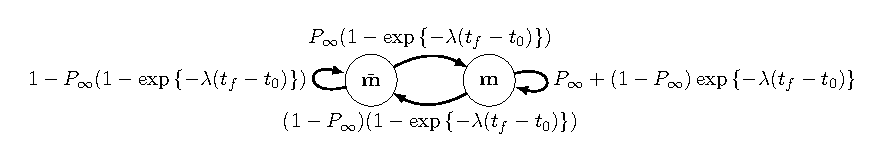
\includegraphics[width=\textwidth]{markov_diagram_continuous.pdf}
\caption{The continuous-time Markov process for a single binary cell occupancy is illustrated. As time progresses, this process degrades the cell slowly toward $P_\infty.$}
\label{fig:MarkovDegradeContinuous}
\end{figure}

Applying degradation is computationally-inexpensive due to the simplicity of \refeqn{CellDegradationScalar}. For an arbitrary positive fixed time step, $\exp\braces{-\lambda (t_f-t_0)}$ needs only be calculated once and is multiplied to every map cell. Similarly, the second term of \refeqn{CellDegradationScalar}, namely $P_\infty(1-\exp\braces{-\lambda (t_f-t_0)})$, is simply added to every cell. For grid cells with probabilities far from $P_\infty$, the times to converge to this final degraded value increase, shown in Fig. \ref{fig:DegradeExamples}. Slow convergence of cells with probabilities close to $0$ or $1$ allows the robots to stop viewing these cells, giving the robots opportunities to visit different regions before returning.

\begin{figure}
\centering
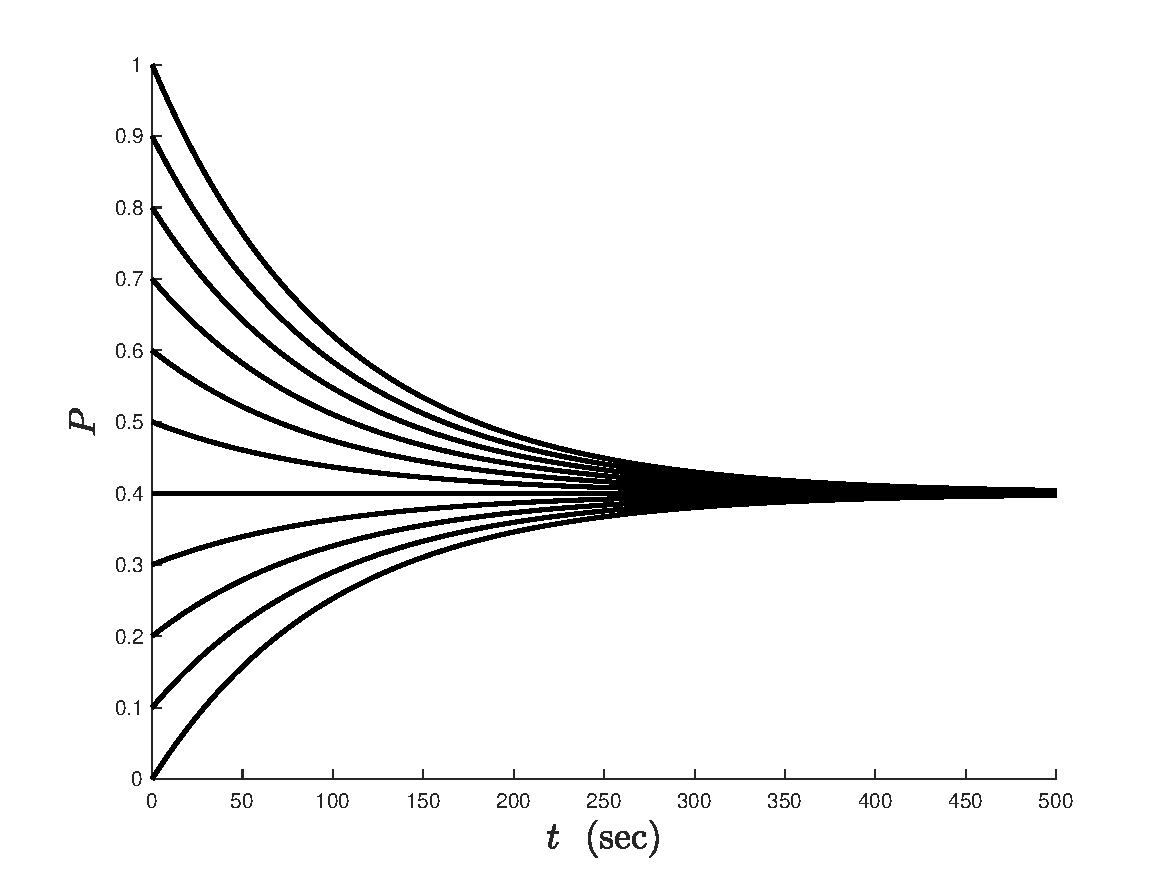
\includegraphics[width=\textwidth]{DegradeExamples.pdf}
\caption{The rate at which probabilities converge toward $P_\infty=0.4$ increases based on the difference magnitude of their initial values.}
\label{fig:DegradeExamples}
\end{figure}

In short, each grid cell is continuously degrading according to \refeqn{CellDegradationScalar} toward $P_\infty$. Only in the presence of measurements does the cell occupancy become well-known according to \refeqn{RayISMAnswer}--\refeqn{Unnormalized}. Cell degradation encourages the robot to revisit cells from the distant past using bidding-based multi-vehicle autonomous exploration to patrol the environment continuously. Adopting the receding horizon framework allows patrol to account for dynamic obstacles by quickly updating patrol strategies as map information changes.







\section{Single-Vehicle Exploration Experimental Results}
\label{sec:ExploreExperiment}

In this section, we present results from a single-vehicle autonomous exploration experiment. A robots builds a 3D map of its environment, which is projected onto a 2D map for exploration. Grid cell probabilities are determined from the onboard sensors without degradation, so this experiment focusses on exploration rather than patrol.

\subsection{Exploration Environment}

The U.S. Naval Research Laboratory (NRL) has a large experimental space for testing known as the Laboratory for Autonomous Systems Research (LASR). Here, we designed an experimental setup containing walls and objects to resemble a building floor plan. The perimeter walls were constructed with tan cardboard, which were suspended from $1$m tall stanchions, and an internal wall was built with gray metal sheeting mounted to $80/20$ supports~\cite{url_8020}. Additionally, a hard flooring reflected some florescent lighting above. The objects inside the experimental environment included various trash cans, desks, and chairs in addition to a few miscellaneous objects. The map size was selected to slightly exceed the volume of the experiment such that the the x-direction (positive east) spanned $0.5$m to $10.3$m, the y-direction (positive north) spanned $-8.3$m to $3.5$m, and the z-direction (positive vertically up) spanned $-0.15$m to $1.5$m. Two images of the experimental environment are displayed in Fig. \ref{fig:exp3DEnvironment}.

\begin{figure}[!t]
\centering
    	\begin{subfigure}[t]{0.95\columnwidth}
           	\centering
          	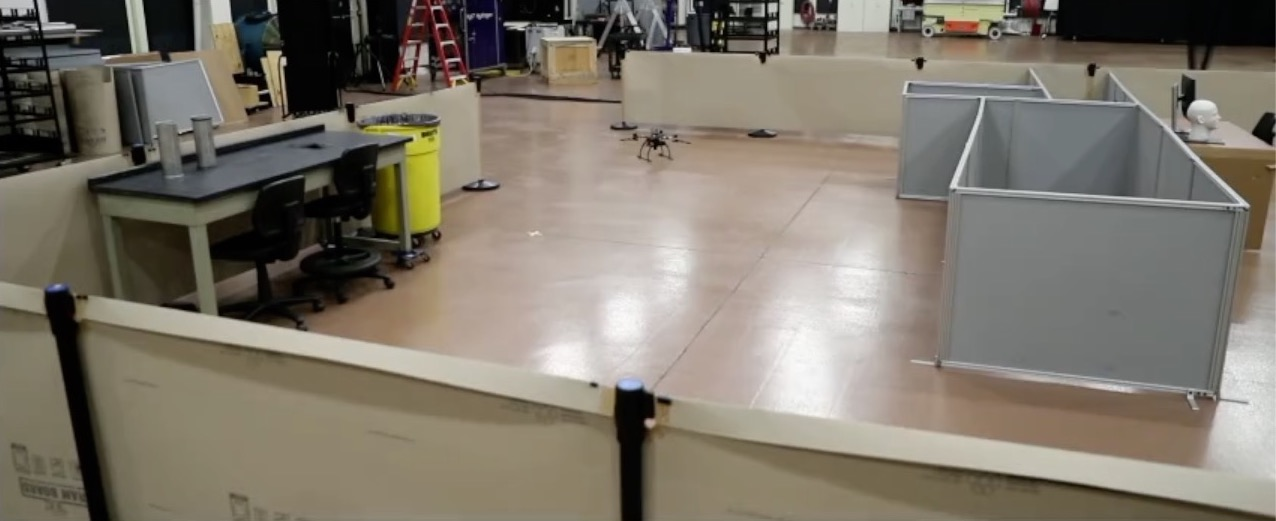
\includegraphics[width=\textwidth]{experiment_north.jpg}
        		\caption{North Region}
    	\end{subfigure}
    	\begin{subfigure}[t]{0.95\columnwidth}
	\vspace*{0.03\columnwidth}
           	\centering
          	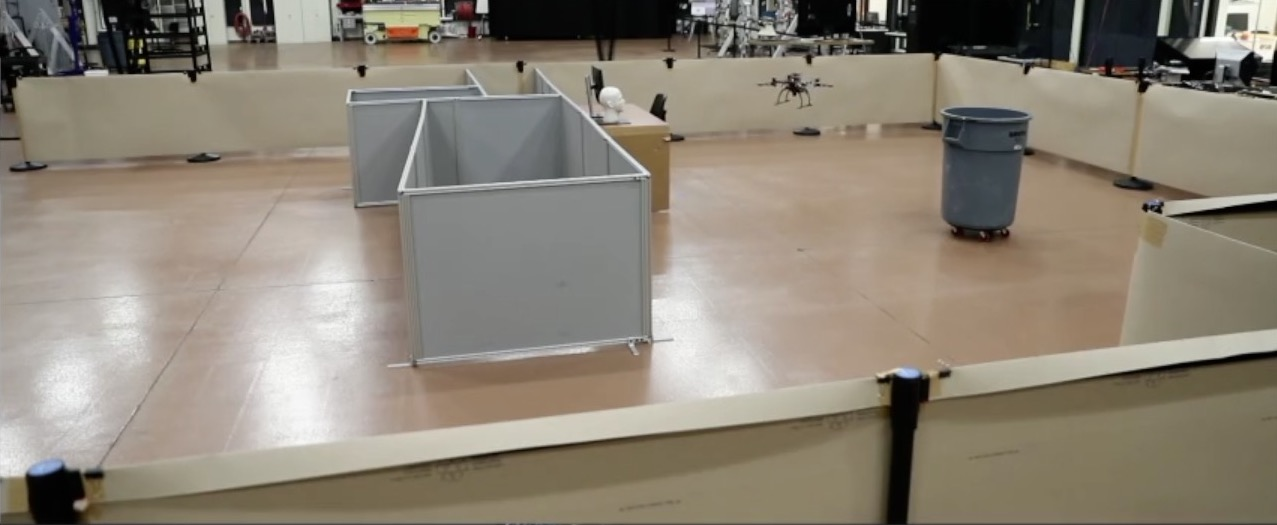
\includegraphics[width=\textwidth]{experiment_south.jpg}
        		\caption{South Region}
    	\end{subfigure}
	\caption{The 3D experimental environment is designed to resemble a large room within an office building. The walls are build from from cardboard suspended from stanchions and gray sheeting with $80/20$ supports, and miscellaneous objects are placed around the room as well.}
	\label{fig:exp3DEnvironment}
\end{figure}

Next we describe the key parameters used for mapping and exploration. The inverse sensor model \refeqn{RayISMAnswer}--\refeqn{Unnormalized} relies on the stochastic properties of two sensors, namely an Asus Xtion color IR depth sensor and a Hokuyo LIDAR. The Xtion and Hokuyo sensors are modeled using a modified version of the beam model for range finders~\cite{ThrBurFox05}. This includes uniform distribution for a phantom reading with probability $P_\text{rand}=0.1$ and a Gaussian distribution with probability $P_\text{hit}=0.9$. The Gaussian distribution corresponds to the desired case when the measurement $z$ correctly captures a particular cell at expected distance $\hat{z}$ with standard deviation $\sigma$. The total forward sensor model for the Xtion and Hokuyo is
\begin{align}
%p_\text{total}(z,z_\text{min},z_\text{max},\hat{z},\sigma)&=P_\text{rand}p_\text{rand}(z,z_\text{min},z_\text{max})+P_\text{hit}p_\text{hit}(z,\hat{z},\sigma),
&p_\text{total}=P_\text{rand}p_\text{rand}+P_\text{hit}p_\text{hit},
\\
&p_\text{rand}(z,z_\text{min},z_\text{max})=\frac1{z_\text{max}-z_\text{min}},
\\
&p_\text{hit}(z,\hat{z},\sigma)=\frac1{\sqrt{2\pi\sigma^2}}\exp\braces{\frac{(\hat{z}-z)^2}{{2\sigma^2}}},
\end{align}
such that $z_\text{min}=0.5$m and $z_\text{max}=4.0$m for both the Xtion and Hokuyo, and the standard deviations are $\sigma_\text{Xtion}=0.25$m and $\sigma_\text{Hokuyo}=0.1$m, respectively, which exceed their specified values to account for localization uncertainty and sensor distortion of the Xtion. These sensors update the probabilities of cubic 3D cells with edge length $\alpha=0.075$m and initial probability $P_\text{init}=0.1$.

The grid cells for the projected 2D map used during exploration are $3$ times the size, $0.225$m. Since this experiment does not require multi-vehicle patrol with a receding horizon framework, the bump function is simplified to decrease with increasing distance, similar to \refeqn{BumpFunDecreasing} following the structure of~\cite{Joh06} with $d_\text{max}>0$,
\begin{align}
\label{eqn:BumpFunRef}
\text{bump}(d)= 
\begin{cases}
    \exp\braces{{1-\frac1{1-(d/d_\text{max})^2}}},			& \text{if }0<d<d_\text{max}\\
    0,              				& \text{otherwise}
\end{cases},
\end{align}
such that $d_\text{max}$ is selected as the maximum cost map value. Then, $\text{bump}(d)$ is multiplied to \refeqn{expectedInfoGainRay} when finding optimal poses. The bump function prioritizes actions that improve the knowledge of the local surrounding space before distant traversals across the map.


\subsection{Hardware Structure}

Several components are used for localization, sensing, and actuation. A Vicon motion capture system provides the transformation between a reference frame fixed to the world and the moving vehicle. This transformation, along with fixed transformations between the robot body and the sensors, provides sufficient information for the transformation from the world to each sensor frame. The sensor readings from the Xtion and Hokuyo are transmitted from an NVidia Jetson TX2 onboard the vehicle (Fig. \ref{fig:QuadrotorHardware}). The sensor readings are received via WIFI on a host computer with an Intel Core i7-6800K CPU (12$\times$3.40GHz), which runs the mapping and exploration nodes. The host computer returns the exploration trajectories to the Jetson TX2 over WIFI. Then, the Jetson executes a nonlinear geometric flight controller~\cite{GooDaeLee13} onboard. With this configuration, large processing tasks are avoided onboard the robot.
		
\begin{figure}[!t]
\centering
    	\begin{subfigure}[t]{0.44\columnwidth}
           	\centering
          	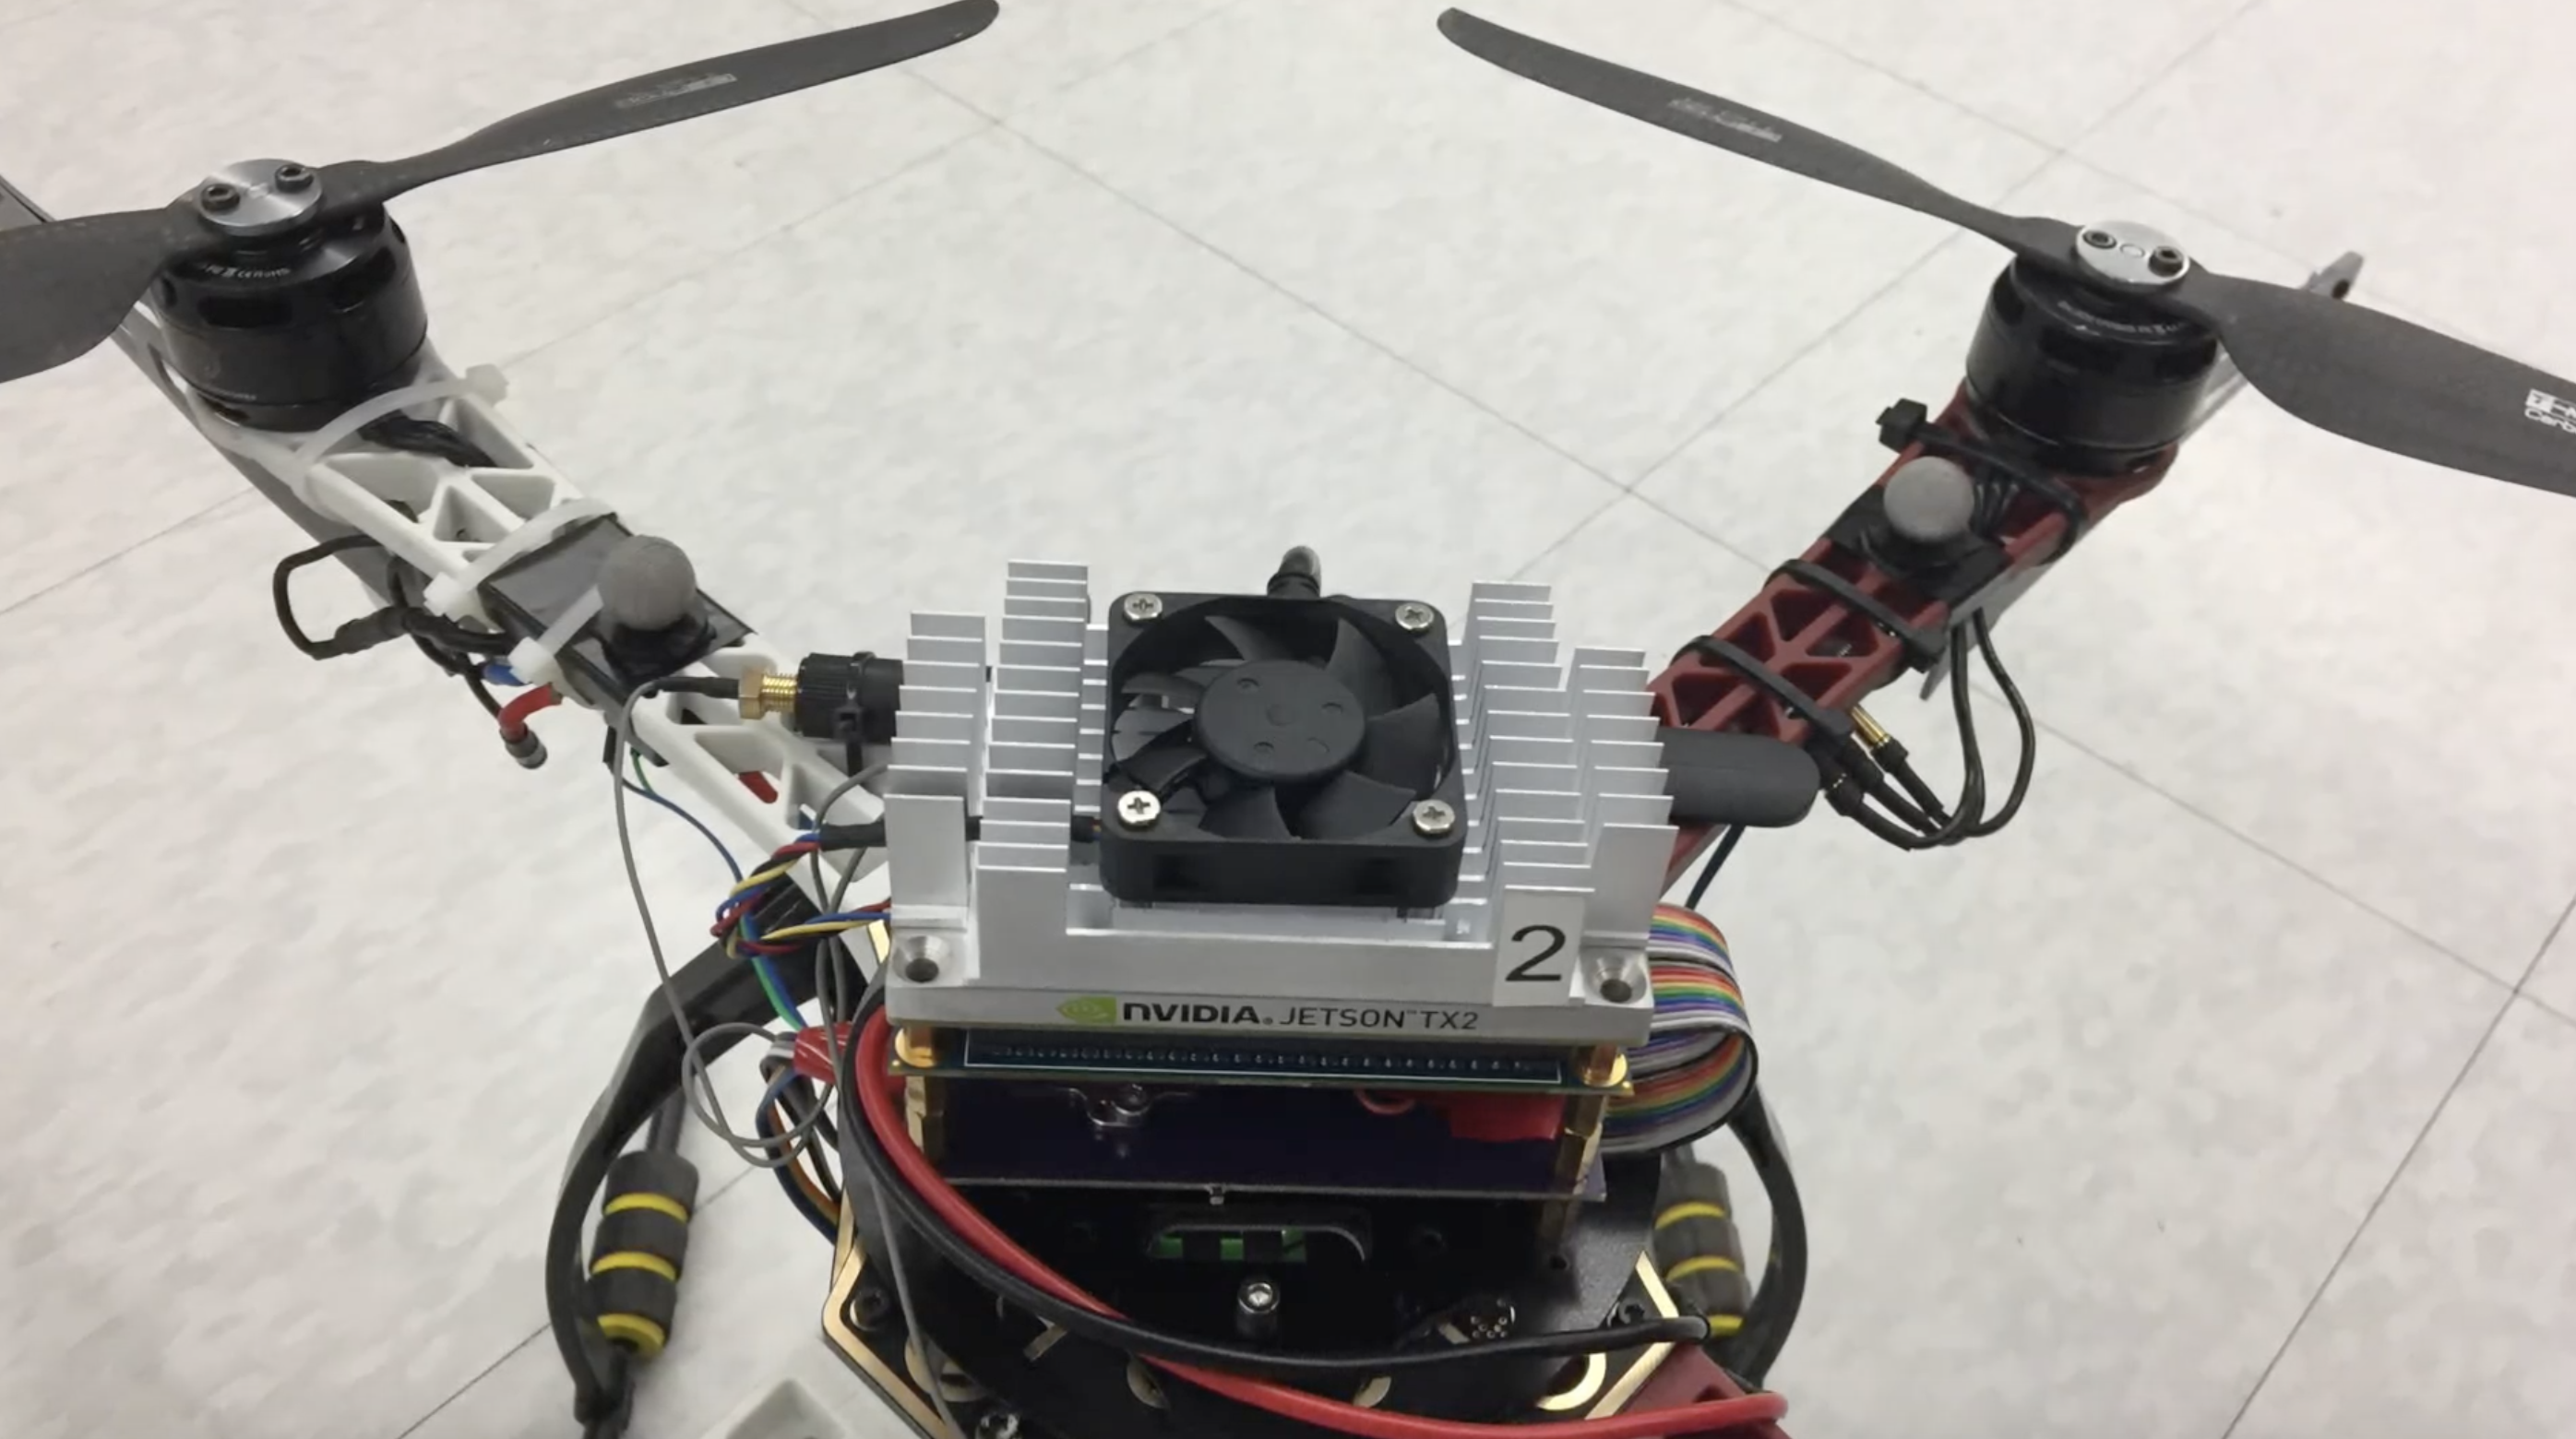
\includegraphics[width=\textwidth]{quad_top.png}
        		\caption{Quadrotor Top}
    	\end{subfigure}
	\hspace*{0.05\columnwidth}
    	\begin{subfigure}[t]{0.44\columnwidth}
           	\centering
          	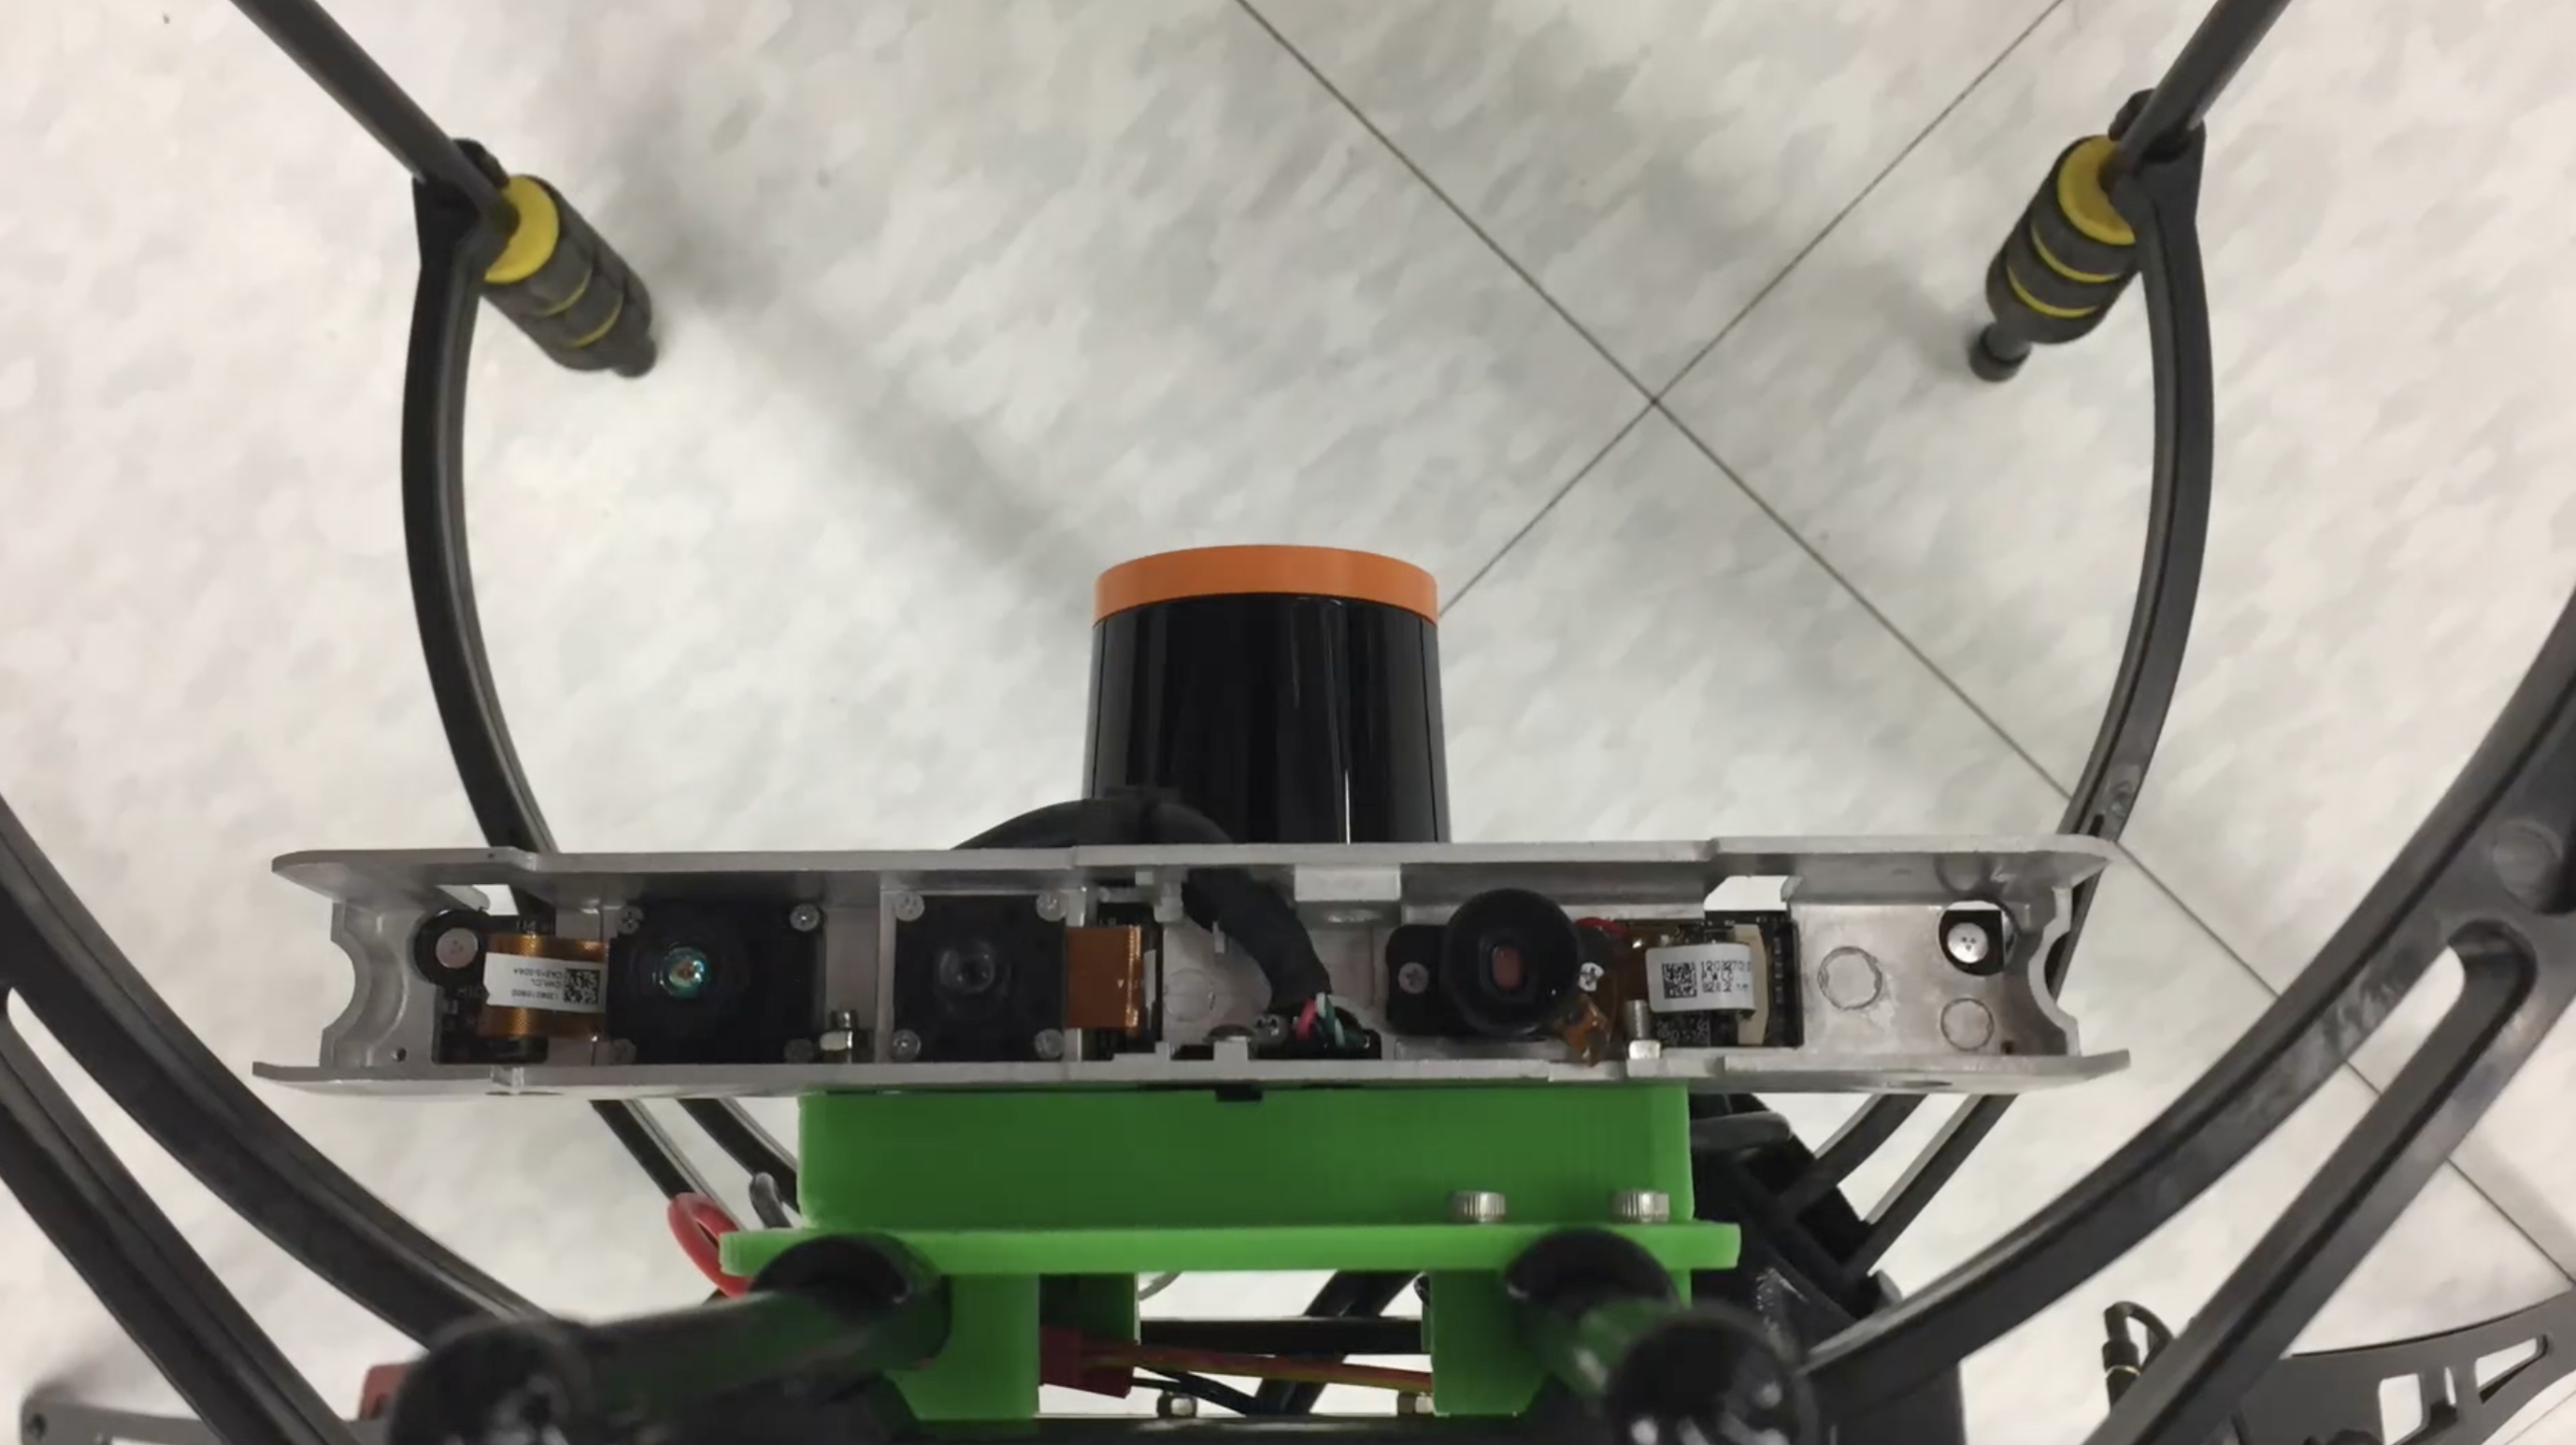
\includegraphics[width=\textwidth]{quad_bottom.png}
        		\caption{Quadrotor Bottom}
    	\end{subfigure}
	\caption{A Jetson TX2 (quadrotor top) streams depth measurements via WIFI from an Asus Xtion and Hokuyo LIDAR (quadrotor bottom). The host computer builds a 3D probabilistic occupancy grid map from these measurements. For autonomous exploration, the host computer designs exploration trajectories, which an onboard flight controller can track in real-time.}
	\label{fig:QuadrotorHardware}
\end{figure}

\subsection{Software Structure}

The software is developed using the Robot Operating System (ROS) framework for simple communication among the processes. The programs, referred to as \emph{nodes}, are primarily coded in C++ for efficiency, except a GUI and trivial message conversions, which use Python scripts. Additionally, a few launch, yaml, cfg scripts were used for running nodes and setting parameters.  

The first node creates a 3D probabilistic map. This node uses transform message filters (a variation of ROS message filters) to synchronize sensor transformations and associated sensor readings. This way, each measurement origin and direction is well-known, and is applied to ray casting in 3D, where all possible intersections between the measurement and grid cells are computed through geometry. Next, the cell probabilities along this ray are updated with the inverse sensor model \refeqn{RayISMAnswer}--\refeqn{Unnormalized}. The measurements are analyzed ray-by-ray, so any number of depth sensors with known stochastic properties may be used. For this experiment, the stochastic properties of the Xtion and Hokuyo are listed inside a yaml configuration file.


There are three nodes for exploration. The first node projects 3D grid cells onto a 2D map according to \refeqn{Proj2DMapComb}, then publishes this 2D map for visualization and further analysis. The second node subscribes to the 2D map for Dijkstra's search and information gain optimization. This node produces path messages, which consist of desired poses $0.01$sec apart for visualization using the ROS package, Rviz. Finally, an additional node sends the desired pose at the current time to the geometric nonlinear controller~\cite{GooDaeLee13} onboard the robot.

\subsection{Experimental Results}
                
The quadrotor takes off, completes a rotation to understand its immediate surroundings, then explores the space over $2$ minutes and $47$ seconds. Fig. \ref{fig:exp3DMap} shows the probabilistic 3D map generated in real-time at four selected times, and the corresponding 2D projected maps (x-direction upward) are illustrated in Fig. \ref{fig:exp2DMap}, where arrows represent pose candidates and a trajectory is shown to the optimal pose. Fig. \ref{fig:expH} shows the total map entropy decreasing over the experiment duration. A video of the experiment can be found at \href{https://www.youtube.com/watch?v=I_1rXV2XRqk}{https://www.youtube.com/watch?v=I\_1rXV2XRqk}.

% trim={<left> <lower> <right> <upper>}

\begin{figure}[!t]
\centering
    	\begin{subfigure}[t]{0.95\columnwidth}
           	\centering
          	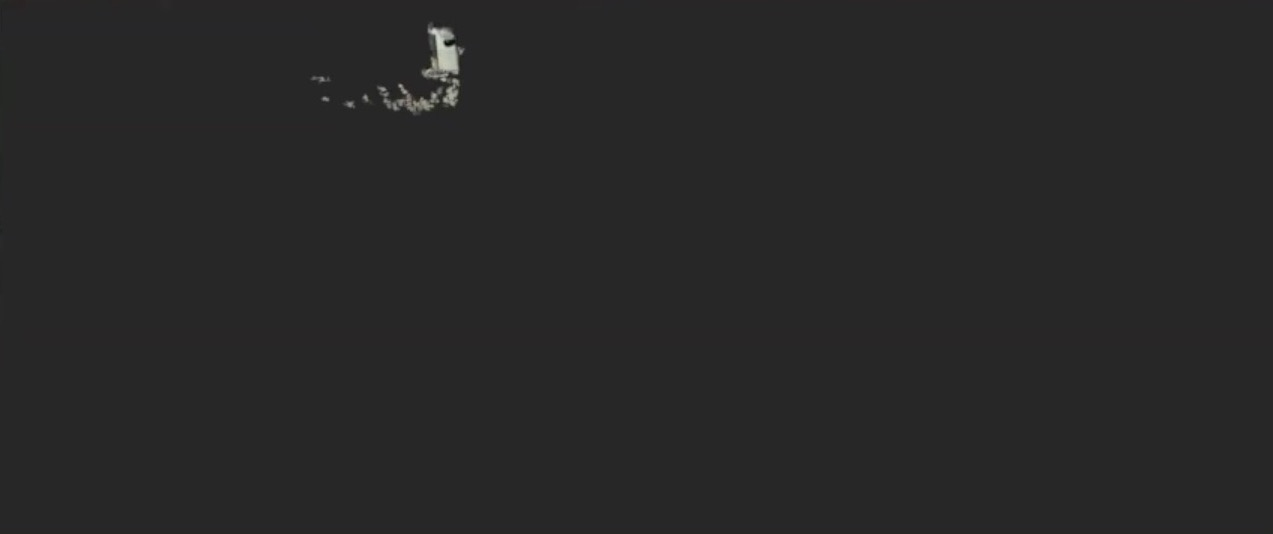
\includegraphics[width=\textwidth]{experiment_ogm3D_0min.jpg}
        		\caption{$0$ min}
    	\end{subfigure}
    	\begin{subfigure}[t]{0.95\columnwidth}
		\vspace*{0.03\columnwidth}
           	\centering
          	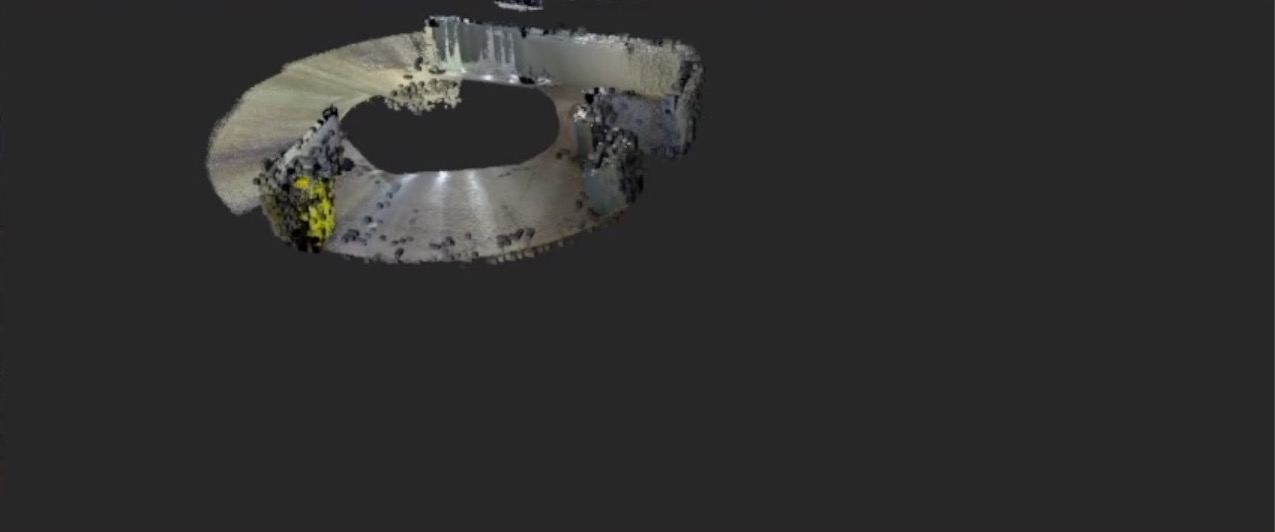
\includegraphics[width=\textwidth]{experiment_ogm3D_1min.jpg}
        		\caption{$1$ min}
    	\end{subfigure}
    	\begin{subfigure}[t]{0.95\columnwidth}
	\vspace*{0.03\columnwidth}
           	\centering
          	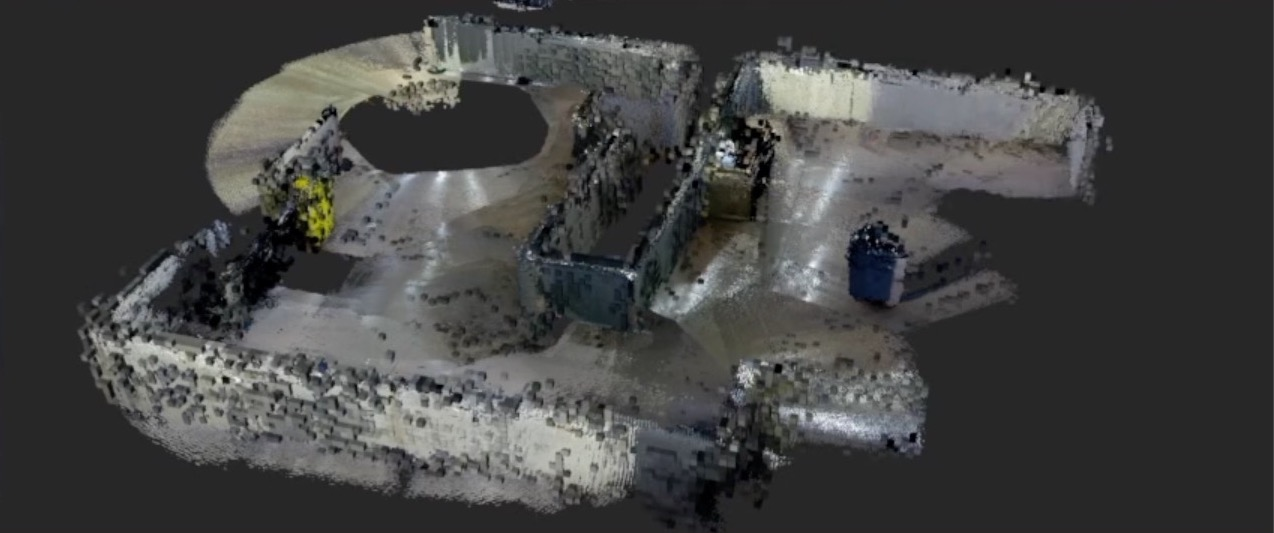
\includegraphics[width=\textwidth]{experiment_ogm3D_2min.jpg}
        		\caption{$2$ min}
    	\end{subfigure}
    	\begin{subfigure}[t]{0.95\columnwidth}
	\vspace*{0.03\columnwidth}
           	\centering
          	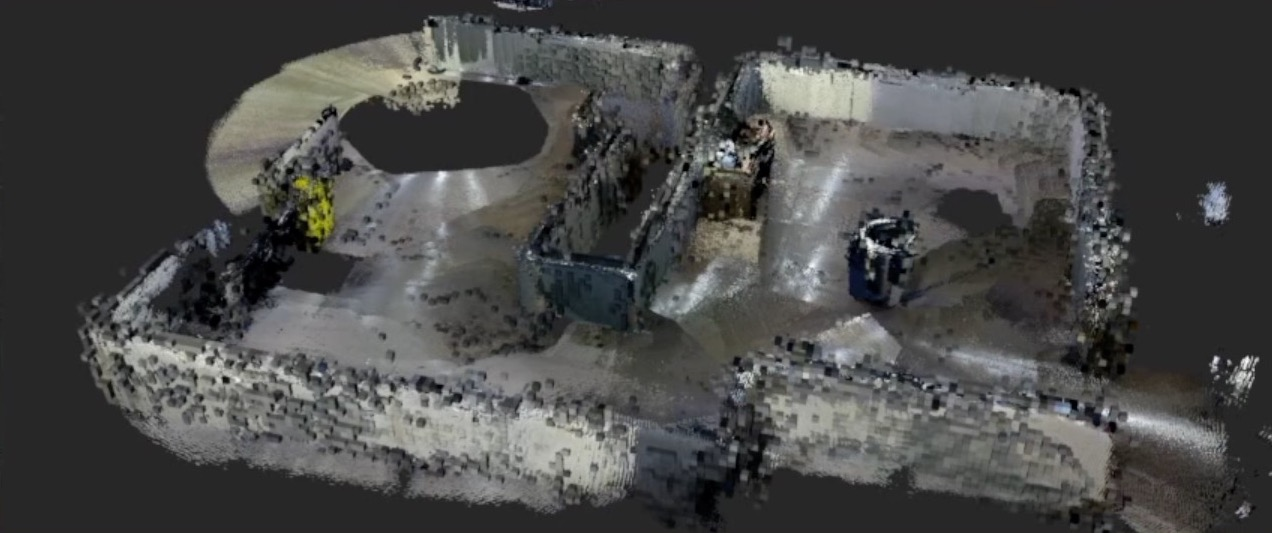
\includegraphics[width=\textwidth]{experiment_ogm3D_2min47sec.jpg}
        		\caption{$2$ min $47$ sec (end)}
    	\end{subfigure}
	\caption{The 3D occupancy grid map is overlaid with point cloud measurements. The map probabilities directly rely on the Xtion and Hokuyo measurements and the sensor stochastic properties.}
	\label{fig:exp3DMap}
\end{figure}

\begin{figure}[!t]
\centering
    	\begin{subfigure}[t]{0.44\columnwidth}
           	\centering
          	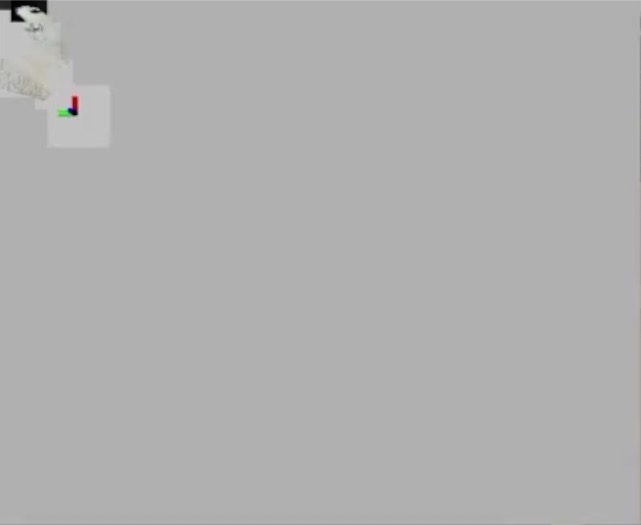
\includegraphics[width=\textwidth]{experiment_0min_2D.jpg}
        		\caption{$0$ min}
    	\end{subfigure}
    	\begin{subfigure}[t]{0.44\columnwidth}
           	\centering
          	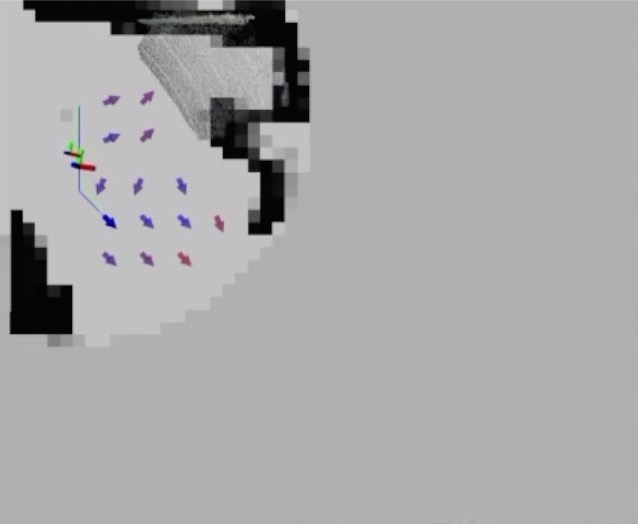
\includegraphics[width=\textwidth]{experiment_1min_2D.jpg}
        		\caption{$1$ min}
    	\end{subfigure}
    	\begin{subfigure}[t]{0.44\columnwidth}
           	\centering
          	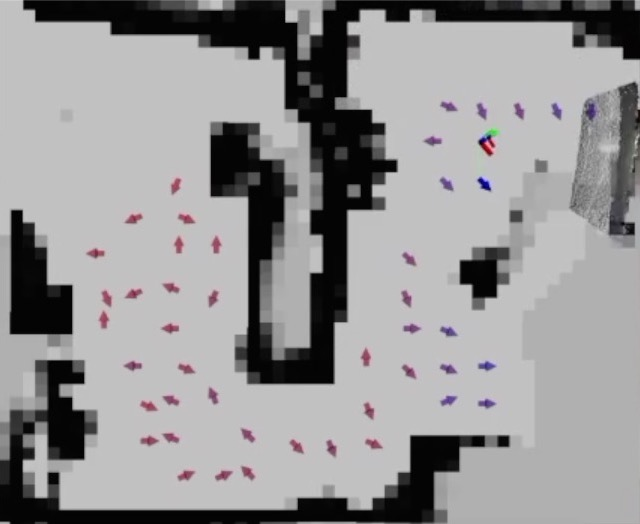
\includegraphics[width=\textwidth]{experiment_2min_2D.jpg}
        		\caption{$2$ min}
    	\end{subfigure}
    	\begin{subfigure}[t]{0.44\columnwidth}
           	\centering
          	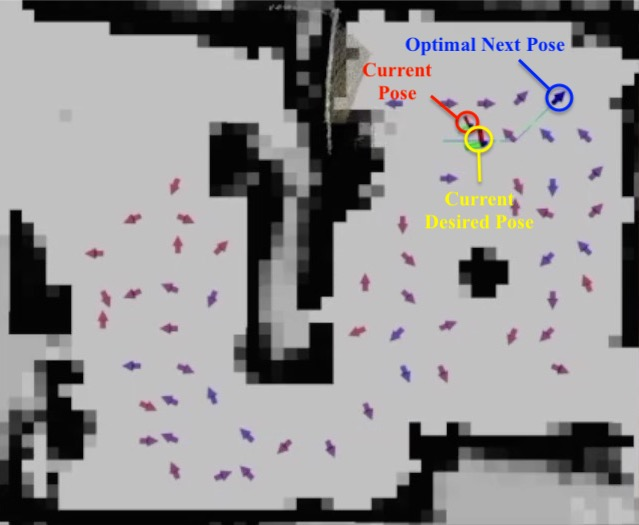
\includegraphics[width=\textwidth]{experiment_2min47sec_2D_labeled.jpeg}
        		\caption{$2$ min $47$ sec (end)}
    	\end{subfigure}
	\caption{The 2D projected map is easily produced in real-time. Candidate future poses, shown by arrows, have more blue color for larger objective functions, found with expected information gains and travel distances. Collision-free waypoints (blue line) serve as input to a constrained polynomial least-squares path (light green curve) for the robot controller to follow, where the desired pose (large axes) is tracked by the onboard controller from the current robot pose (small axes).}
	\label{fig:exp2DMap}
\end{figure}

\begin{figure}[!t]
	\centering
	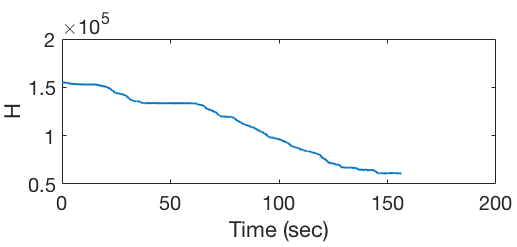
\includegraphics[width=0.85\textwidth]{entropy_experiment_aspect3by1.png}
	\caption{Map entropy decreases as the robot explores and captures more of the experimental environment.}
	\label{fig:expH}
\end{figure}

The robot is able to produce a 3D occupancy grid in under $3$ minutes without a human providing a trajectory. The 3D map can be easily interpreted by a human, and provides sufficient information in real-time for autonomous exploration. Optimal poses and collision-free exploration trajectories are calculated by the exploration node in under $1$ second. These quick decisions are vital to the autonomous exploration performance since the map is initially uncertain.

The projected map used for both collision and exploration has several benefits. The robot measures walls and objects with the 3D map, and nicely represents these as occupied spaces with the 2D projected map. Additionally, the exploration computation is low, allowing only for brief hover periods (less than $1$ second) between trajectories. However, the robot exploration does not consider those cells far below the robot, particularly those near the ground. As a result, some floor regions are not captured by the 3D occupancy grid even though cells above the floor are well-known.


\section{Multi-Vehicle Patrol Simulation Results}
\label{sec:PatrolSimulation}

In this section, we present a multi-vehicle exploration and patrol simulation. The environment is much larger, and the rate of measurements is increased with six active sensors, presenting several computational challenges. Furthermore, a human is walking around the space, unknown to the cooperating robots, requiring a receding horizon framework to avoid collisions.

\subsection{Simulated Environment}

Several parameters used during the multi-vehicle patrol simulation are identical to those of the prior section, with a few key differences relating specifically to the changed simulated environment and the bump function. There are three quadrotors with identical sensors as the last section cooperatively bidding on future poses in a much larger space. The environment is based on The George Washington University's (GWU) Science and Engineering Hall (SEH) floor plan, shown in Fig. \ref{fig:SEHEnvironment}. The map limits are much larger to accommodate the space, modified to $-55.0$m to $55.0$m in the x- and y-directions, and $0.0$m to $1.5$m in the z-direction, producing a total of $45,255,504$ grid cells with edge length $0.075$m (dimensioned $1468\times1468\times21$). For the bump function, $f_\text{max}=1$, $f_\text{far}=0.1$, and $\beta=0.01$ are chosen. For bidding $\rho_\text{max}=3.0$m is chosen.


\subsection{Software Structure}

The same ROS structure is largely used from the prior section, with key differences relating to process scalability and increased functionality with three vehicles patrolling the space. The mapping node, which computes 3D mapping probabilities, is modified in two ways: first, a thread is allocated to each sensor to update the map due to the much greater number of measurements, now originating from an Asus Xtion and Hokuyo LIDAR from each of three robots (six sensor scans total). An additional thread handles cell degradation with $\lambda=1\times10^{-3}$, which corresponds to a cell half life of roughly $11.5$ minutes; if this time passes since a measurement captures a cell, the occupancy probability will be halfway between its value $11.5$ minutes ago and $P_\infty=P_\text{init}=0.1$. While degrading cells with \refeqn{CellDegradationScalar} is inexpensive, degradation must cycle through all cells, which can be costly with a map containing over $45$ million cells. 

The exploration node is modified as well to handle a larger map with degrading cell probabilities. This node is composed of four threads. The first thread updates a local copy of the 3D occupancy grid map by subscribing to map changes from each sensor scan, which updates a small portion of the 2D projected map each time. This is accomplished by finding a rectangular prism of the minimum and maximum limits of cells that may have changed during a particular measurement scan update. Publishing and subscribing to map changes provides an efficient means to transfer mapping information, independent of map size. This way, robots understand their immediate surroundings quickly. The second node subscribes to the full 3D map, acquiring just the memory necessary to update the entire 2D projected occupancy grid map. This process is slower than the first thread due to the large 3D map size, but vital for tracking degradation of grid cells far from the current robot positions. The third thread runs the bidding-based information gain and travel distance optimizations following the receding horizon framework. During this thread, a local copy of the projected 2D map is locked to ensure a fair bidding process. The final thread simply broadcasts the projected map for visualization. The node for interpreting trajectory commands is the same as that of the prior section, and is run three times (once for each robot) in parallel. In short, this node structure is capable of multi-vehicle exploration and patrol with a receding horizon, and updates all map cell probabilities, prioritizing those close to the current robot positions.

\begin{figure}[!t]
\centering
    	\begin{subfigure}[t]{0.4\columnwidth}
           	\centering
          	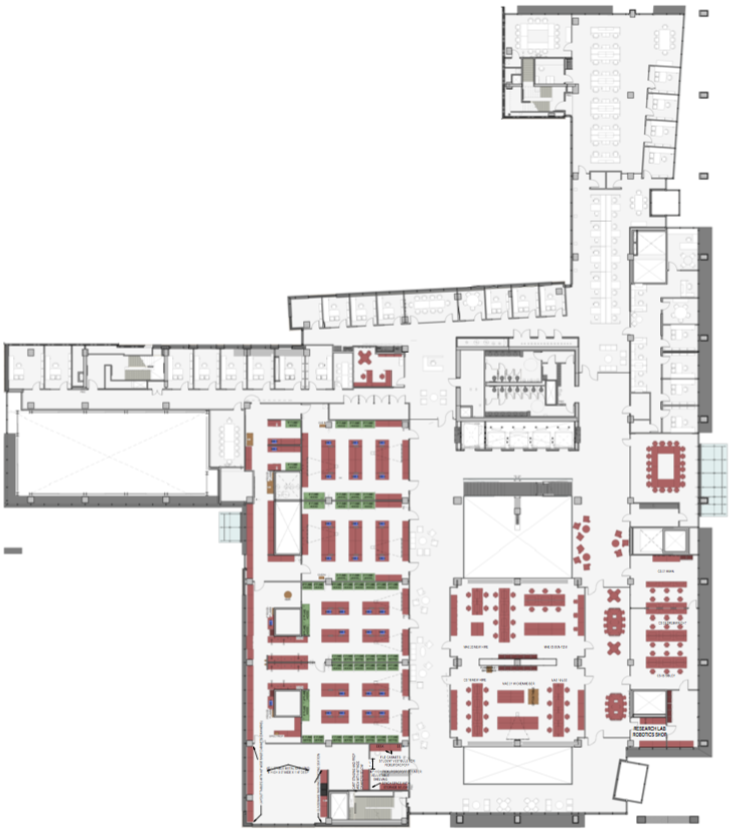
\includegraphics[width=\textwidth]{SEH_cropped.png}
        		\caption{Floor Plan}
    	\end{subfigure}
	\hspace*{0.1\textwidth}
    	\begin{subfigure}[t]{0.4\columnwidth}
           	\centering
          	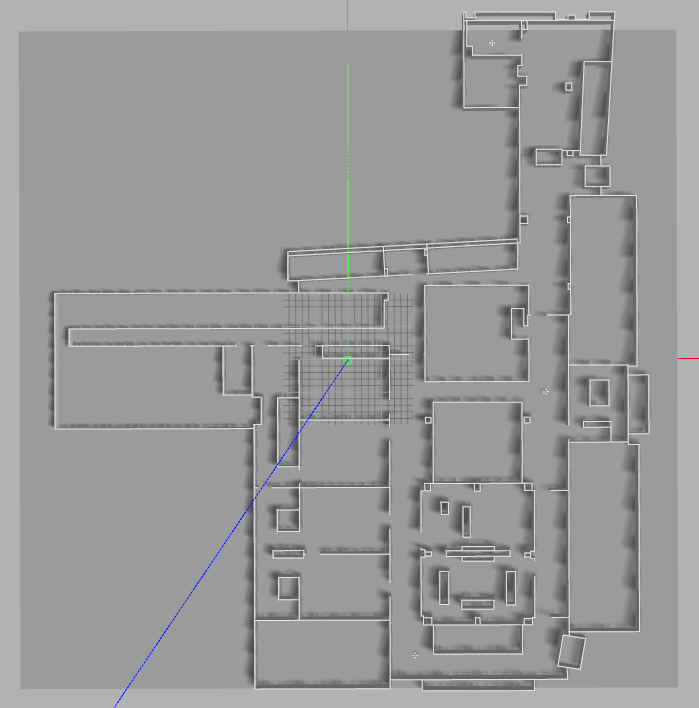
\includegraphics[width=\textwidth]{gazeboSEH.png}
        		\caption{Gazebo Model}
    	\end{subfigure}
	\caption{The SEH second floor plan (about $15,000$ sqft) is reconstructed with a Gazebo simulation environment.}
	\label{fig:SEHEnvironment}
\end{figure}


\subsection{Simulated Results}

In the simulation, three quadrotors explore and patrol the simulated environment of The George Washington University's (GWU) Science and Engineering Hall (SEH) for $15$ minutes while taking measurements. Initially, the robots are given no information about the environment except that their immediate surroundings are free. Unknown to the robot team, a simulated human walks in a rectangular repeated pattern at $0.5$ m/s. The 3D occupancy grid maps are shown in Fig. \ref{fig:sim3DMap}, and the corresponding 2D projected maps for exploration are shown in Fig. \ref{fig:sim2Dmaps}. The full video of both maps is available at \href{https://youtu.be/bsLG2romP_8}{https://youtu.be/bsLG2romP\_8}.

\begin{figure}[!t]
\centering
    	\begin{subfigure}[t]{0.38\columnwidth}
           	\centering
          	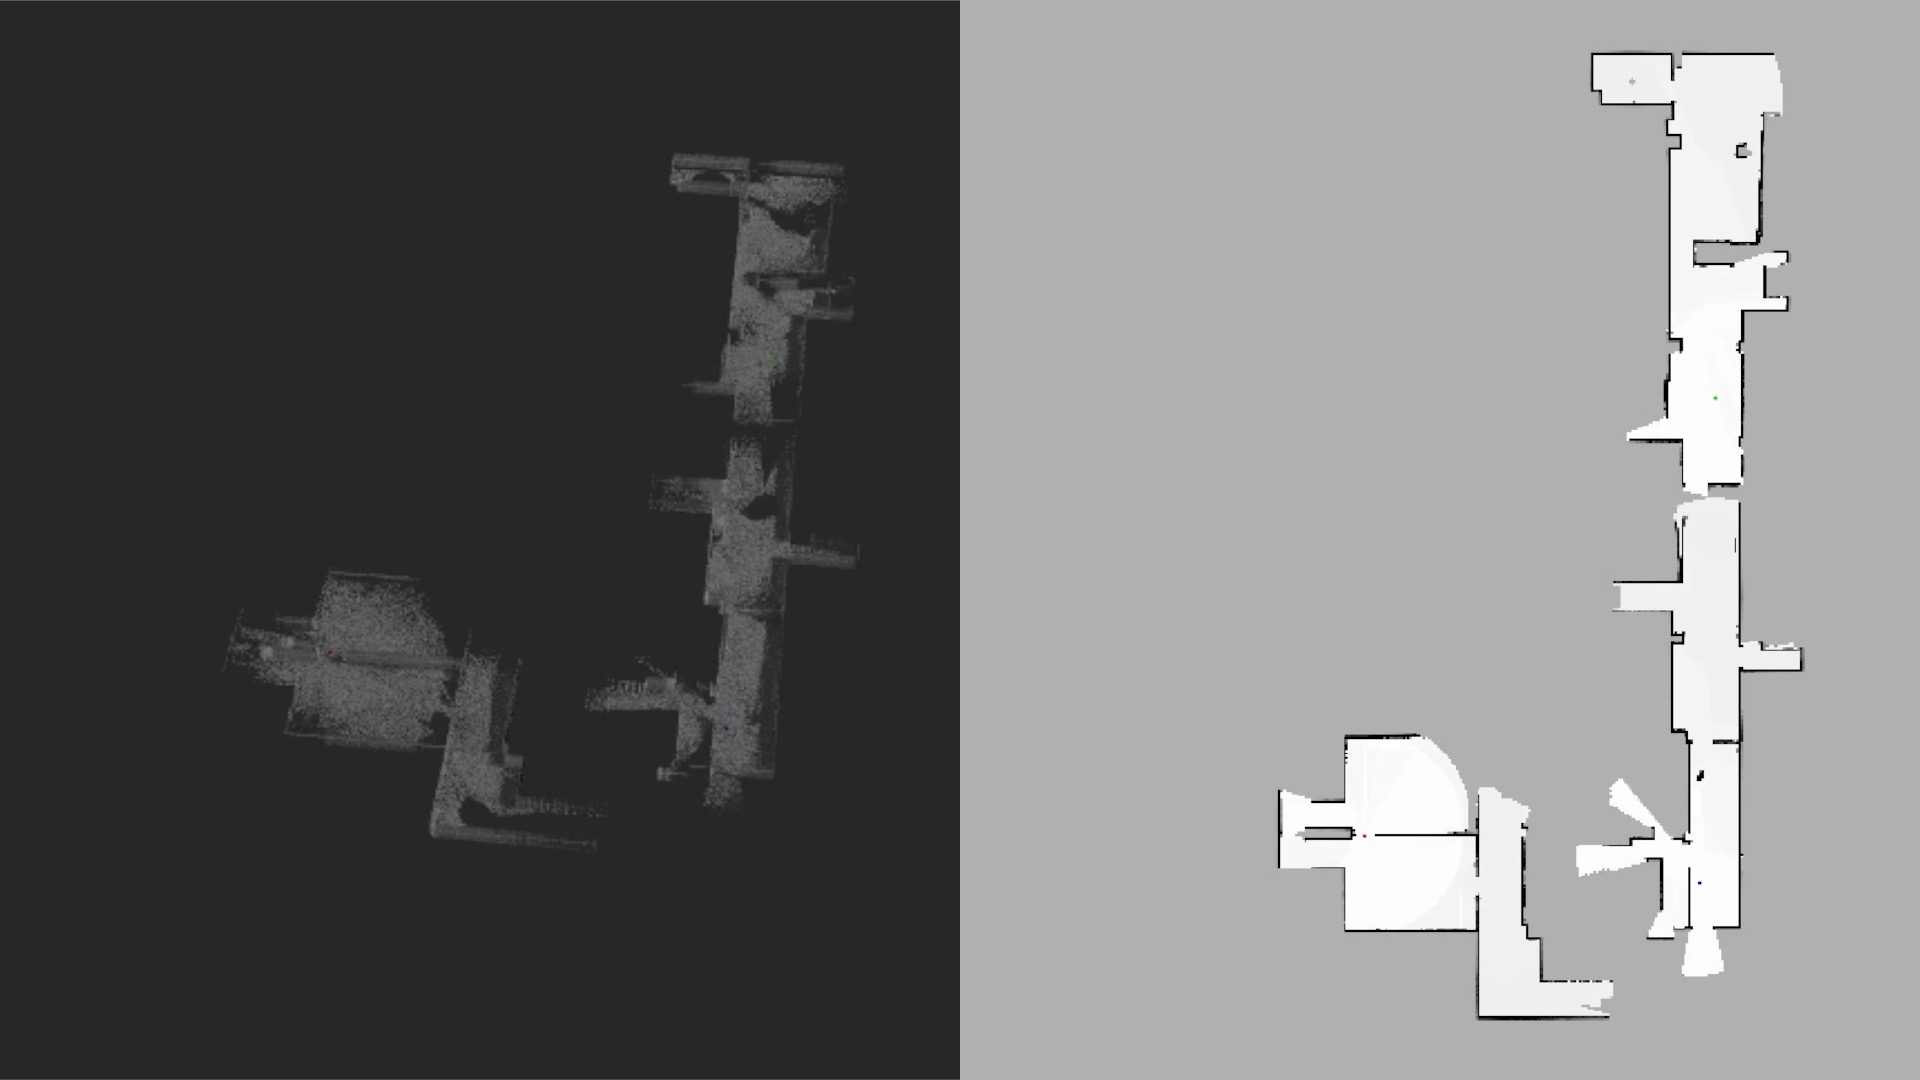
\includegraphics[trim={0cm 0cm 35cm 0cm}, clip, width=\textwidth]{Patrol_Split_Screen_1min.jpg}
        		\caption{$1$ min}
		\vspace*{0.05\textwidth}
    	\end{subfigure}
	\hspace*{0.05\textwidth}
    	\begin{subfigure}[t]{0.38\columnwidth}
           	\centering
          	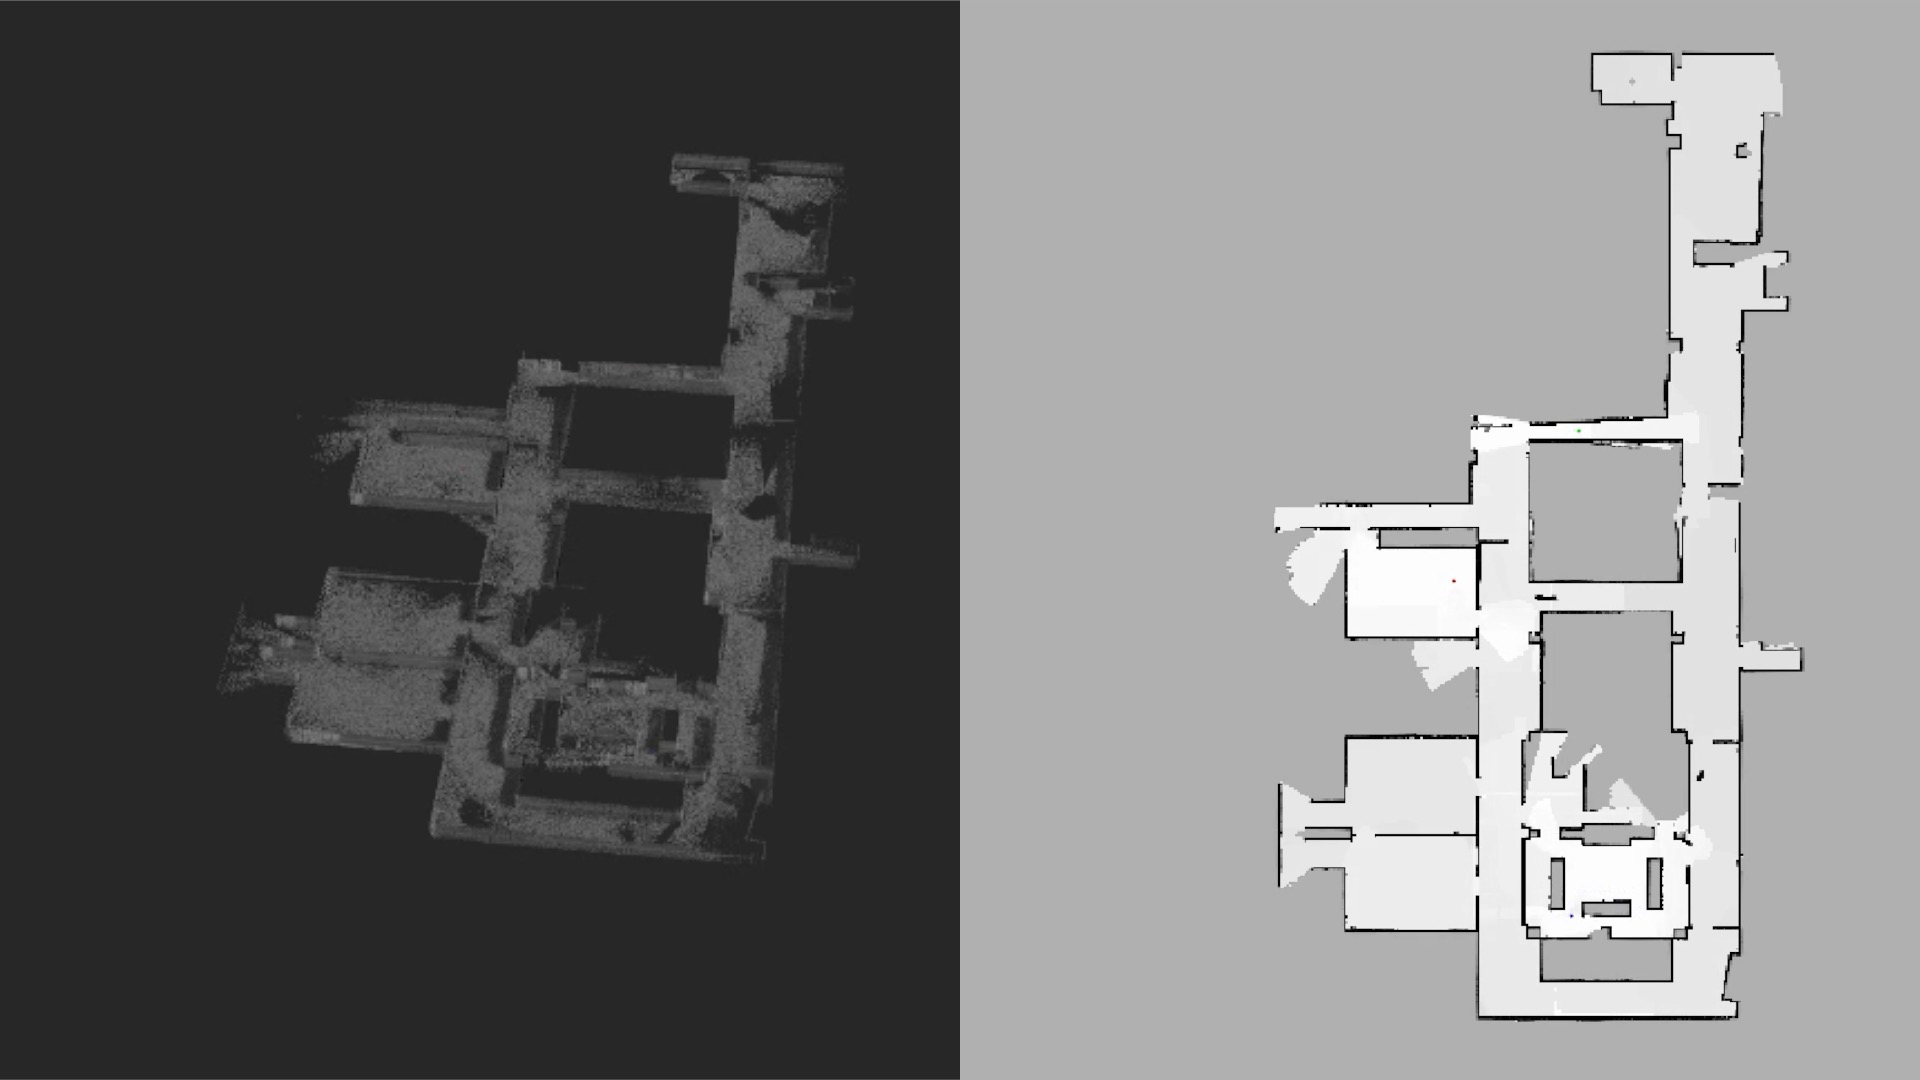
\includegraphics[trim={0cm 0cm 35cm 0cm}, clip, width=\textwidth]{Patrol_Split_Screen_3min.jpg}
        		\caption{$3$ min}
		\vspace*{0.05\textwidth}
    	\end{subfigure}
	\begin{subfigure}[t]{0.38\columnwidth}
           	\centering
          	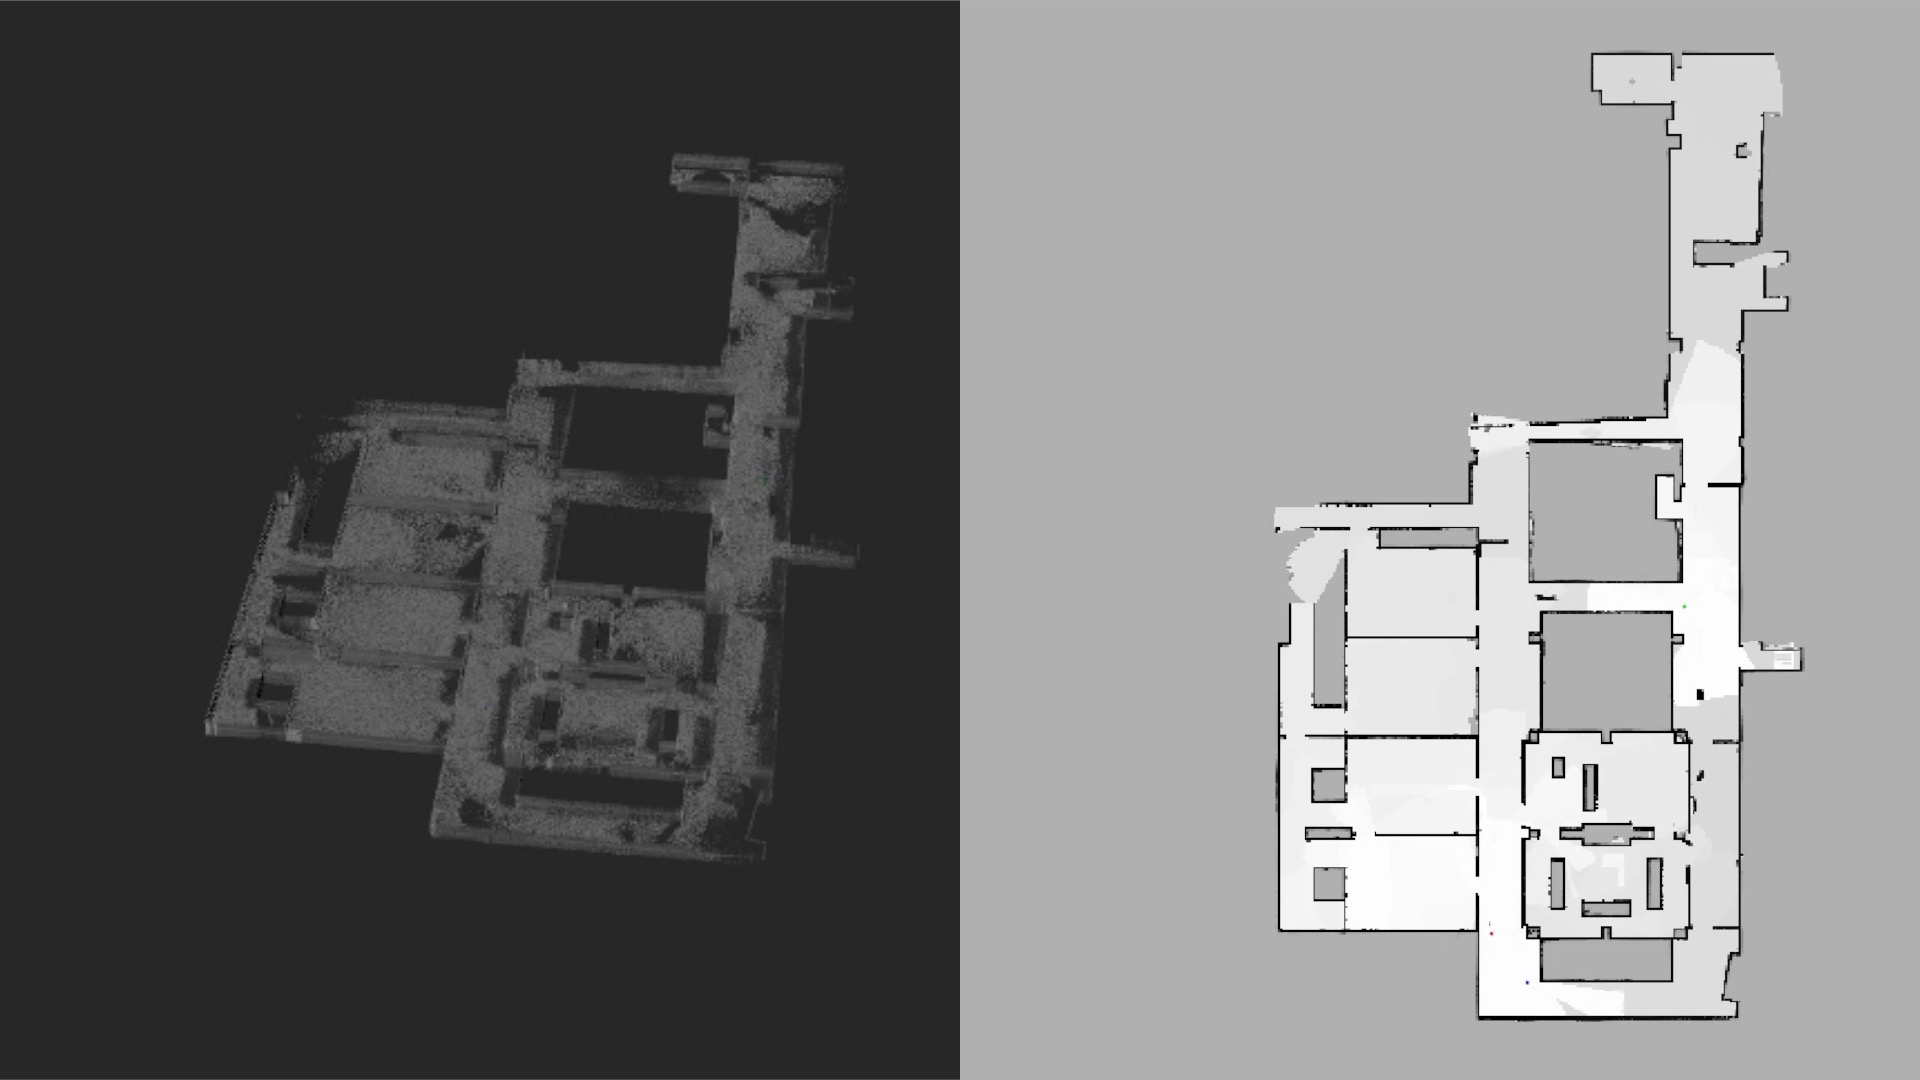
\includegraphics[trim={0cm 0cm 35cm 0cm}, clip, width=\textwidth]{Patrol_Split_Screen_5min.jpg}
        		\caption{$5$ min}
		\vspace*{0.05\textwidth}
    	\end{subfigure}
	\hspace*{0.05\textwidth}
    	\begin{subfigure}[t]{0.38\columnwidth}
           	\centering
          	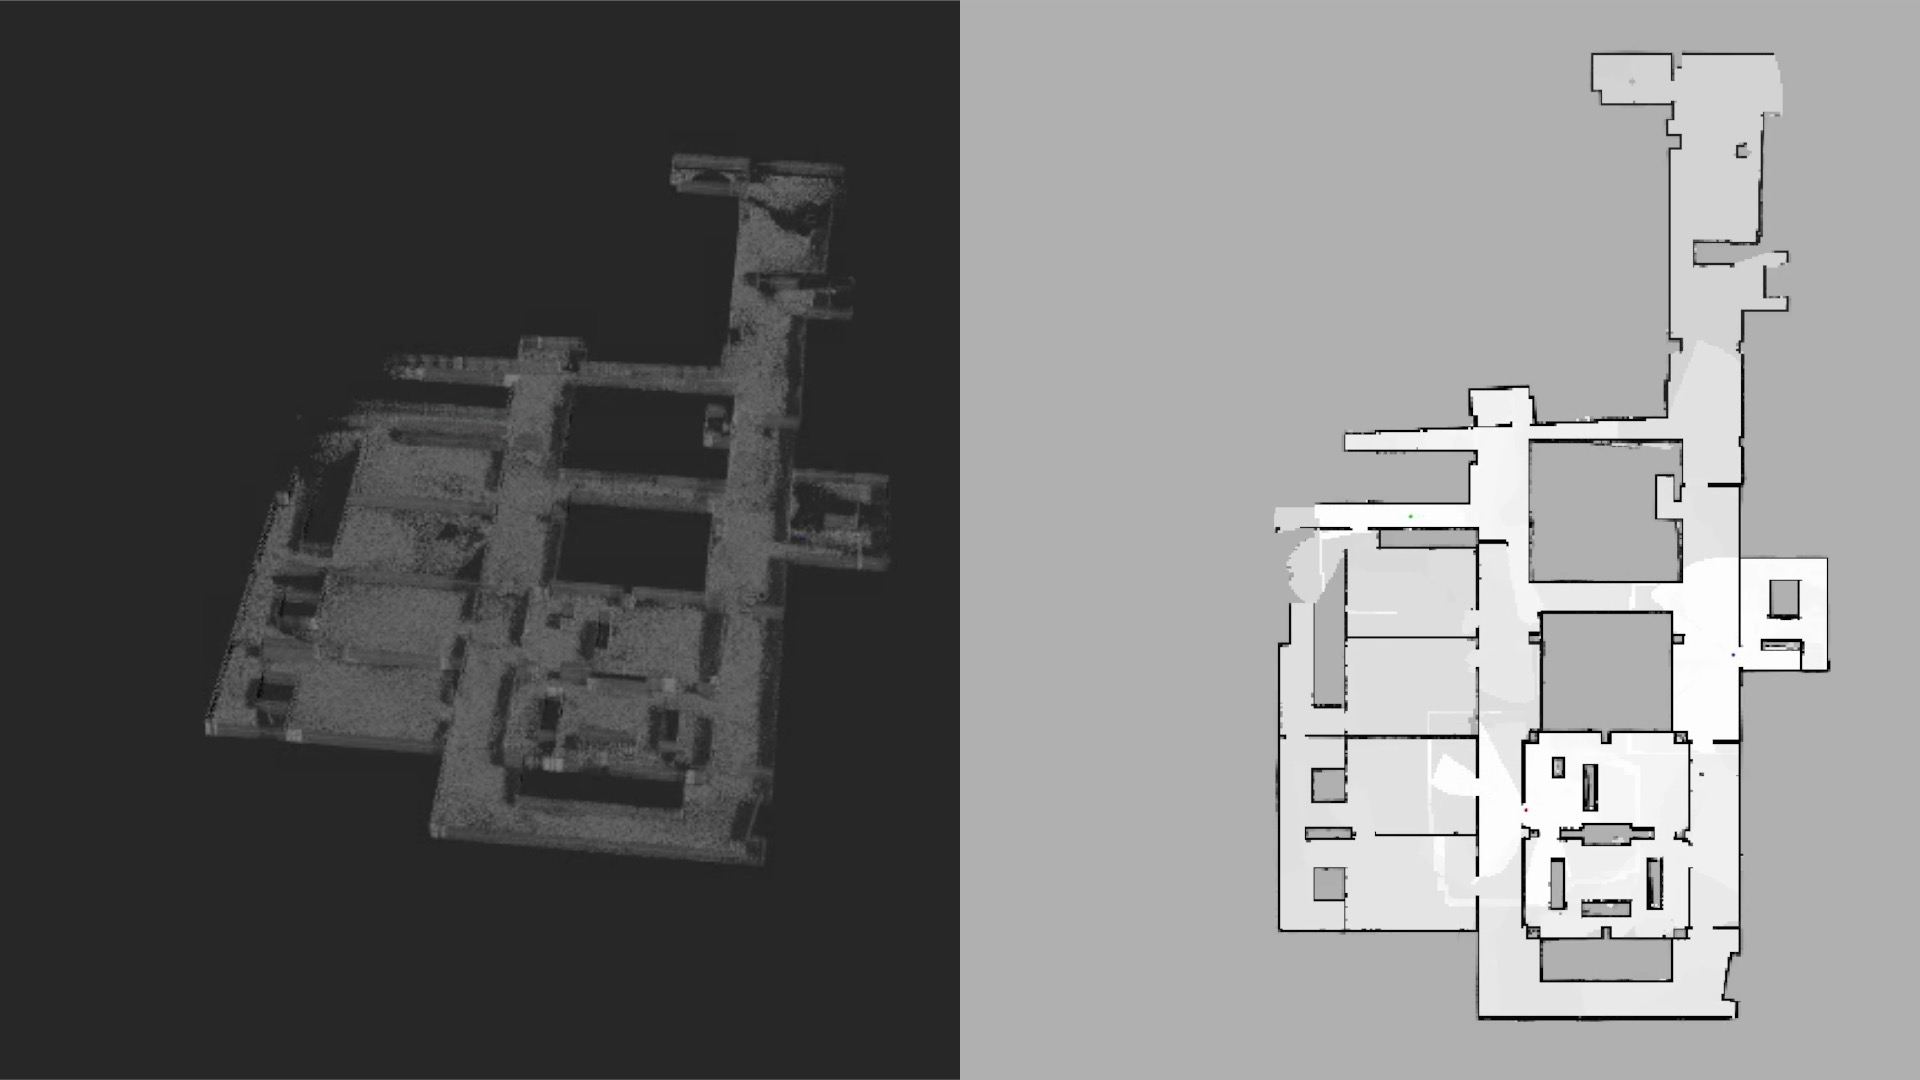
\includegraphics[trim={0cm 0cm 35cm 0cm}, clip, width=\textwidth]{Patrol_Split_Screen_7min.jpg}
        		\caption{$7$ min}
		\vspace*{0.05\textwidth}
    	\end{subfigure}
    	\begin{subfigure}[t]{0.38\columnwidth}
           	\centering
          	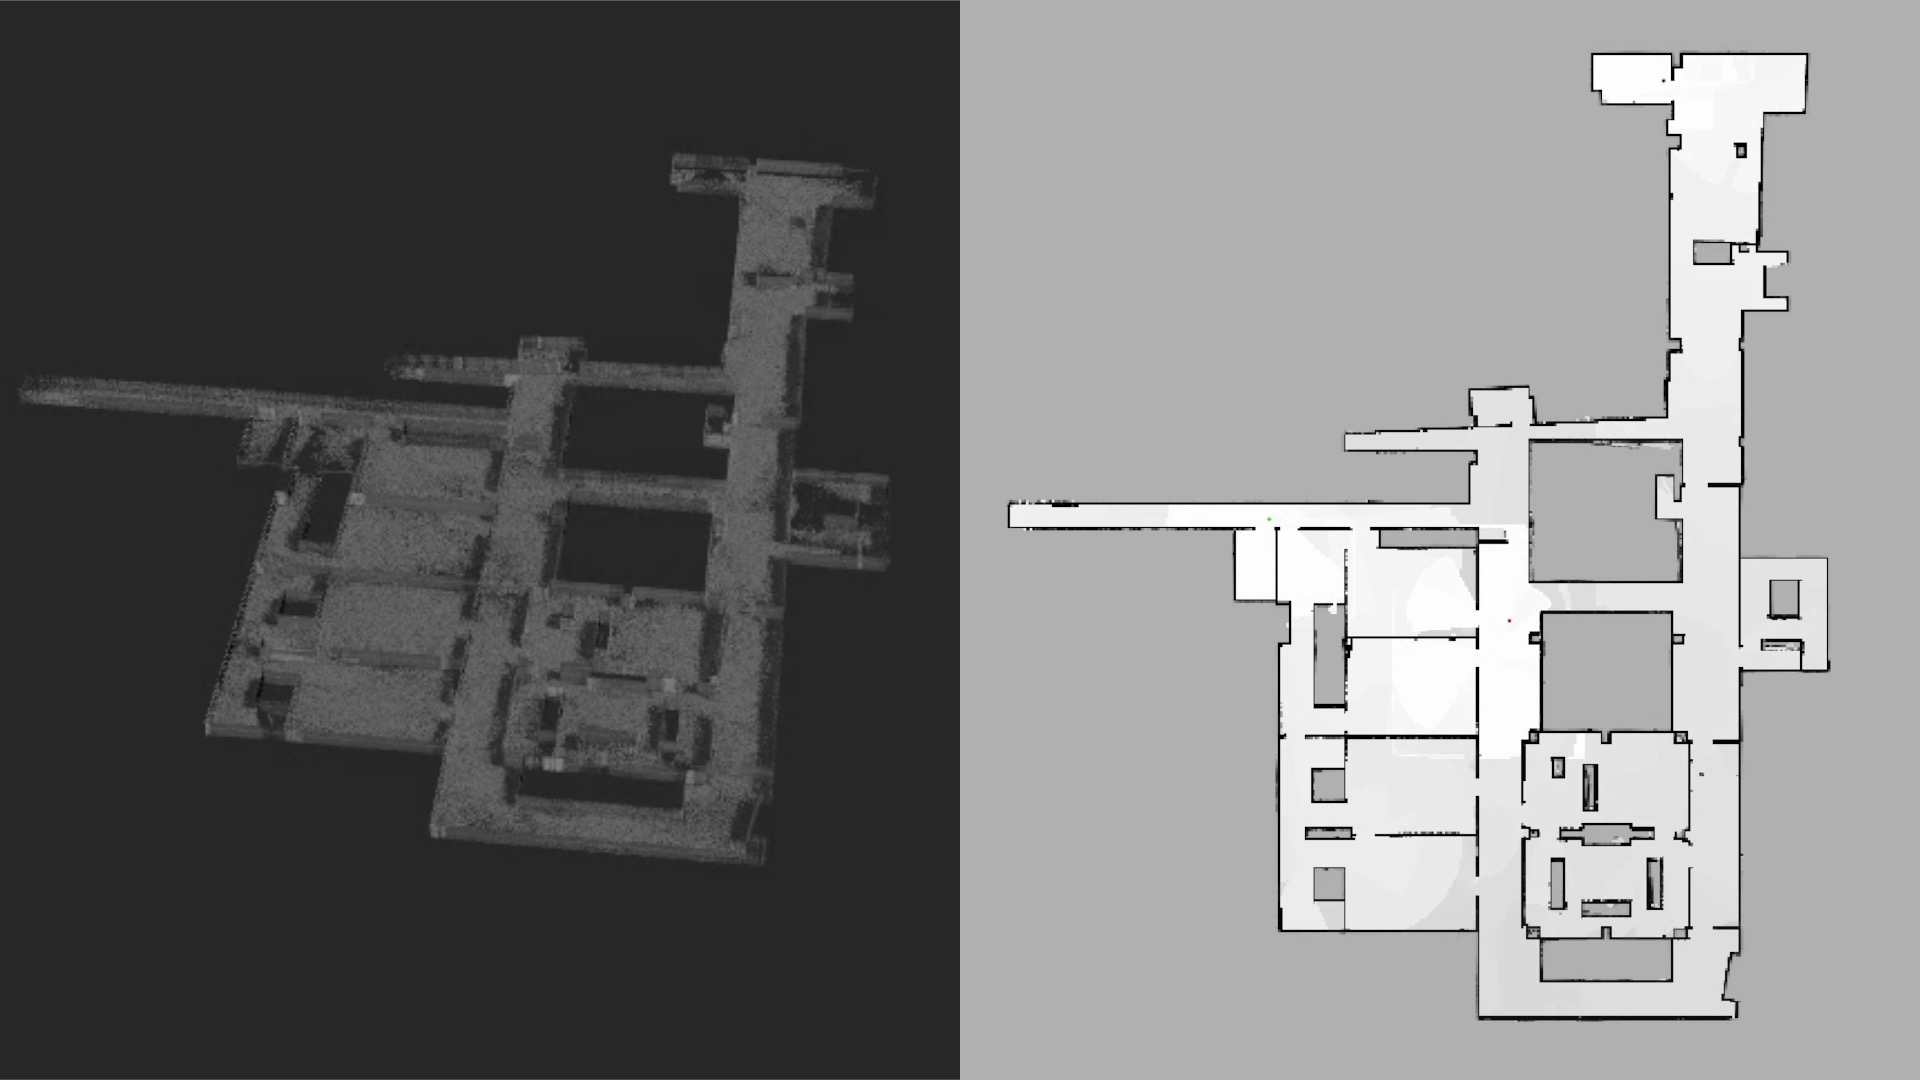
\includegraphics[trim={0cm 0cm 35cm 0cm}, clip, width=\textwidth]{Patrol_Split_Screen_9min.jpg}
        		\caption{$9$ min}
		\vspace*{0.05\textwidth}
    	\end{subfigure}
	\hspace*{0.05\textwidth}
    	\begin{subfigure}[t]{0.38\columnwidth}
           	\centering
          	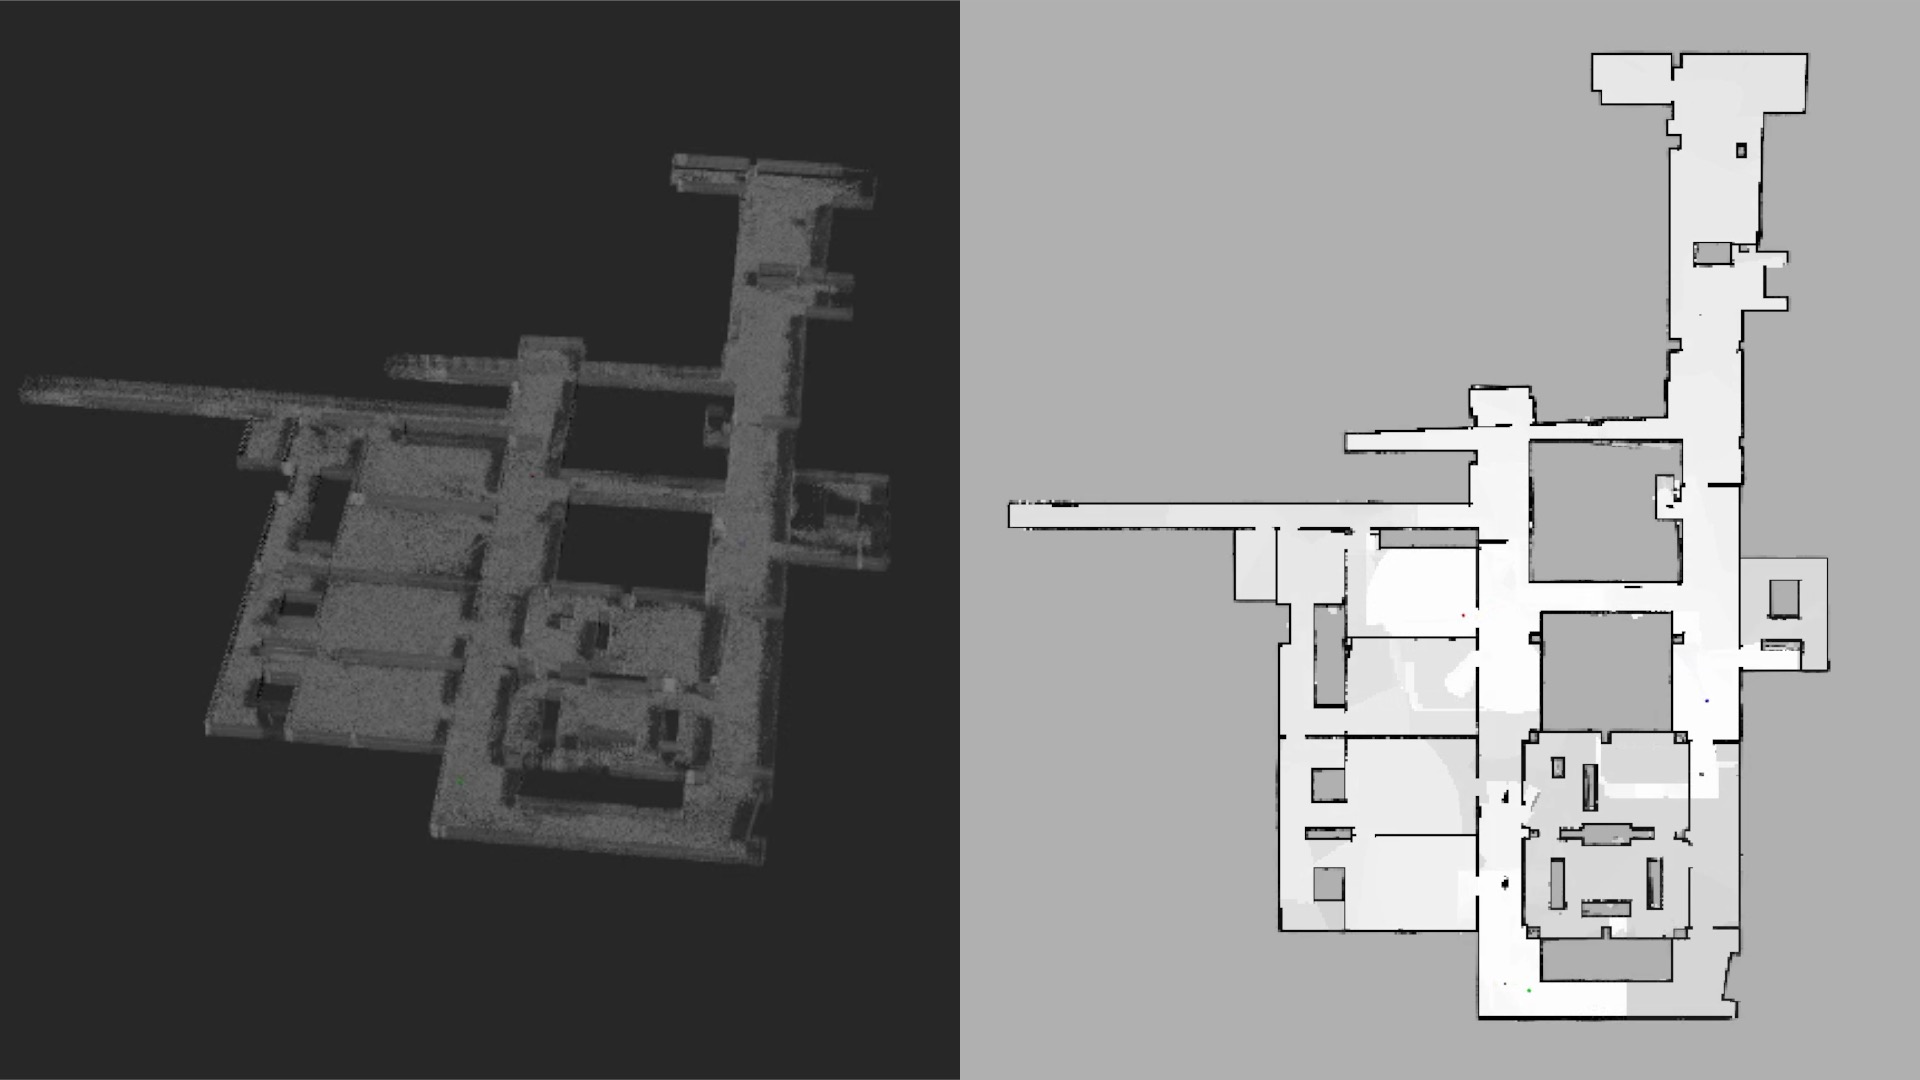
\includegraphics[trim={0cm 0cm 35cm 0cm}, clip, width=\textwidth]{Patrol_Split_Screen_11min.jpg}
        		\caption{$11$ min}
		\vspace*{0.05\textwidth}
    	\end{subfigure}
    	\begin{subfigure}[t]{0.38\columnwidth}
           	\centering
          	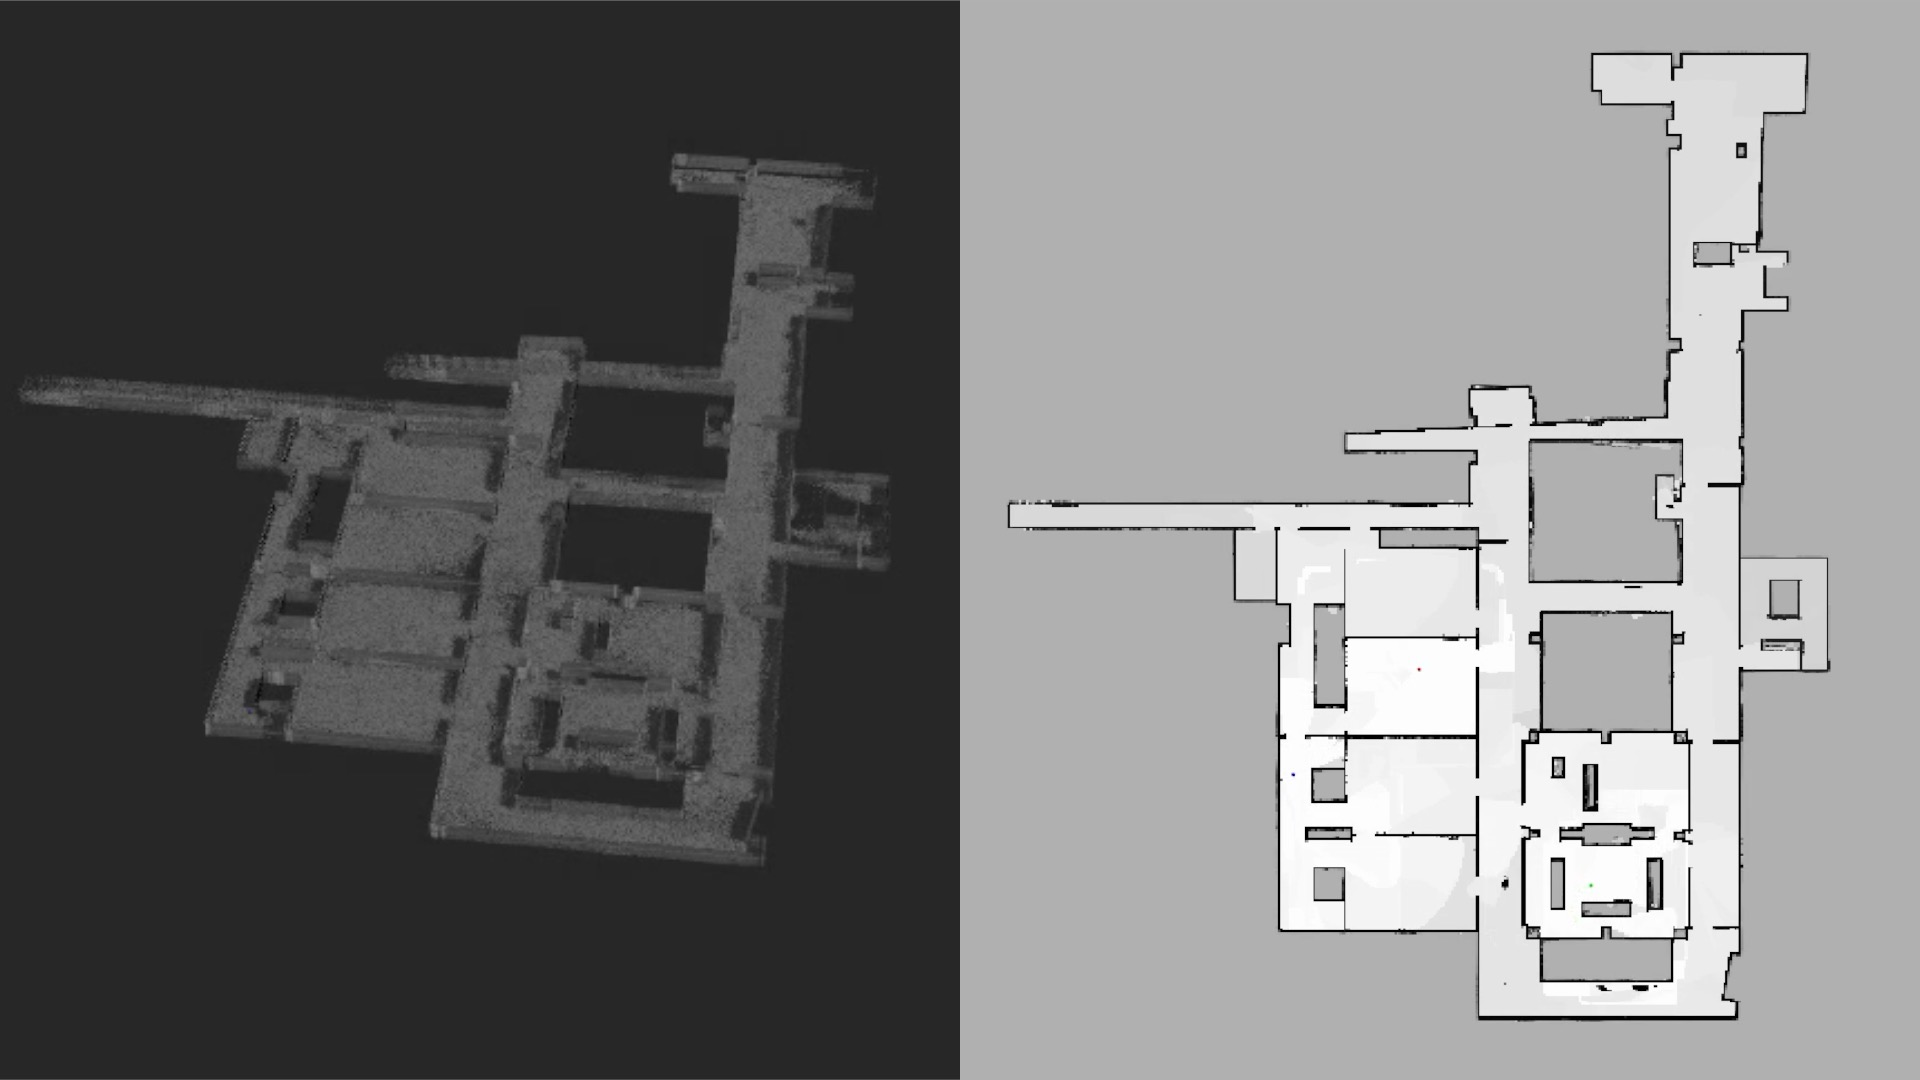
\includegraphics[trim={0cm 0cm 35cm 0cm}, clip, width=\textwidth]{Patrol_Split_Screen_13min.jpg}
        		\caption{$13$ min}
		\vspace*{0.05\textwidth}
    	\end{subfigure}
	\hspace*{0.05\textwidth}
    	\begin{subfigure}[t]{0.38\columnwidth}
           	\centering
          	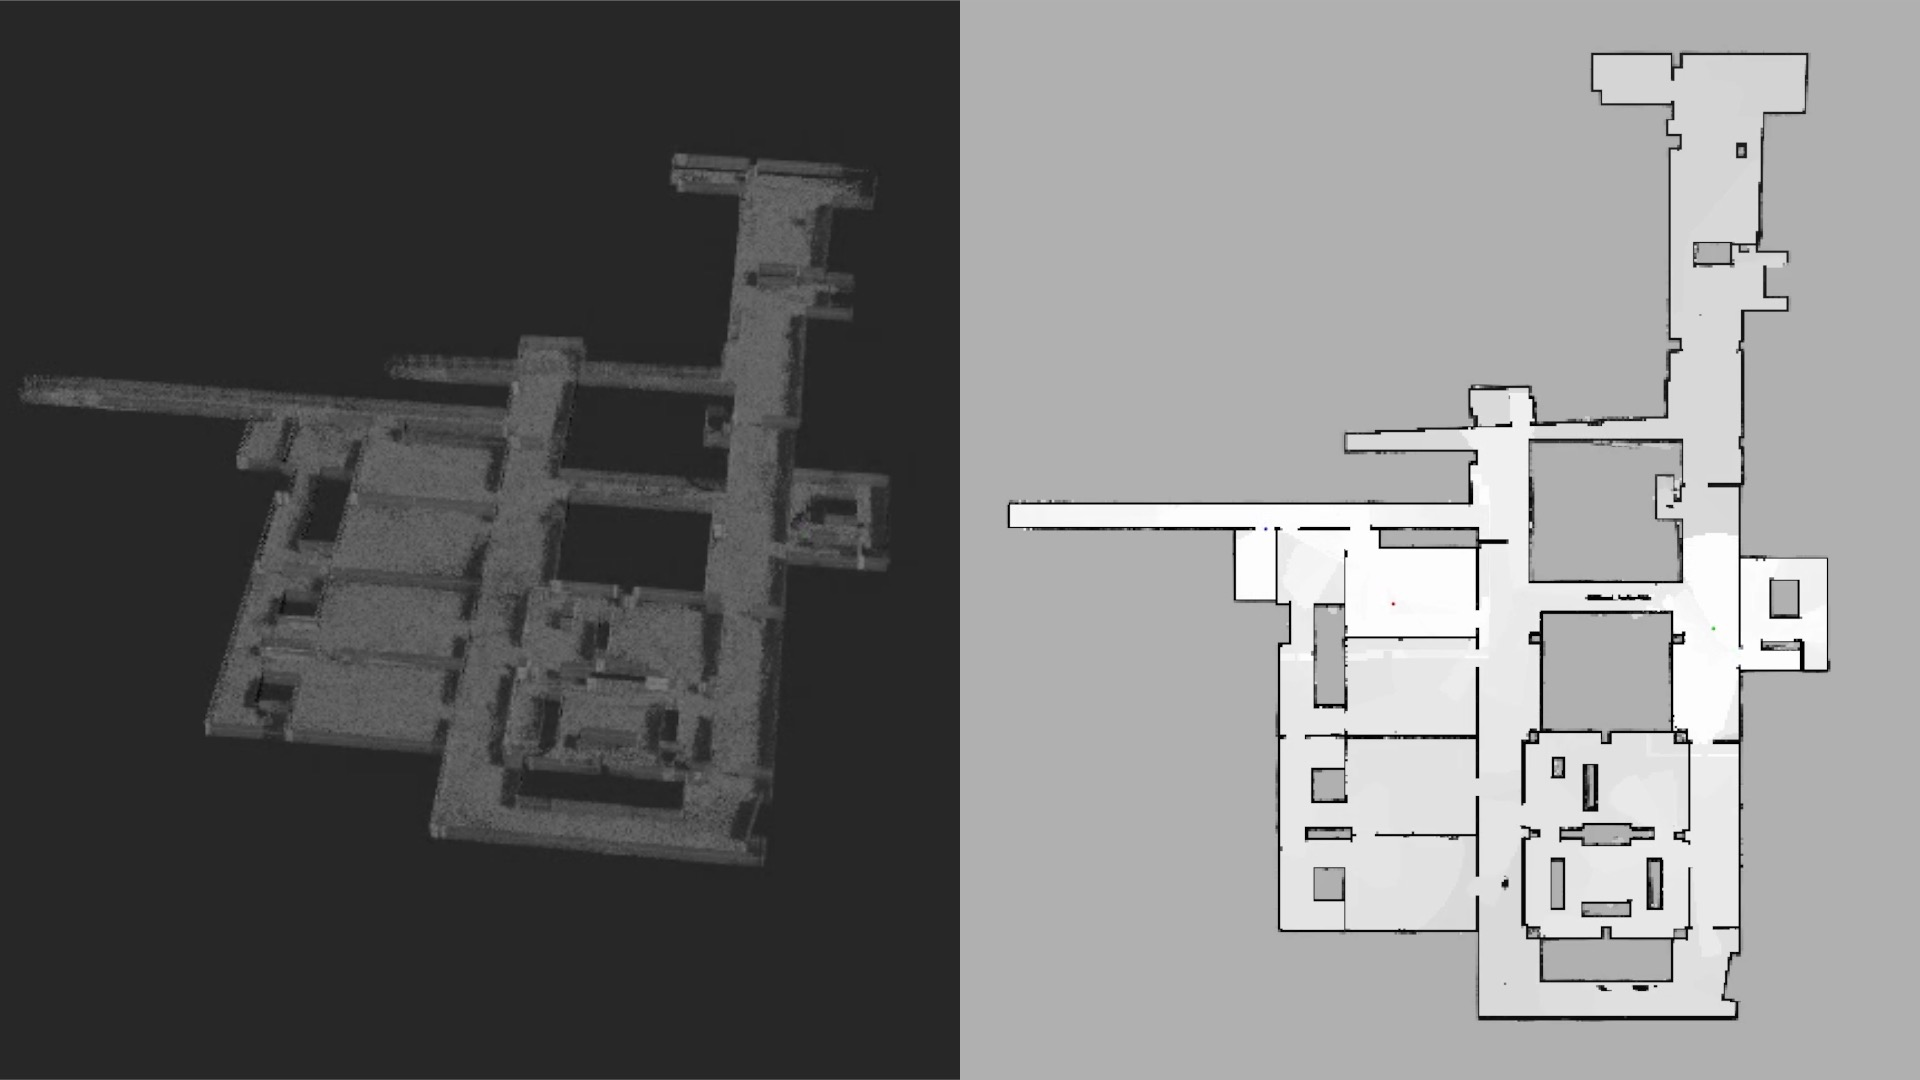
\includegraphics[trim={0cm 0cm 35cm 0cm}, clip, width=\textwidth]{Patrol_Split_Screen_15min.jpg}
        		\caption{$15$ min}
		\vspace*{0.05\textwidth}
    	\end{subfigure}
	\caption{The 3D occupancy grid map representation of the SEH second floor is shown during patrol. The robots generate these maps while avoiding collisions with each other, the environment, and a non-cooperative human.}
	\label{fig:sim3DMap}
\end{figure}

\begin{figure}[!t]
\centering
    	\begin{subfigure}[t]{0.38\columnwidth}
           	\centering
          	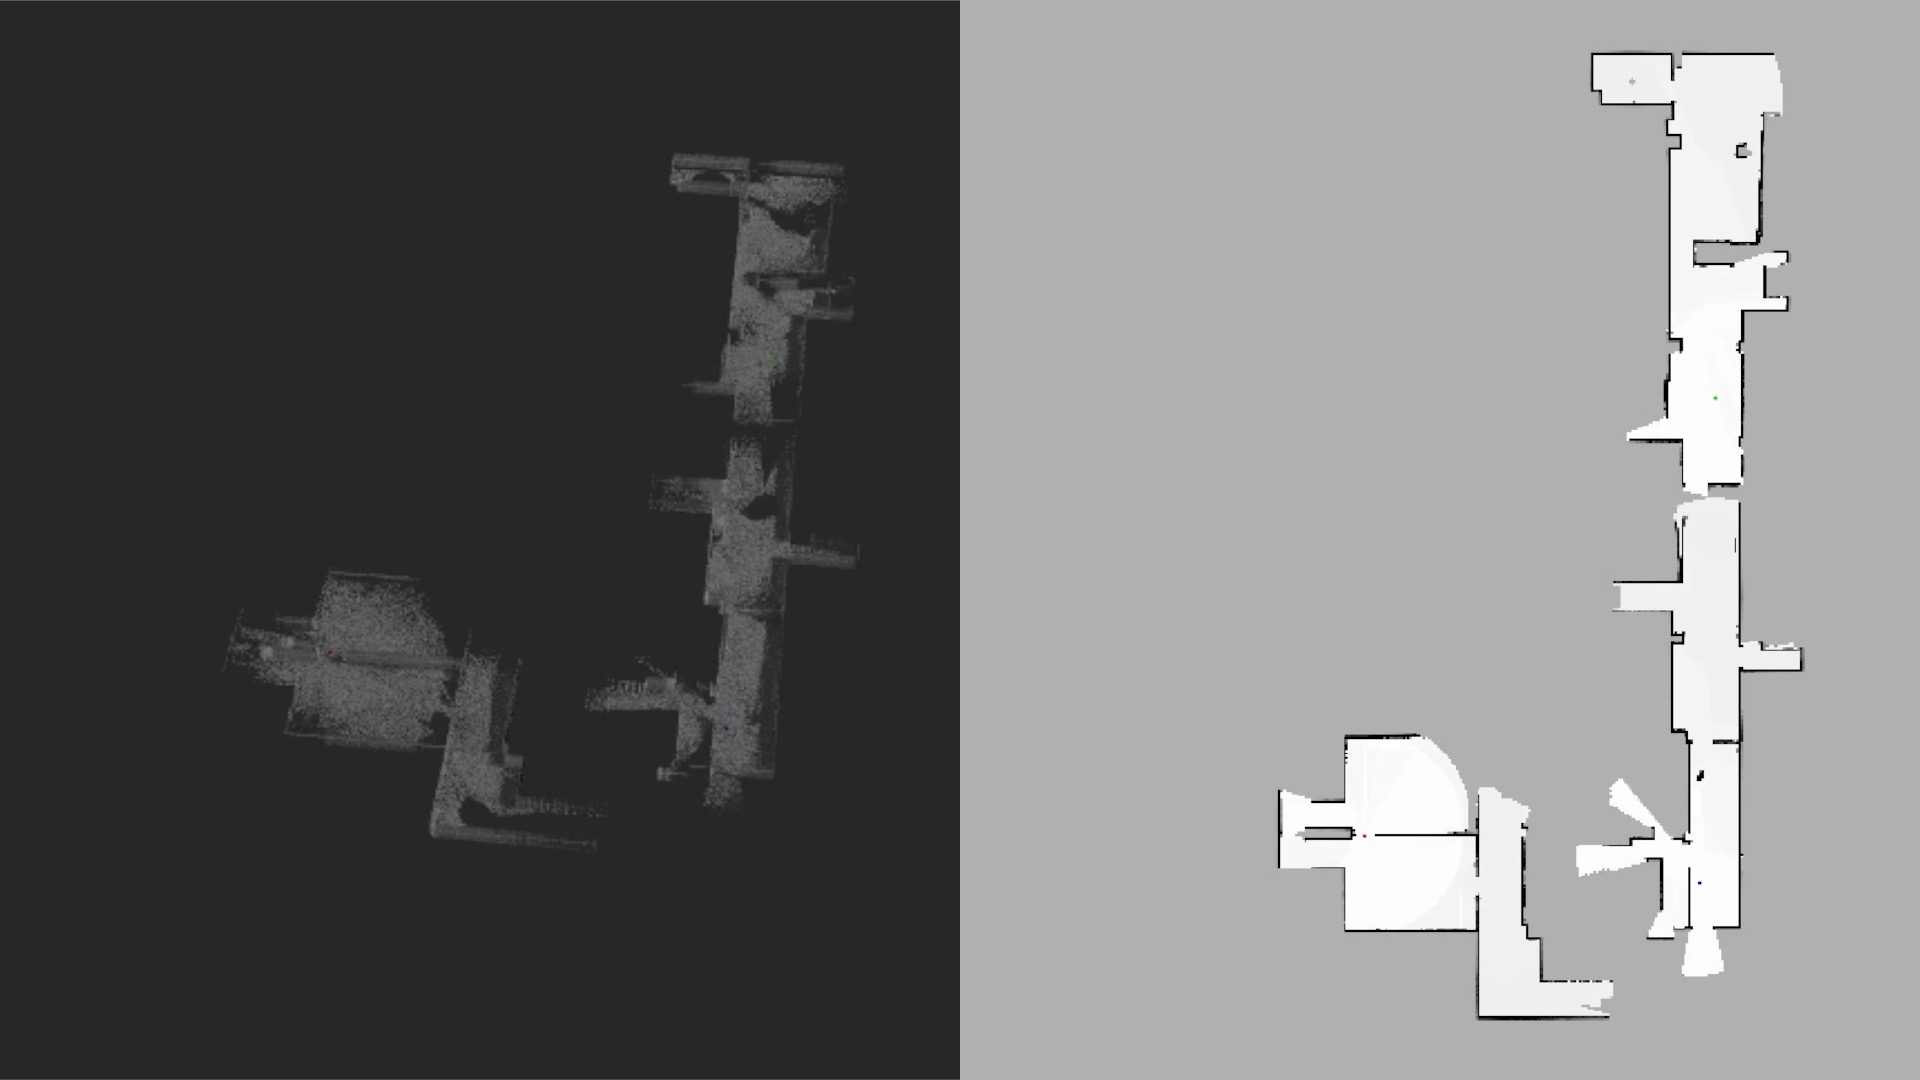
\includegraphics[trim={35cm 0cm 0cm 0cm}, clip, width=\textwidth]{Patrol_Split_Screen_1min.jpg}
        		\caption{$1$ min}
		\vspace*{0.05\textwidth}
    	\end{subfigure}
	\hspace*{0.05\textwidth}
    	\begin{subfigure}[t]{0.38\columnwidth}
           	\centering
          	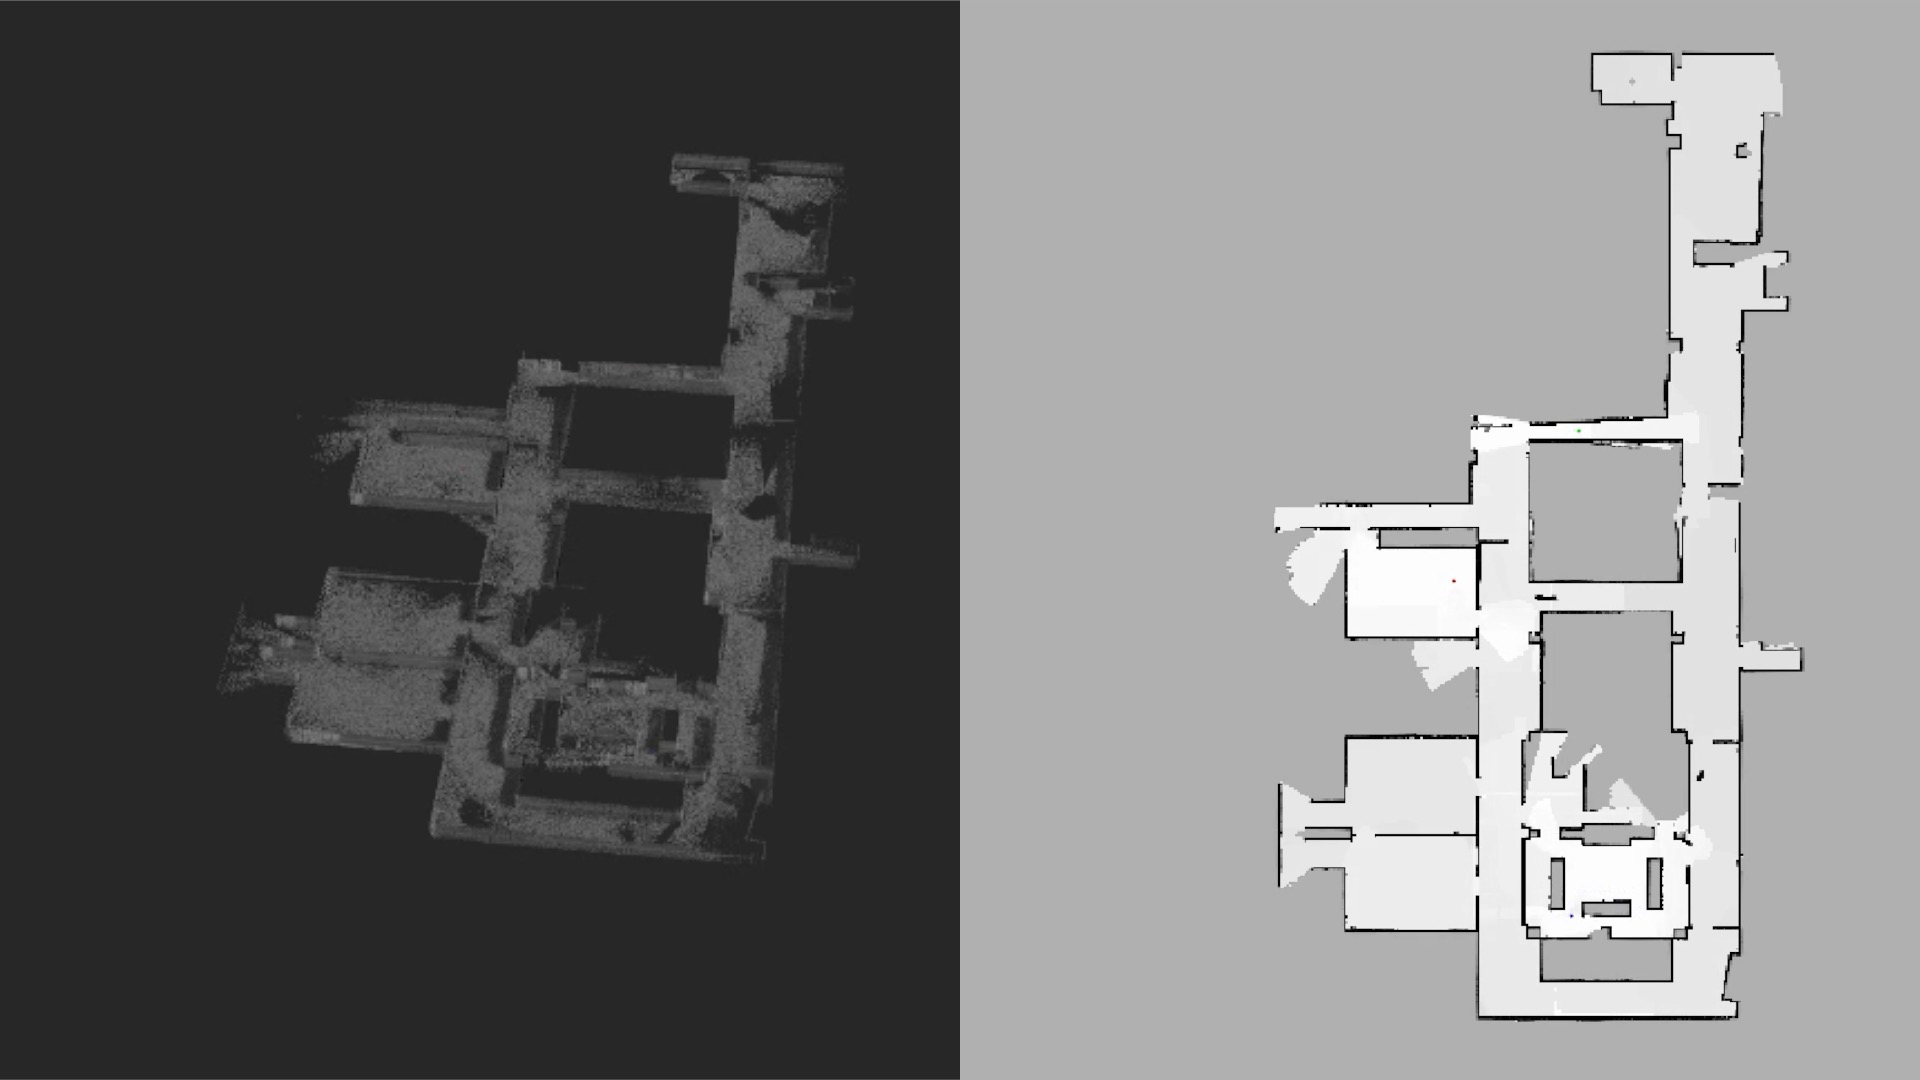
\includegraphics[trim={35cm 0cm 0cm 0cm}, clip, width=\textwidth]{Patrol_Split_Screen_3min.jpg}
        		\caption{$3$ min}
		\vspace*{0.05\textwidth}
    	\end{subfigure}
	\begin{subfigure}[t]{0.38\columnwidth}
           	\centering
          	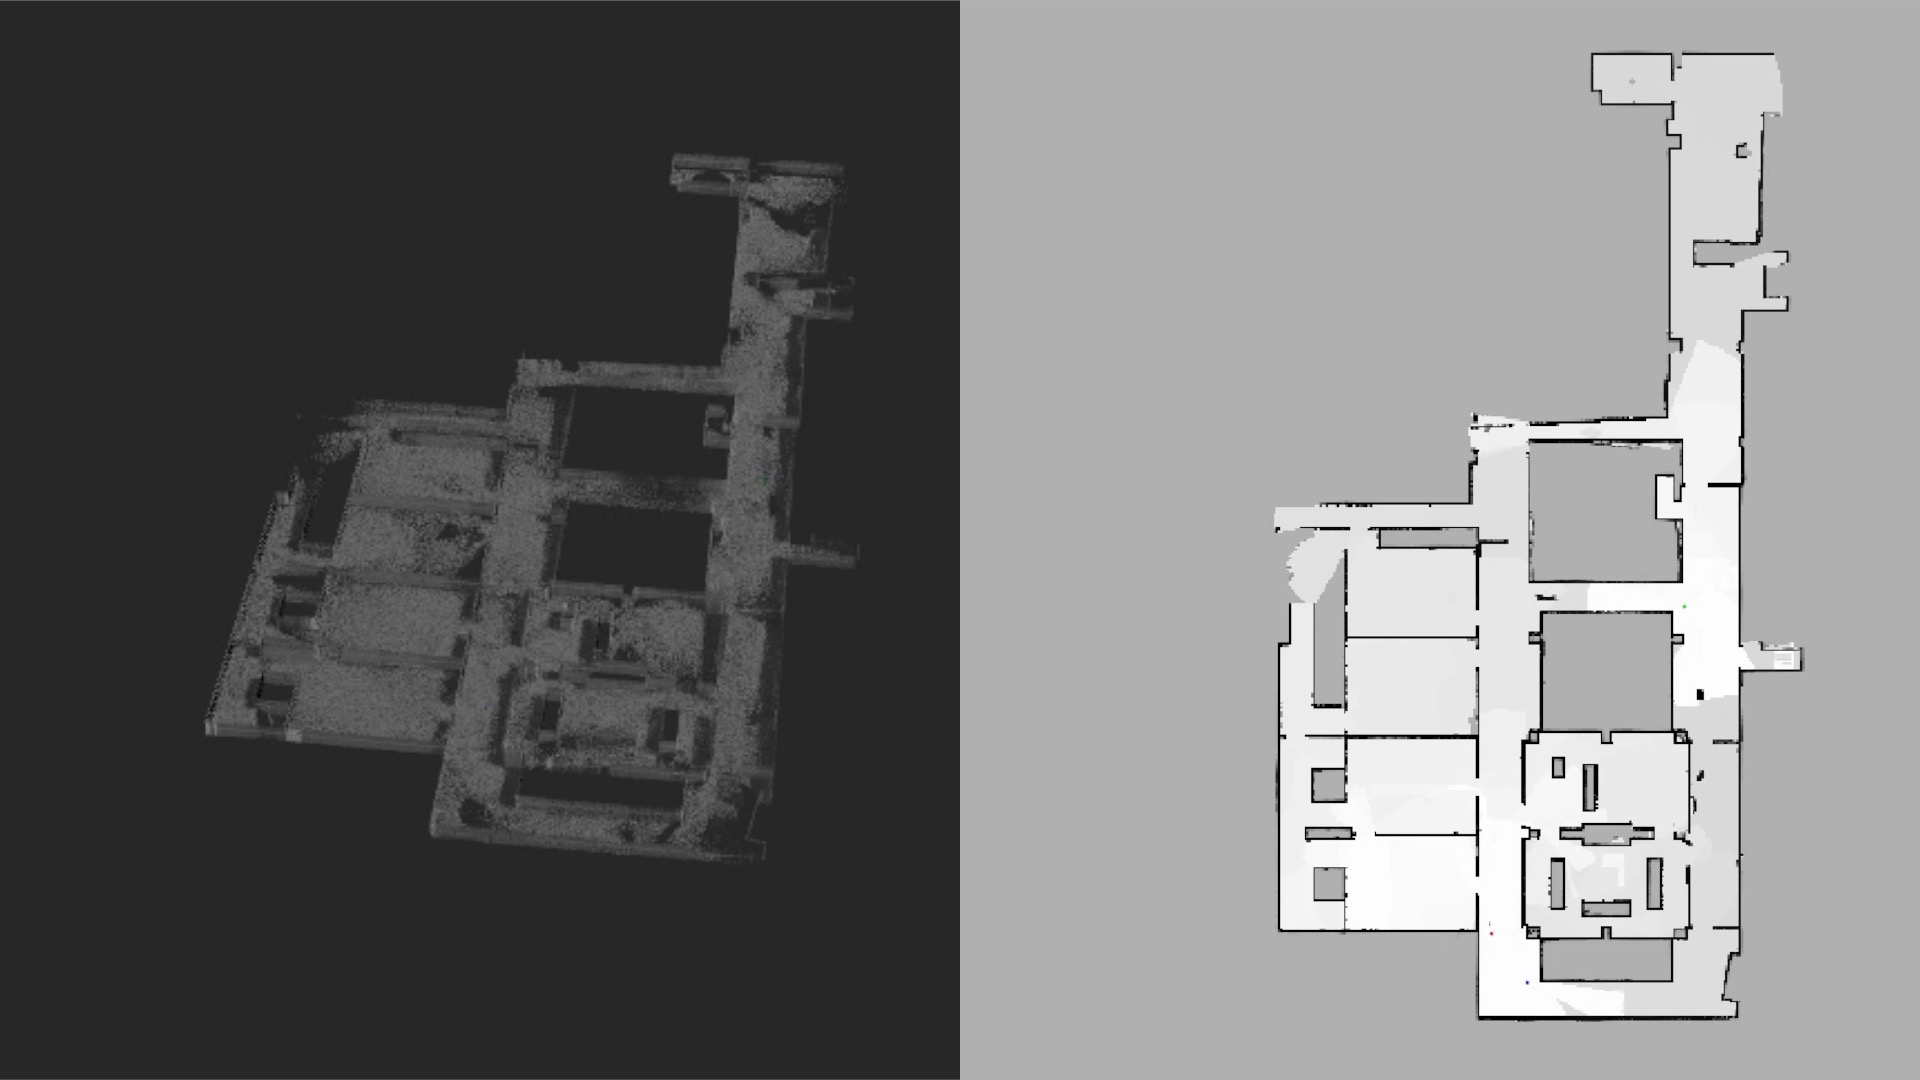
\includegraphics[trim={35cm 0cm 0cm 0cm}, clip, width=\textwidth]{Patrol_Split_Screen_5min.jpg}
        		\caption{$5$ min}
		\vspace*{0.05\textwidth}
    	\end{subfigure}
	\hspace*{0.05\textwidth}
    	\begin{subfigure}[t]{0.38\columnwidth}
           	\centering
          	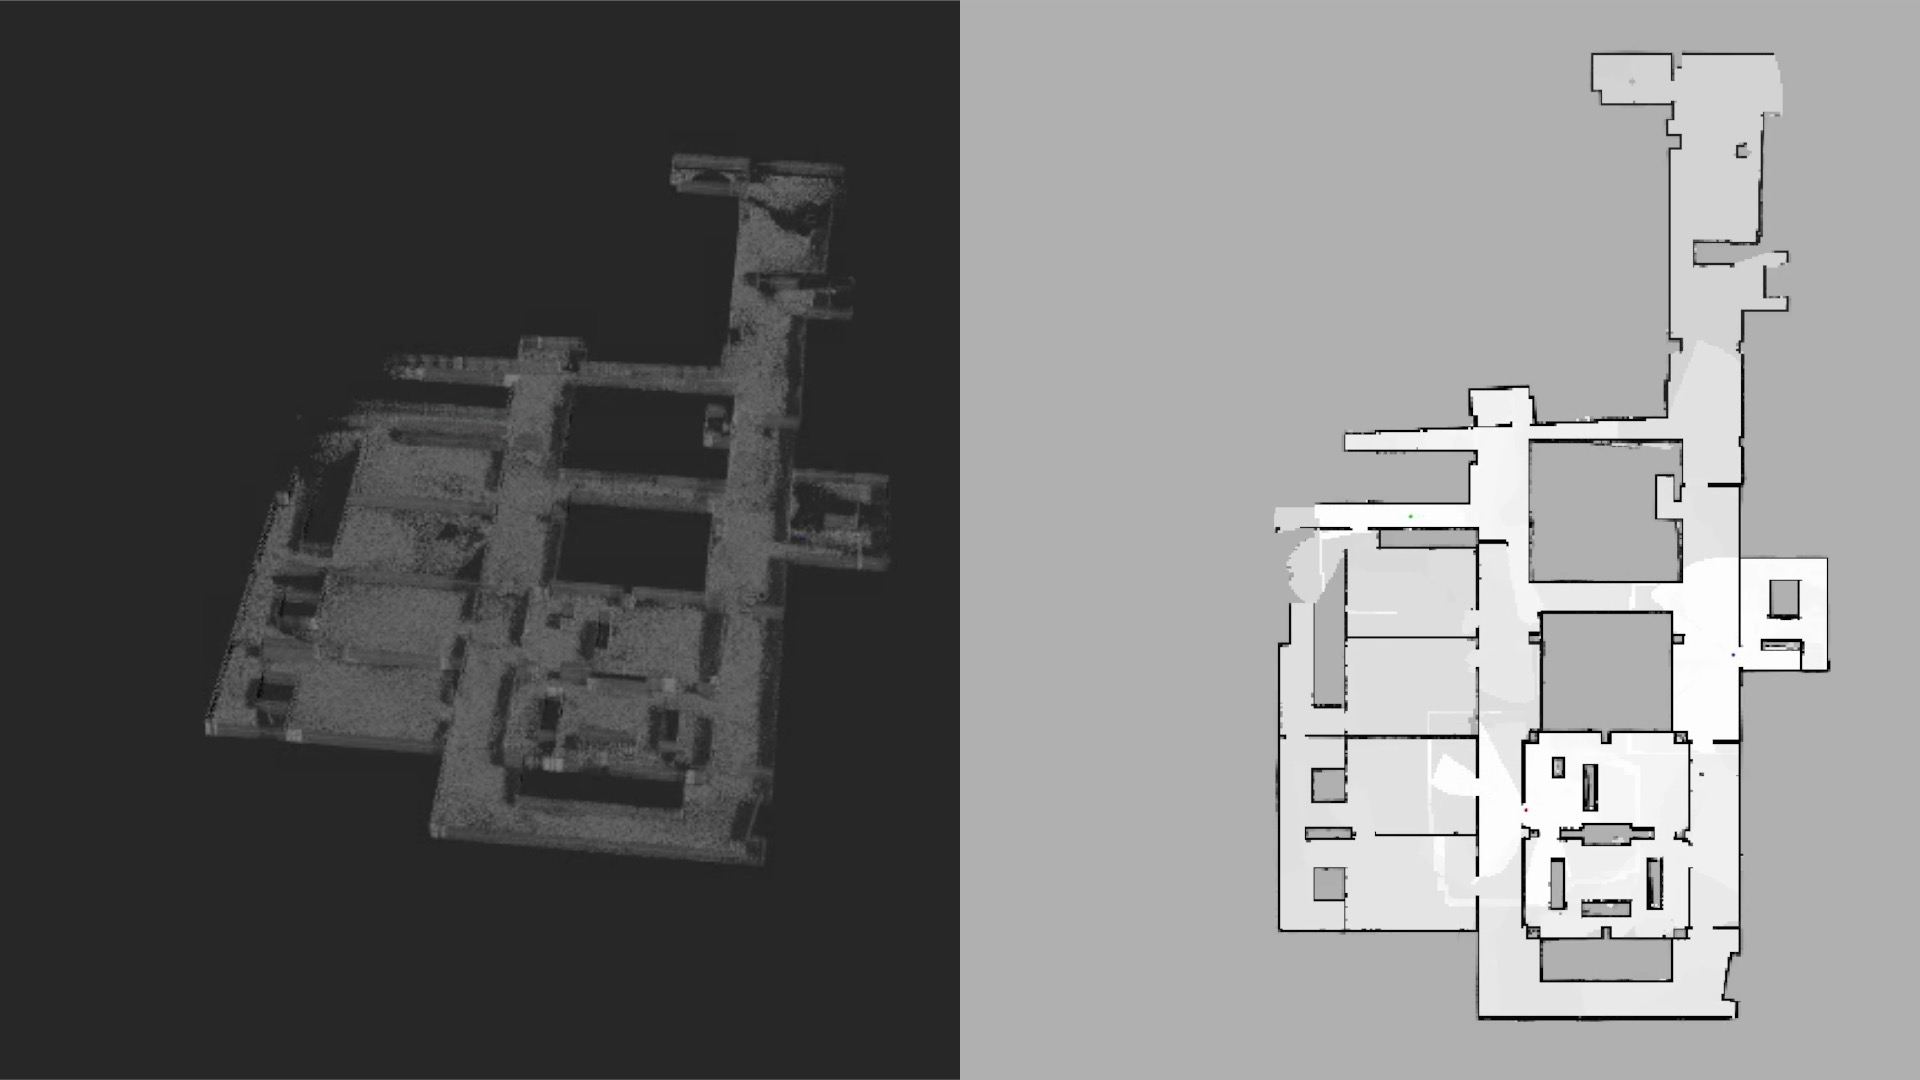
\includegraphics[trim={35cm 0cm 0cm 0cm}, clip, width=\textwidth]{Patrol_Split_Screen_7min.jpg}
        		\caption{$7$ min}
		\vspace*{0.05\textwidth}
    	\end{subfigure}
    	\begin{subfigure}[t]{0.38\columnwidth}
           	\centering
          	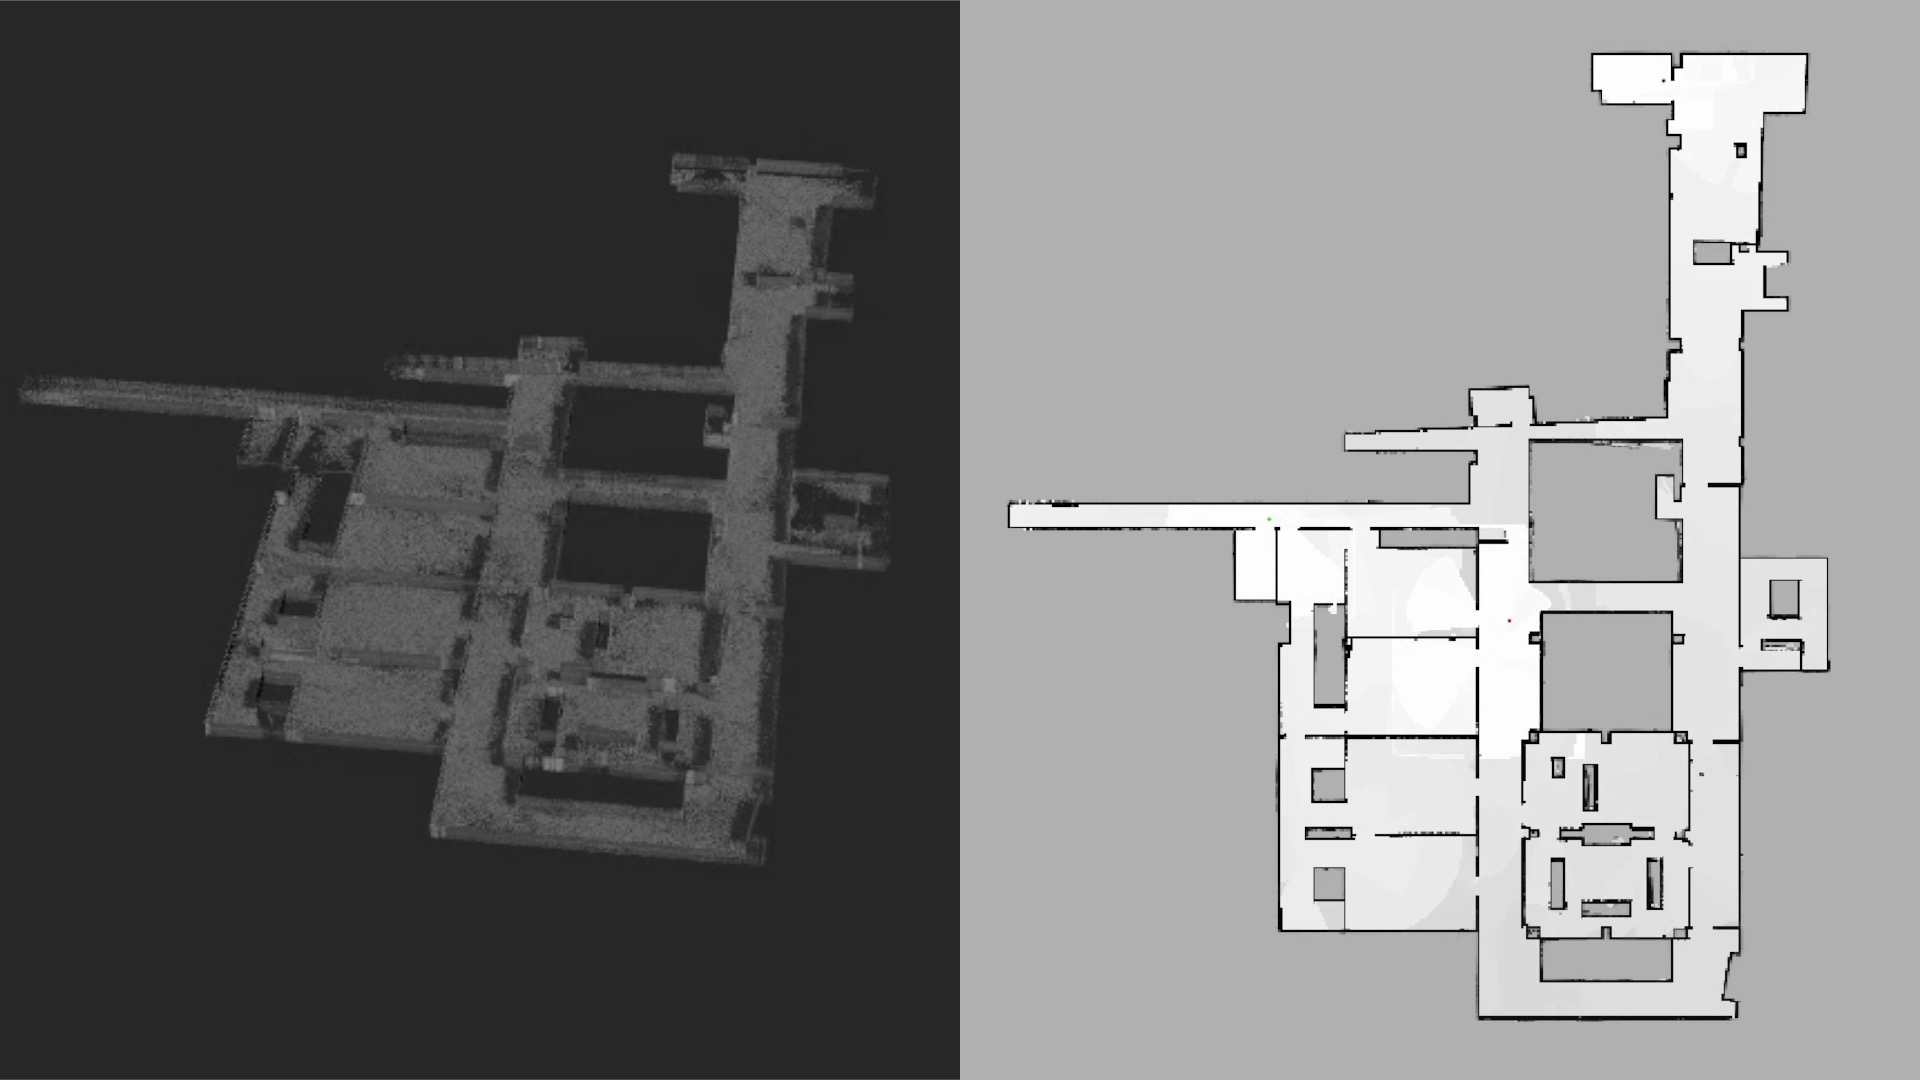
\includegraphics[trim={35cm 0cm 0cm 0cm}, clip, width=\textwidth]{Patrol_Split_Screen_9min.jpg}
        		\caption{$9$ min}
		\vspace*{0.05\textwidth}
    	\end{subfigure}
	\hspace*{0.05\textwidth}
    	\begin{subfigure}[t]{0.38\columnwidth}
           	\centering
          	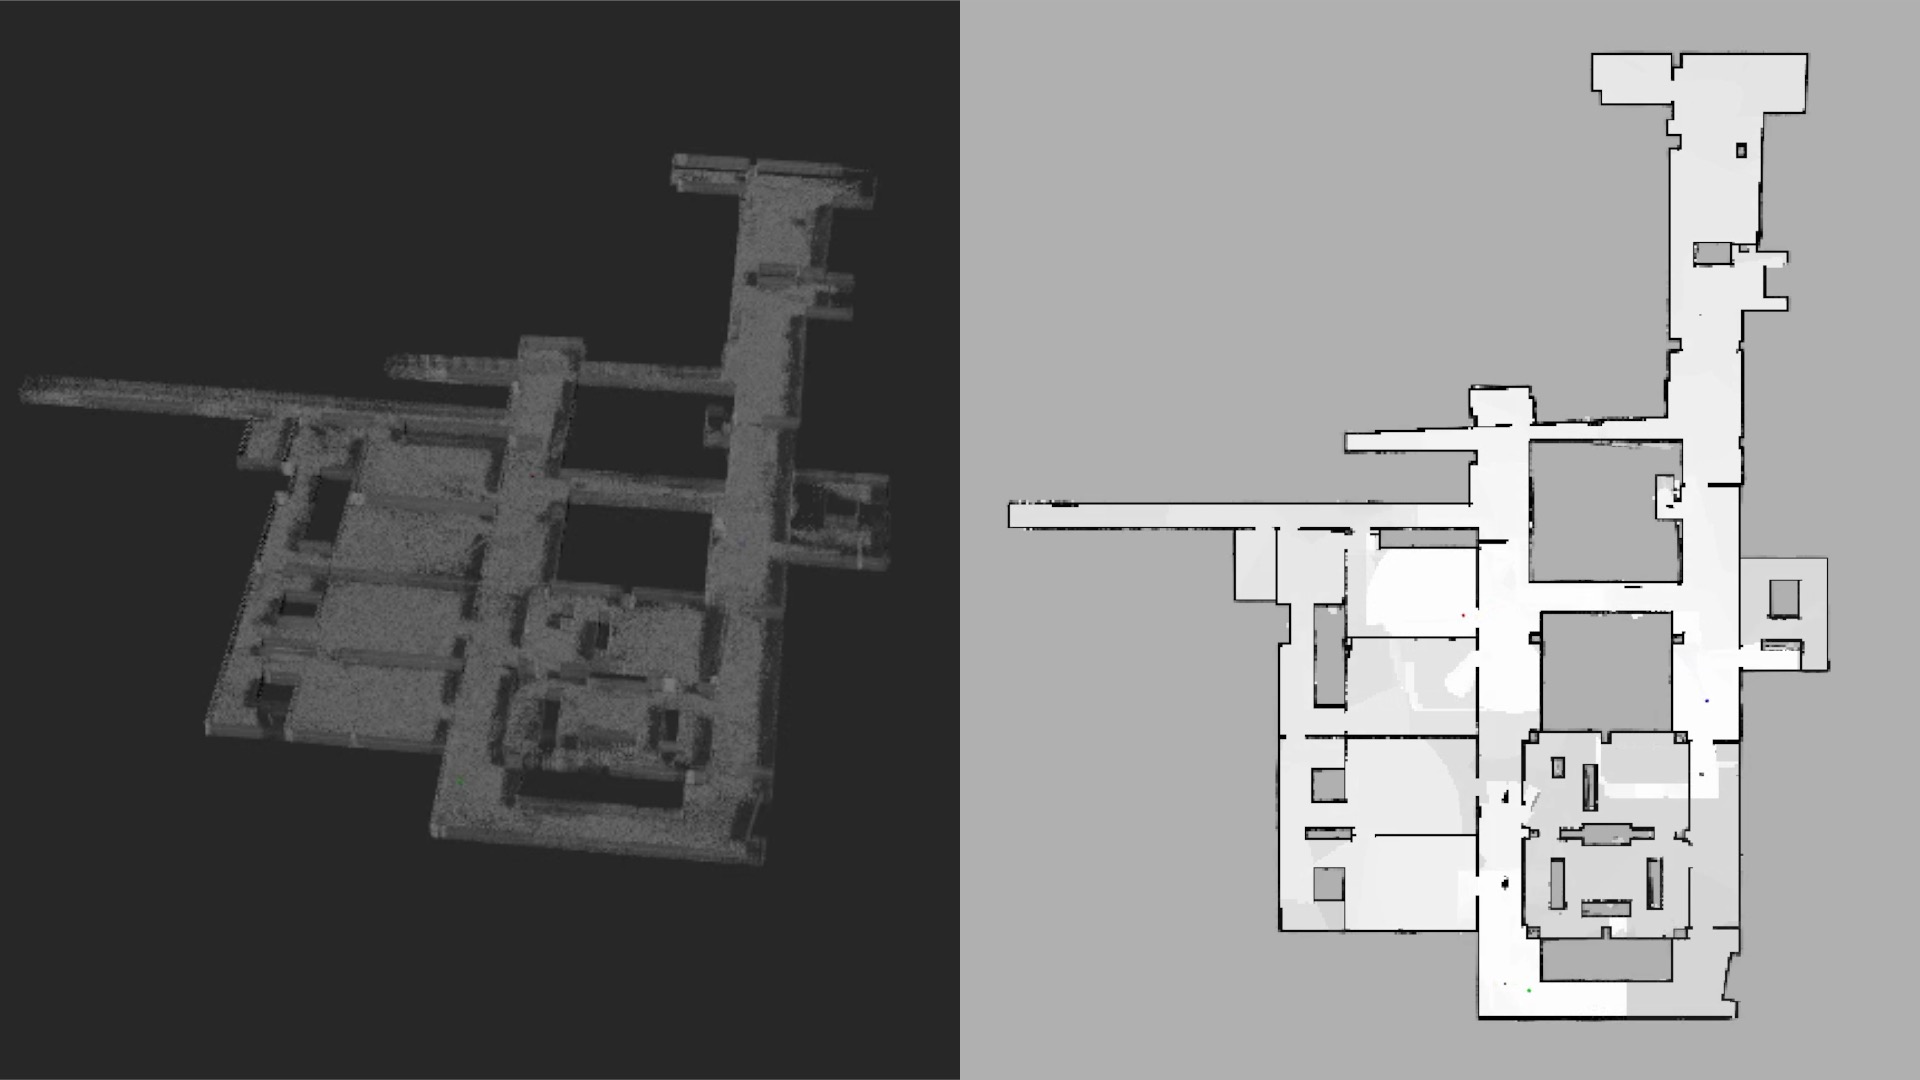
\includegraphics[trim={35cm 0cm 0cm 0cm}, clip, width=\textwidth]{Patrol_Split_Screen_11min.jpg}
        		\caption{$11$ min}
		\vspace*{0.05\textwidth}
    	\end{subfigure}
    	\begin{subfigure}[t]{0.38\columnwidth}
           	\centering
          	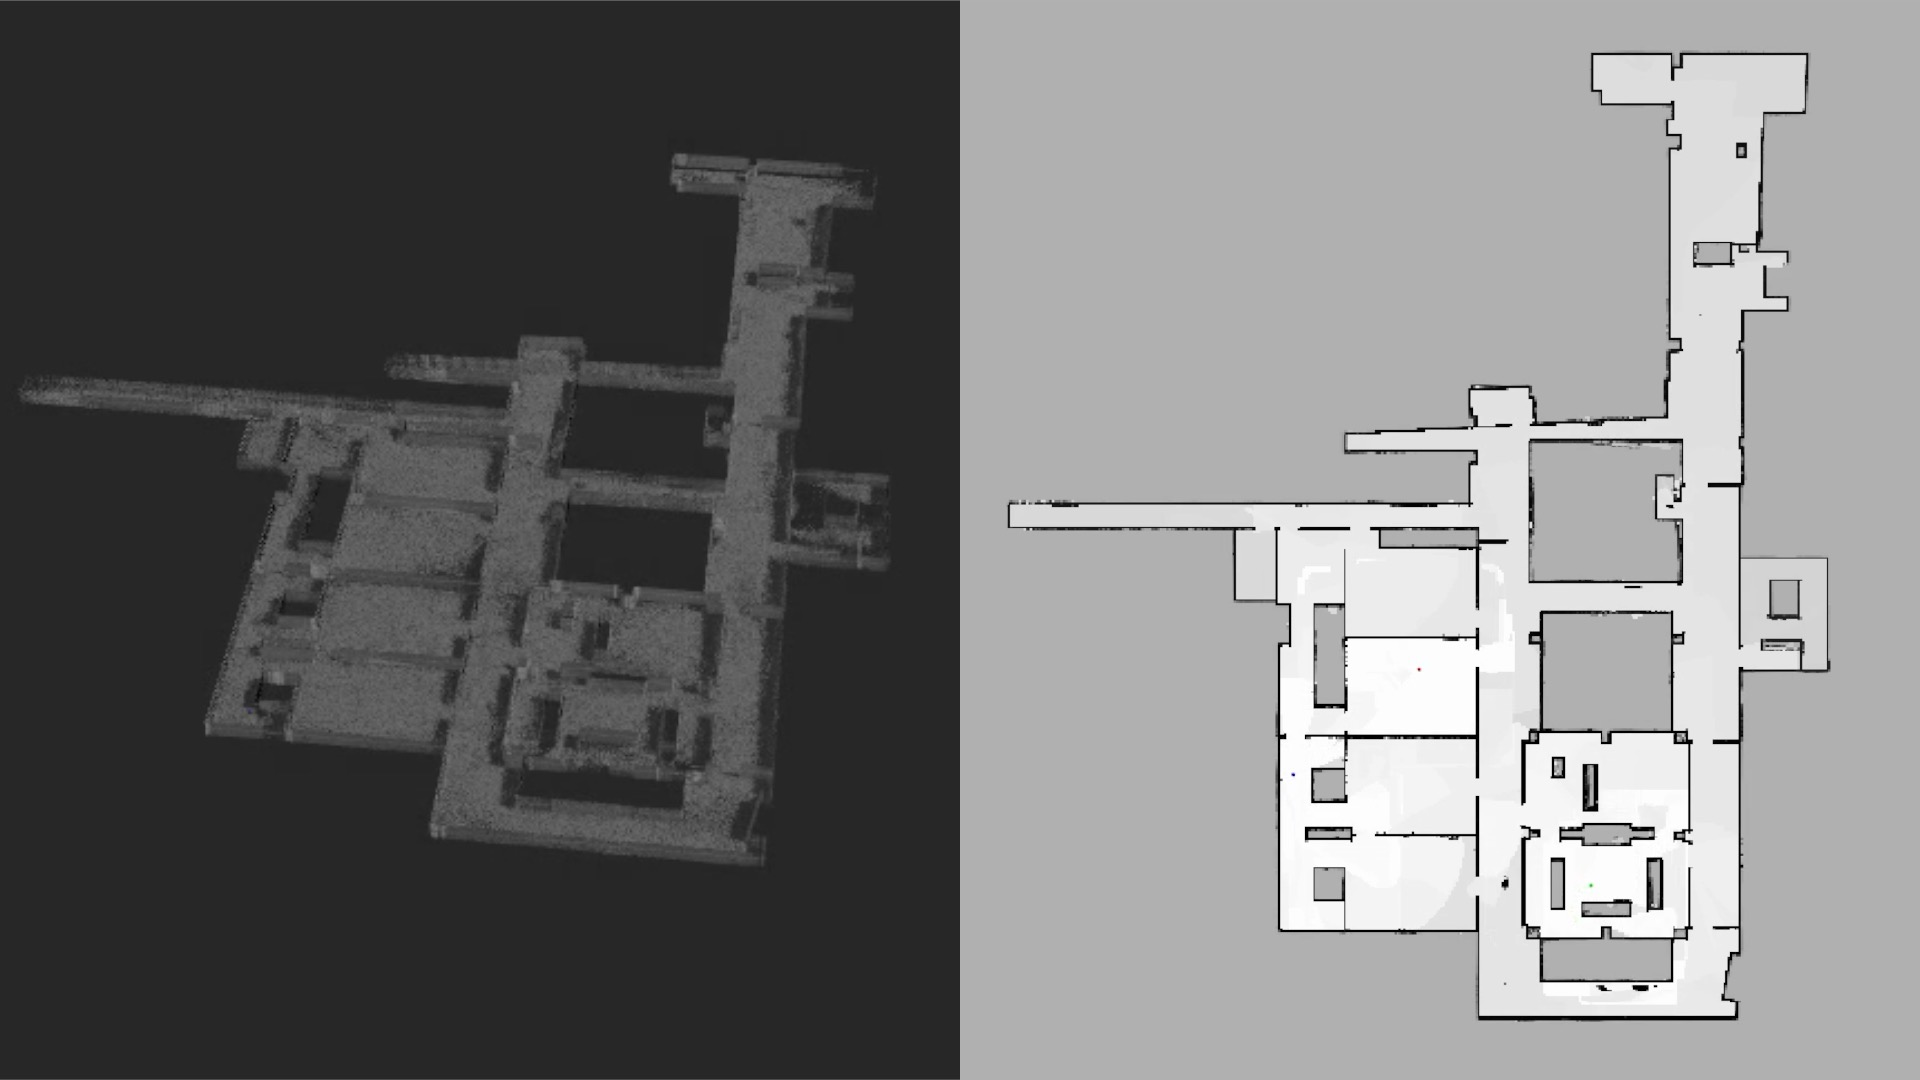
\includegraphics[trim={35cm 0cm 0cm 0cm}, clip, width=\textwidth]{Patrol_Split_Screen_13min.jpg}
        		\caption{$13$ min}
		\vspace*{0.05\textwidth}
    	\end{subfigure}
	\hspace*{0.05\textwidth}
    	\begin{subfigure}[t]{0.38\columnwidth}
           	\centering
          	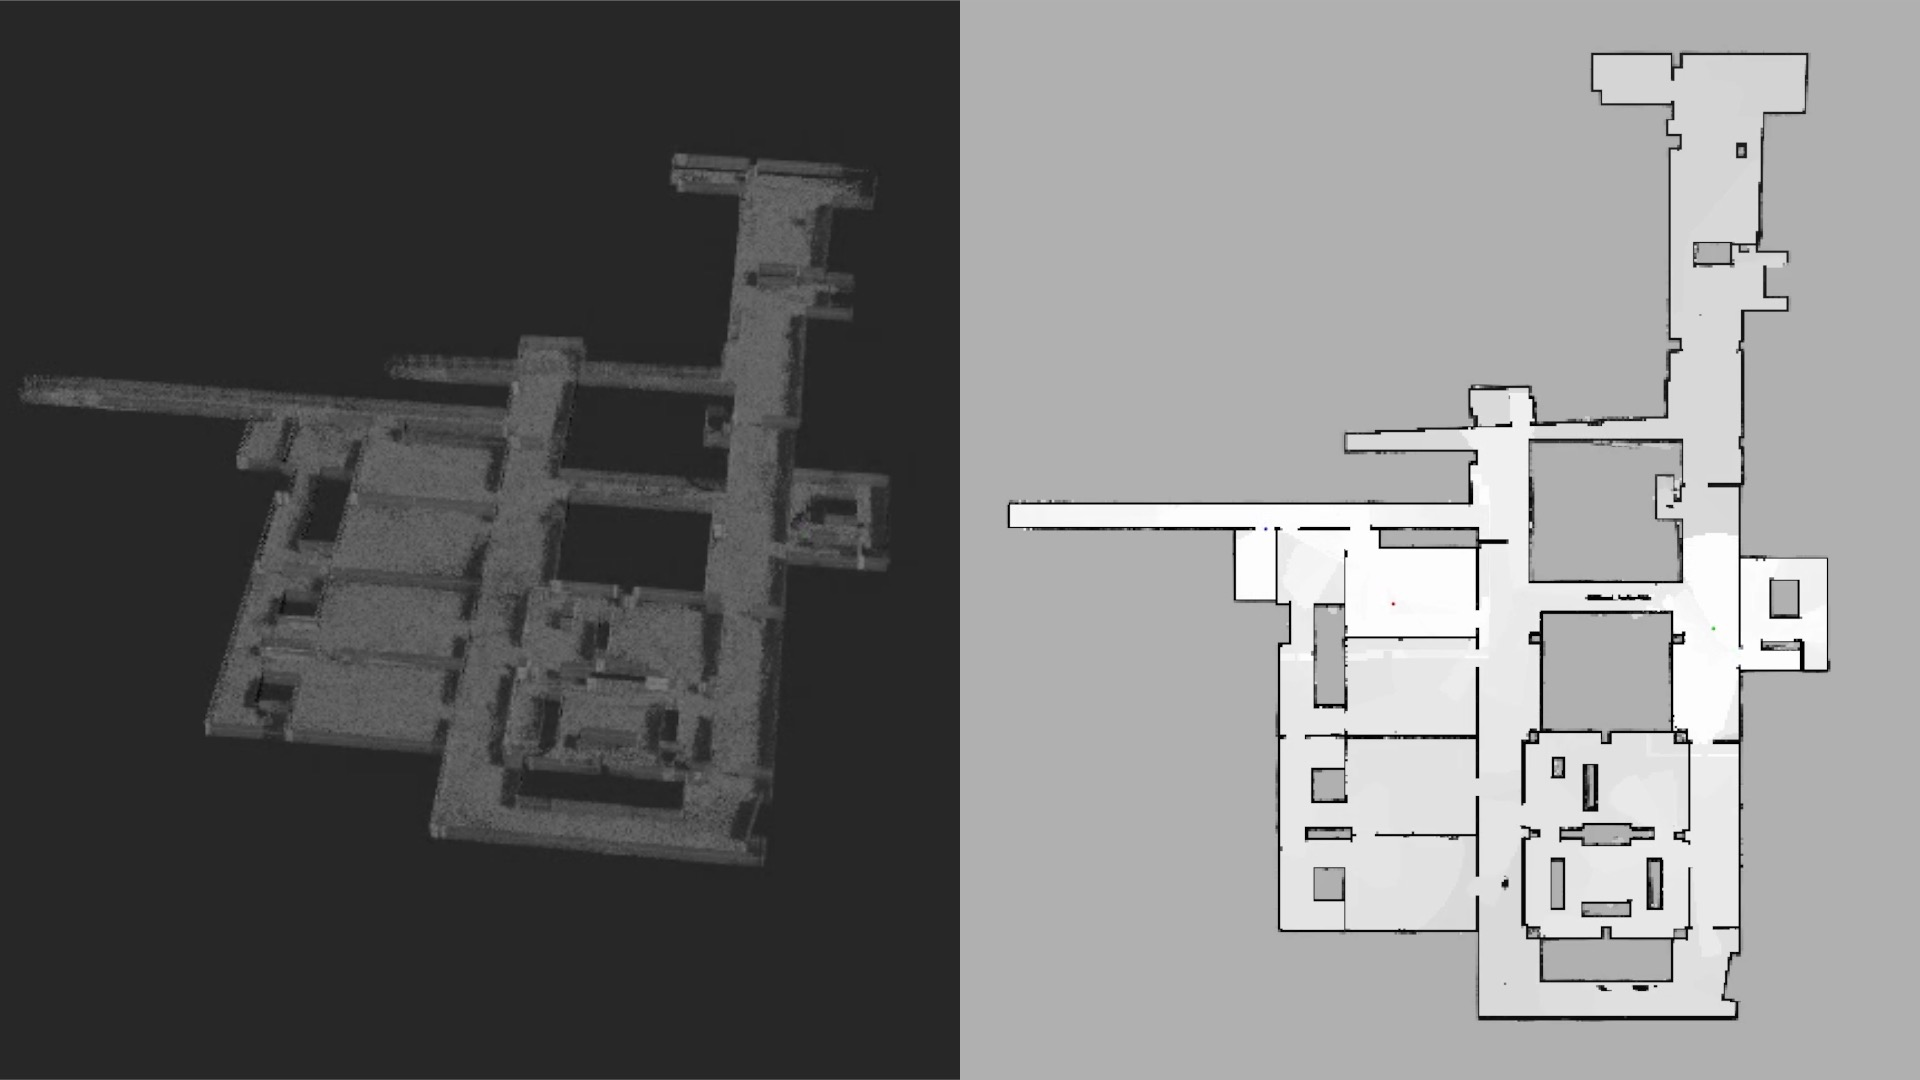
\includegraphics[trim={35cm 0cm 0cm 0cm}, clip, width=\textwidth]{Patrol_Split_Screen_15min.jpg}
        		\caption{$15$ min}
		\vspace*{0.05\textwidth}
    	\end{subfigure}
	\caption{The 2D projected map from of the SEH second floor shows degradation while robots patrol the space. The robots evade the non-cooperative human walking in a rectangular pattern, occasionally capturing the temporarily-occupied space and identifying these cells as occupied on the grid.}
	\label{fig:sim2Dmaps}
\end{figure}
%	% trim={<left> <lower> <right> <upper>}


The robot generated a fairly-complete occupancy grid within $9$ minutes, and proceeded to patrol the space during the remaining time. After $9$ minutes, the total map entropy no longer increases or decreases significantly; the rate at which cell degradation increases map entropy roughly cancels the rate at which new measurements decrease map entropy. In contrast, if the robots simply hover instead of patrol after $9$ minutes, the map uncertainty quickly increases, shown in Fig. \ref{fig:DegradeExamples}.

\begin{figure}
\centering
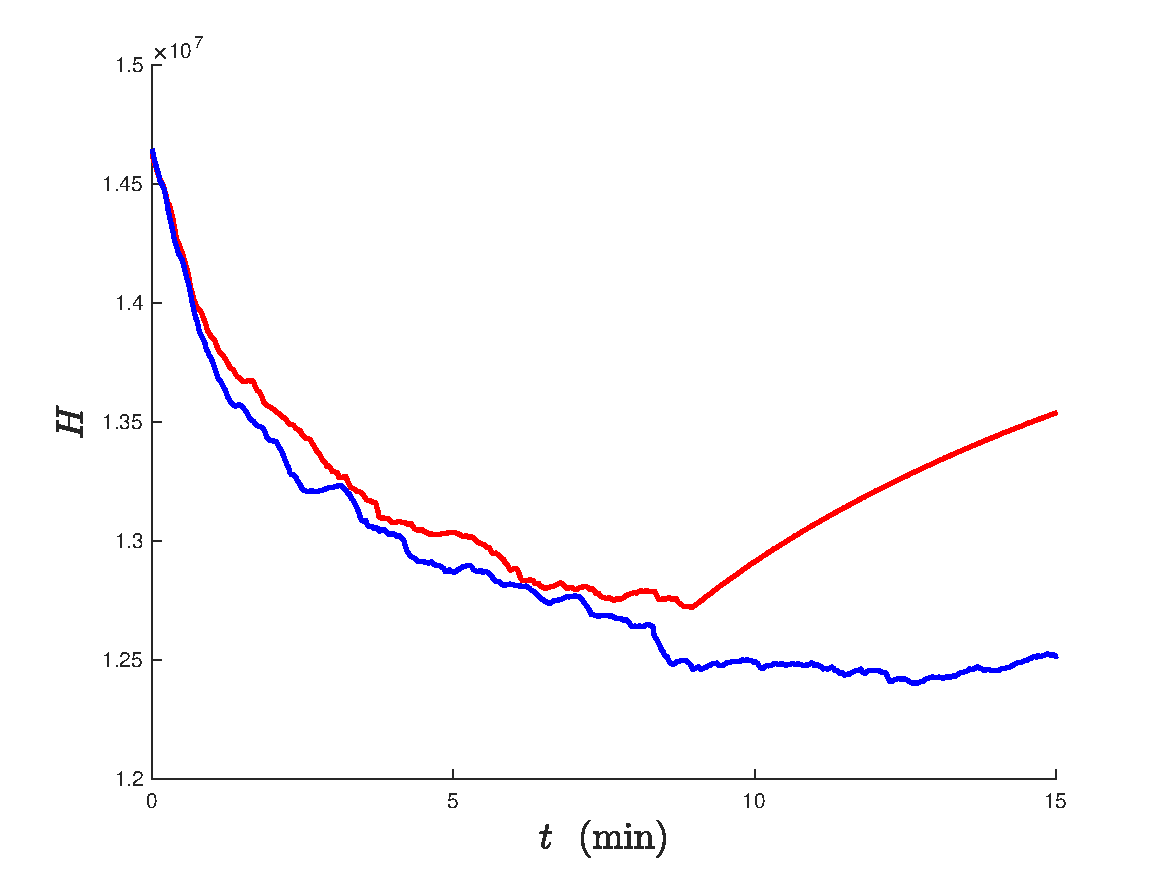
\includegraphics[width=\textwidth]{entropy_patrol_9minSwitch.pdf}
\caption{Total map entropies are tracked for separate trials: patrol of the building for $15$ minutes (blue) and patrol of the building for $9$ minutes, then hover (red). Even though the map is fairly well-known after $9$ minutes in either case, the continuous effort of patrolling over the complete time period shows lower map uncertainty beyond this time as cells are constantly degrading.}
\label{fig:DegradeExamples}
\end{figure}

Special attention had to be placed on parameter selection for the bump function and collision-avoidance. For the bump function, increasing the parameter $\beta$ narrows the bump, placing a stronger influence on nearby candidates. However, this choice corresponds to the bump function decreasing at a negligible rate beyond a close neighborhood of the robot, i.e., a large range of distances yield $\mathcal B\approx f_\text{far}$. Hence, there is a tradeoff between prioritization of local movements and being able to differentiate the effects of distance on large trajectories.

When robots competed for future poses in a centralized auction framework, the near-optimal solution provided an effective multi-vehicle exploration policy. Between auctions, only a small set of candidates within the neighborhood of the last auction-winning candidate require consideration when updating expected information gains with \refeqn{ExpectedMeasRay} and avoiding collisions between robots using \refeqn{CollisionAvoidanceAmongRobots}, both of which modify the optimization of \refeqn{OptPoseMulti}. Since bidding is applied efficiently, its computation time is negligible compared with other parts of the exploration update such as computing the initial candidate information gains and robot cost maps. Furthermore, the receding horizon framework minimizes time between exploration updates, which allows the robots quickly react to dynamic obstacles like the non-cooperative human, shown in Fig. \ref{fig:EvadeHuman}.

\begin{figure}[!t]
\centering
    	\begin{subfigure}[t]{0.3\columnwidth}
           	\centering
          	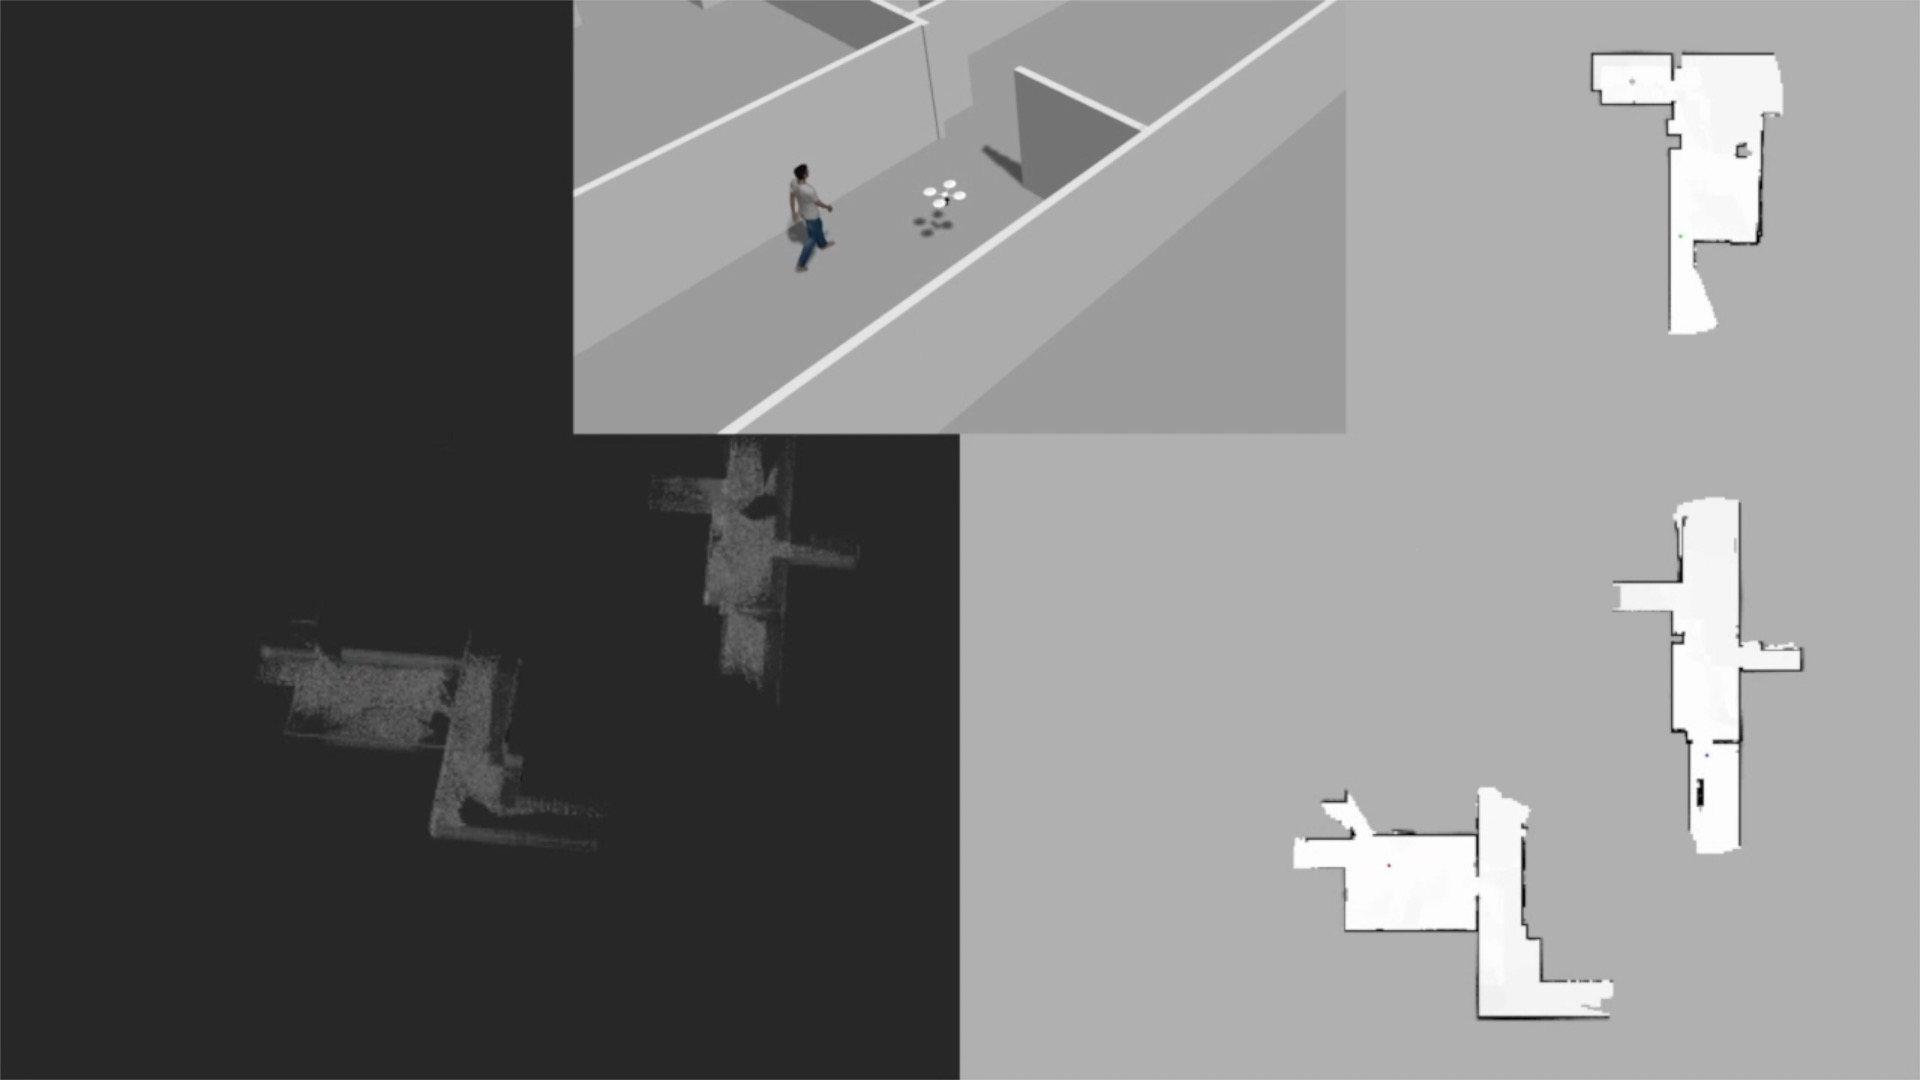
\includegraphics[trim={22cm 25cm 20cm 0cm}, clip, width=\textwidth]{evade_15sec.jpg}
        		\caption{$15$ sec}
    	\end{subfigure}
	\hspace*{0.02\textwidth}
    	\begin{subfigure}[t]{0.3\columnwidth}
           	\centering
          	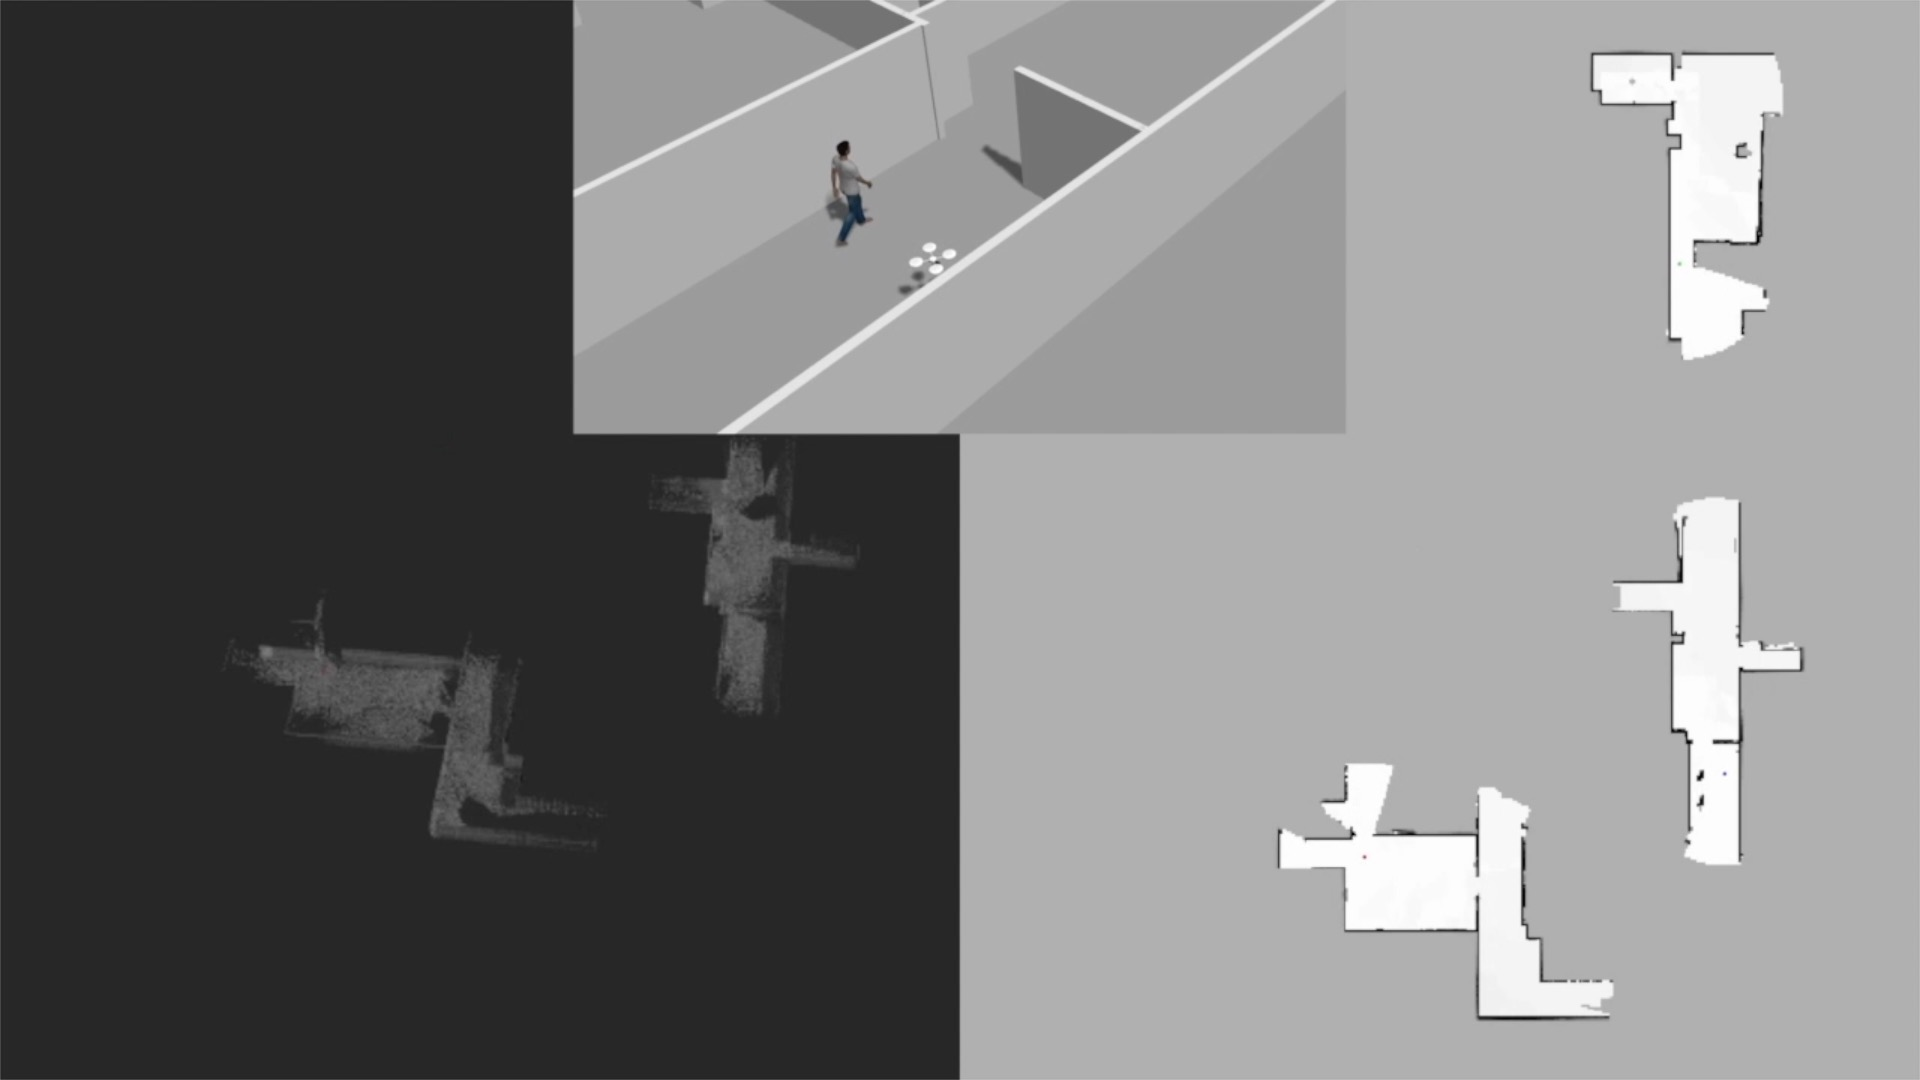
\includegraphics[trim={22cm 25cm 20cm 0cm}, clip, width=\textwidth]{evade_16sec.jpg}
        		\caption{$16$ sec}
    	\end{subfigure}
	\hspace*{0.02\textwidth}
    	\begin{subfigure}[t]{0.3\columnwidth}
           	\centering
          	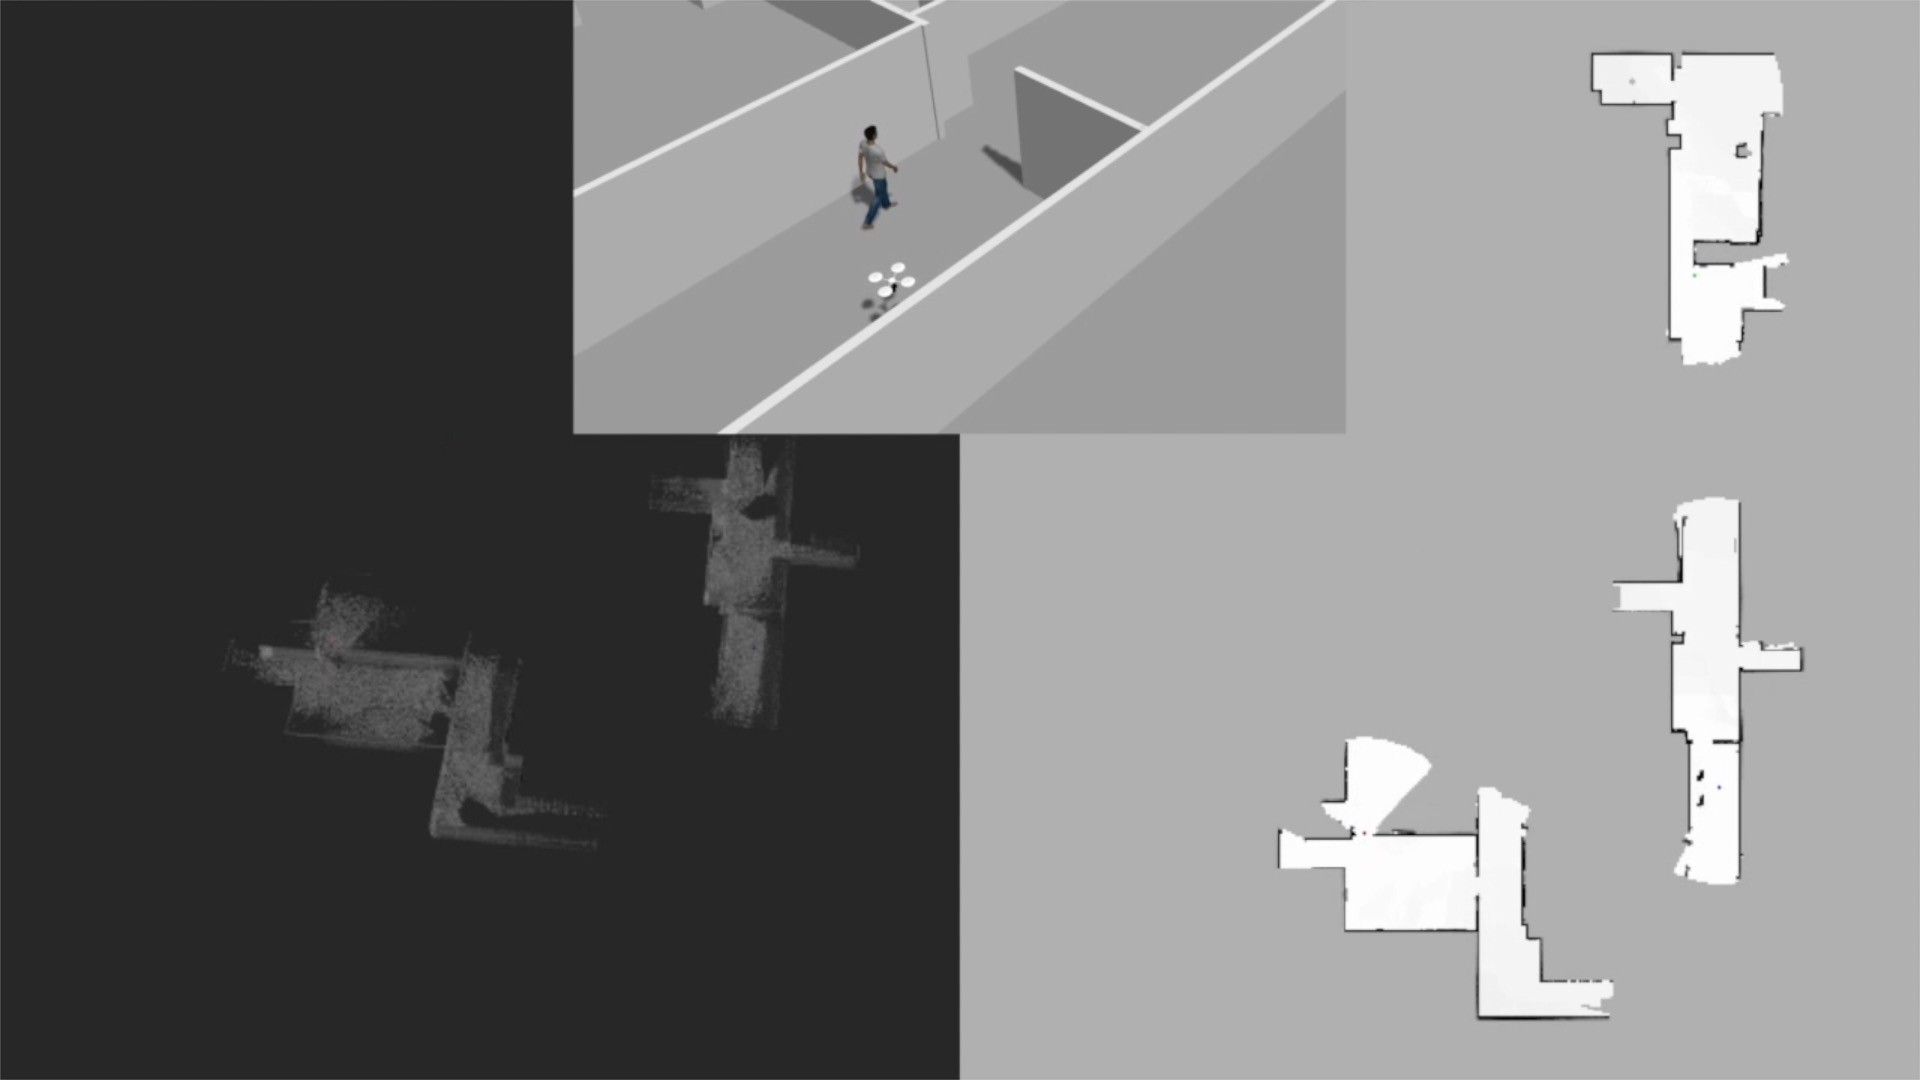
\includegraphics[trim={22cm 25cm 20cm 0cm}, clip, width=\textwidth]{evade_17sec.jpg}
        		\caption{$17$ sec}
    	\end{subfigure}
	\caption{A cooperating robot must evade a non-cooperative human. The receding horizon framework allows a quickly-updating map to modify the exploration commands to avoid collisions with a dynamic obstacle.}
	\label{fig:EvadeHuman}
\end{figure}

The results also demonstrate an interesting tradeoff between exploring new terrain and patrolling previously-visited spaces. When the degradation rate $\lambda$ is increased, grid cells are degrading faster, incentivizing the exploration strategy to revisit spaces faster. This behavior is beneficial for frequent patrol, but certain areas, particularly those difficult to reach, are not visited as quickly or as frequently. Should an area receive extra attention, a greater value of $\lambda$ may be applied to this region.


\section{Conclusions}
\label{sec:Conclusions}

This paper introduces a near-optimal bidding-based solution to multi-vehicle exploration and patrol to map a 3D space. This approach integrates recent developments in obtaining occupancy grid probabilities and entropies into several auctions to assign tasks to robots. The bidding process relies on expected map information gains and travel distances, and modifies bids between auctions to promote robotic cooperation. Information gains are modified by updating a temporary expected map, and an additional term prevents collisions among robots. Grid cells are continuously degraded using a continuous-time Markov process, which incentivizes the autonomous exploration-based patrol scheme to revisit regions after time passes. Furthermore, a receding horizon constantly updates the bidding process and improves collision avoidance within a dynamic environment. The efficacy of the approach is shown with a numerical simulation patrolling a large floor plan with a walking human, with several computational enhancements for scalability of the algorithms.

The research presented in this paper may be enhanced in several ways. First, this research assumes fixed map limits. In practice, a robot may not be given knowledge of the environment size. A mapping and exploration algorithm that is capable of expanding as it explores could increase the number of applications for such robots. Additionally, localization can be challenging in uncertain environments. Therefore, localization can be included in the exploration policy. The uncertainty of the robot pose estimate could further improve the accuracy of the probabilistic map, expected entropy calculations, and collision-avoidance.



%\section*{Appendix}\label{append}
%
%
%\subsection*{Proof of Proposition 1}
%
%Continuous Markov process

\bibliography{../../BibSources}
\bibliographystyle{IEEEtran}

\vspace*{0.1\textwidth}

\noindent{\bf Evan Kaufman} is a robotics engineer at Robotic Research LLC. He received his B.S. degree in Mechanical Engineering from Bucknell University in 2012, and his Ph.D. in Aerospace Engineering at The George Washington University in 2018. His research focusses are in robotic mapping and exploration with range-based sensors, estimation, data association, and flight controls. He has worked on several research projects through the U.S. Air Force Research Laboratory and Naval Research Laboratory.

\vspace*{0.1\textwidth}

\noindent{\bf Kuya Takami} is a scientific software developer at Enthought and was a postdoctoral research fellow at the Department of Mechanical and Aerospace Engineering at the George Washington University. He received his doctoral degree in Mechanical Engineering at Virginia Polytechnic Institute and State University in 2015 specializing in robot perception. His main interests include mobile robot perception and autonomous systems.


\vspace*{0.1\textwidth}

\noindent{\bf Zhuming Ai} is a Computer Engineer in the Information Technology Division at the U.S. Naval Research Laboratory (NRL). Before he joined NRL, he served as the Director of the Virtual Reality in Medicine Lab at the University of Illinois at Chicago. He is interested in virtual reality, augmented reality, computer graphics, image processing, and robotics.

\vspace*{0.1\textwidth}

\noindent{\bf Taeyoung Lee} is an associate professor of the Department of Mechanical and Aerospace Engineering at The George Washington University. He received his doctoral degree in Aerospace Engineering and his master?s degree in Mathematics at the University of Michigan in 2008. His research interests include geometric mechanics and control with applications to complex aerospace systems.










\end{document}

